\documentclass[12pt, cleqn, a4paper]{article}

\usepackage[utf8]{inputenc}
\usepackage[T2A]{fontenc}
\usepackage{amssymb,amsmath,mathrsfs,amsthm}
\usepackage[english, russian]{babel}
\usepackage{caption}
\usepackage[pdftex]{graphicx}
\usepackage{epsfig}
\usepackage{subfig}
\usepackage{indentfirst}
\usepackage{hyperref}
\usepackage{xcolor}
\usepackage{svg}
\usepackage{calc}
\usepackage{float}

\textheight=24cm
\textwidth=16cm
\oddsidemargin=5mm
\evensidemargin=-5mm
\marginparwidth=36pt
\topmargin=-2cm
\footnotesep=3ex
\setlength{\parskip}{6pt}
\flushbottom
\raggedbottom
\tolerance 3000
\clubpenalty=10000
\widowpenalty=10000
\renewcommand{\baselinestretch}{1.1}
\renewcommand{\baselinestretch}{1.5}
\linespread{1.5}
\definecolor{linkcolor}{HTML}{000000}
\definecolor{citecolor}{HTML}{000000}
\definecolor{urlcolor}{HTML}{0000FF}
\hypersetup{pdfstartview=FitH, linkcolor=linkcolor, citecolor=citecolor, urlcolor=urlcolor, colorlinks=true}
\bibliographystyle{unsrt}

\graphicspath{{images/}}

\newcommand{\anonsection}[1]{\section*{#1}\addcontentsline{toc}{section}{#1}}
\newcommand{\bfv}[1]{\mathbf{#1}}
\newcommand{\dd}[1]{\dot{#1}}
\newcommand{\dvp}[3]{#1\,\times\,[\,#2\,\times\,#3\,]}
\newcommand{\dv}[1]{\nabla v(#1)}
\newcommand{\ddv}[1]{\mathrm{D}[v](#1)}
\newcommand{\dr}{\delta \bfv{r}}
\newcommand{\dn}{\delta \bfv{n}}
\newcommand{\om}[1]{\mathrm{o}(#1)}
\newcommand{\dprod}[2]{\langle #1, #2 \rangle}
\newcommand{\T}[1]{#1^\mathrm{T}}
\newcommand{\matr}[1]{\mathrm{#1}}
\newcommand{\hr}{\hat{\bfv{r}}}

\begin{document}

\begin{titlepage}
\begin{center}
    Московский государственный университет имени М. В. Ломоносова

    \bigskip
    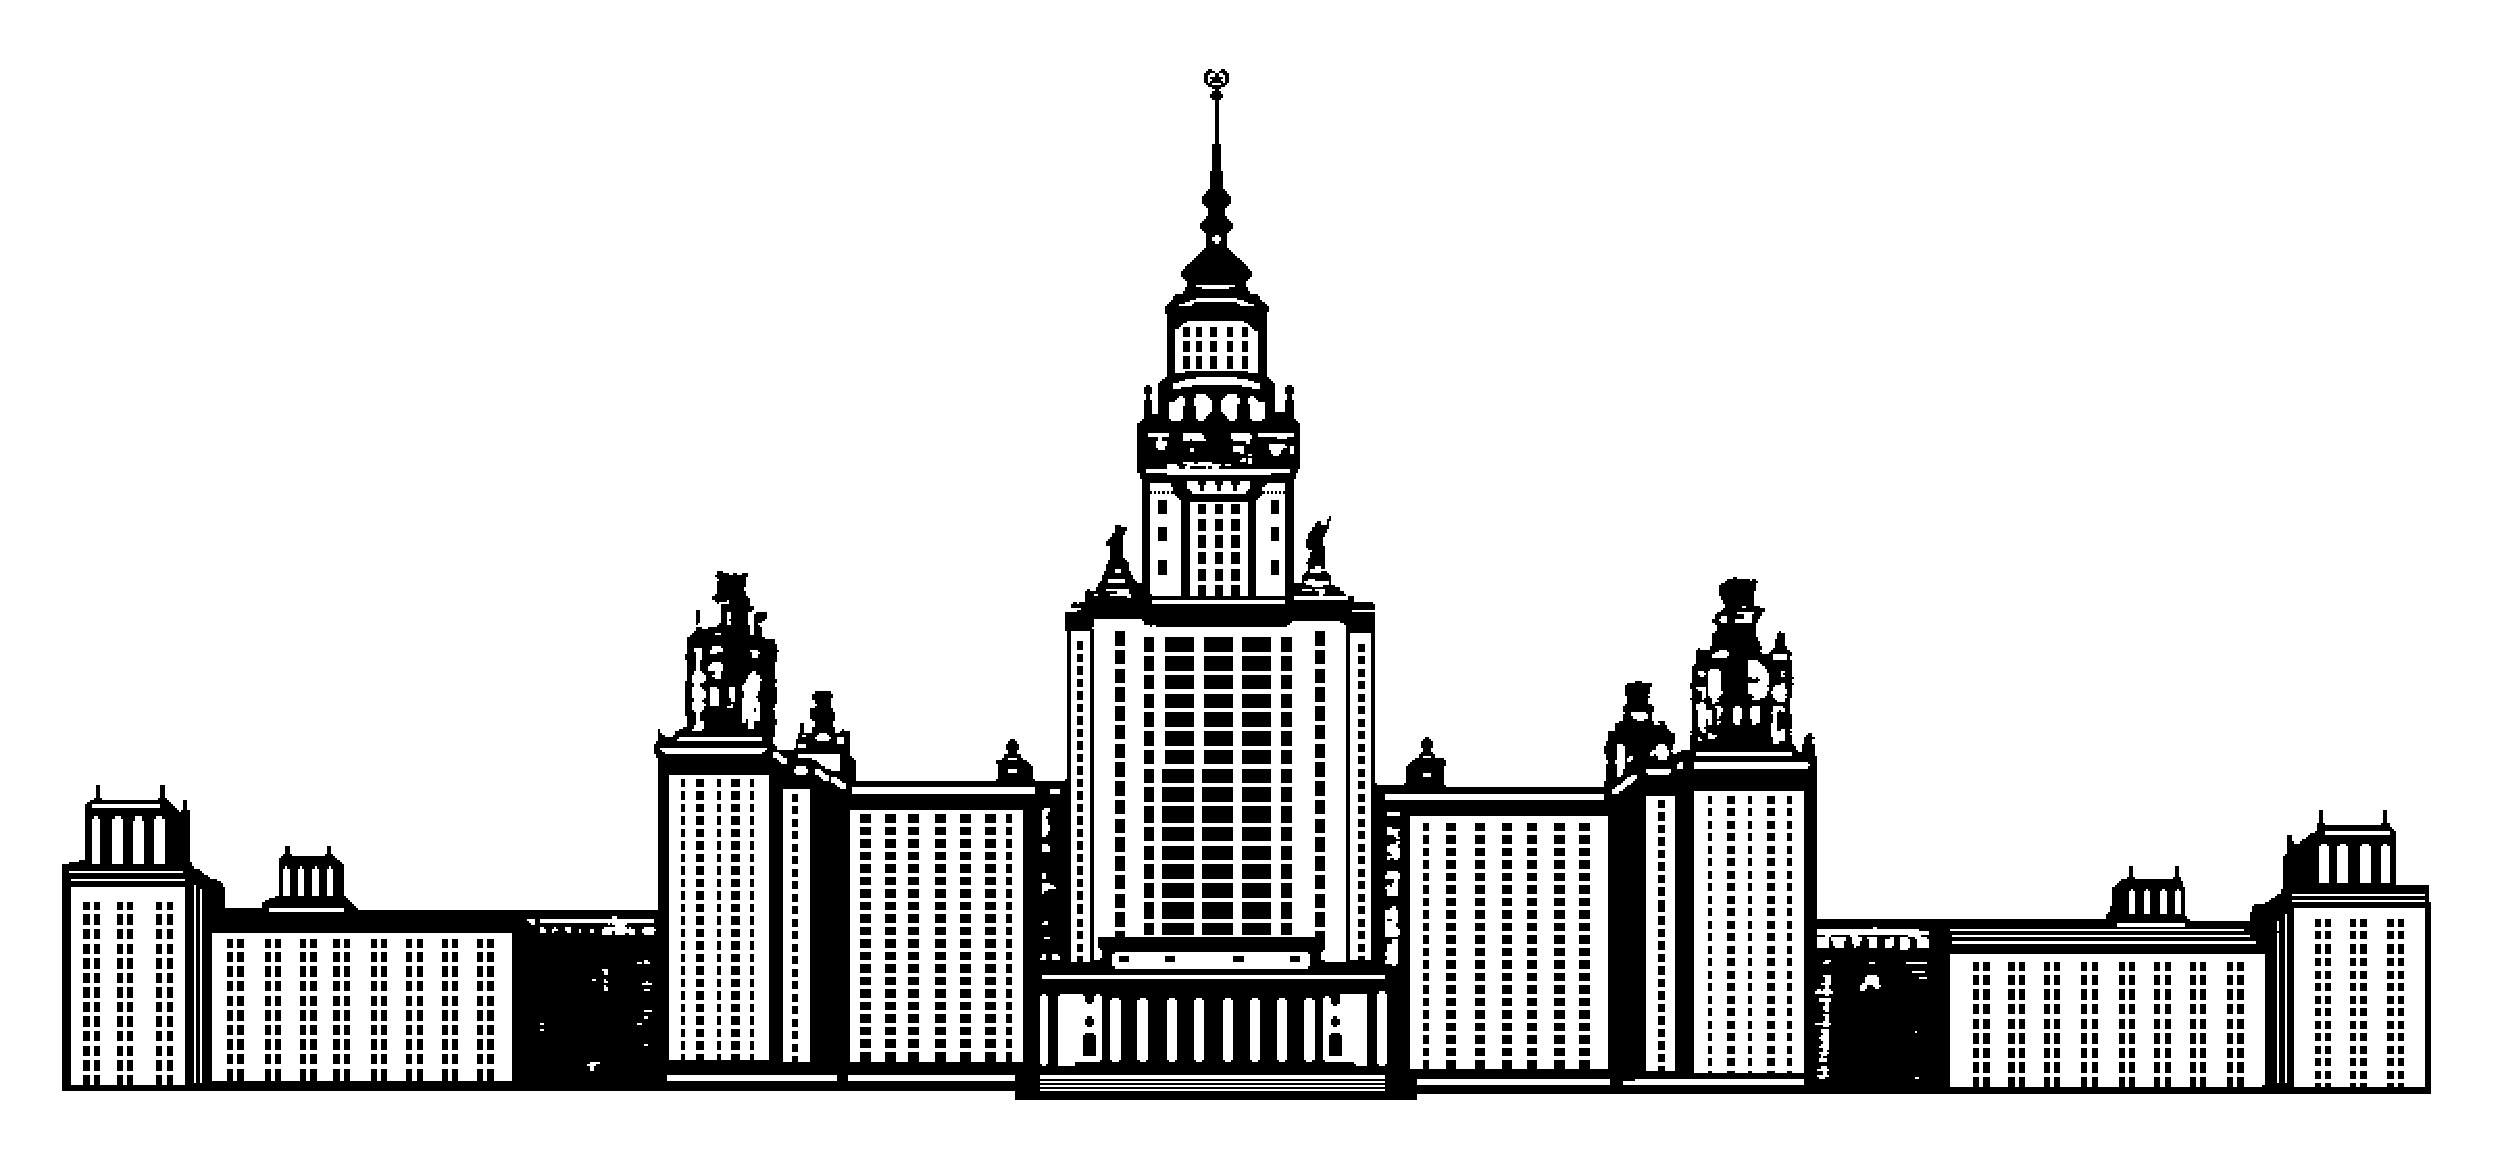
\includegraphics[width=50mm]{msu.eps}

    \bigskip
    Факультет вычислительной математики и кибернетики
    
    Кафедра математической физики\\[10mm]

    \textsf{\large\bfseries
        ПРЕДДИПЛОМНАЯ ПРАКТИЧЕСКАЯ РАБОТА\\[10mm]
        <<Реализация градиентных методов решения обратной задачи распространения луча в неоднородной среде>>
    }\\[30mm]

    \begin{flushright}
        \parbox{0.35\textwidth}{
            Выполнил:\\
            студент 401 группы\\
            \emph{Зубков~Егор~Александрович}\\[10mm]
            Научный руководитель:\\
            д.ф-м.н., профессор\\
            \emph{Баев~Андрей~Владимирович}\\[2mm]
            к.ф-м.н., с.н.с.\\
            \emph{Иванов~Антон~Валерьевич}
        }
    \end{flushright}

    

    \vspace{\fill}
    Москва, 2021
\end{center}
\end{titlepage}

%--------------------------------------------------------------------------------------------------------
\newpage
\renewcommand{\contentsname}{Содержание}
\tableofcontents
%--------------------------------------------------------------------------------------------------------
\newpage
\begin{abstract}

В данной работе исследуются методы решения одной из ключевых задач подзадач моделирования распространения сейсмических волн в неоднородной среде --- поддержание линейных параметров сетки, задающей волновой фронт. В ходе работы предложен алгоритм добавления дополнительных вершин посредством выбора особых начальных направлений лучей, а также представлена структура поддержки связей для нерегулярной сетки. В результате был реализован алгоритм,и его работоспособность проверена на модельных параметрах.

\end{abstract}

%--------------------------------------------------------------------------------------------------------
\newpage
\anonsection{Введение}
Среди всех современных средств изучения структуры земной коры, наиболее точным и часто используемым является сейсморазведка. Для сбора сейсмоданных, в рамках данного метода, вначале производятся специальные сейсморазведочные работы. На земной поверхности располагают геофоны, которые регистрируют рассеянные и отраженные волны от глубинных поверхностей. Источником этих волн являются взрывы в неглубоких шахтах, расположенных в заданных местах. Типичный размер исследуемой области $10^3$ - $10^4$ $\text{м}^2$~\cite{kirchhoff}.

Наиболее совершенным методом реконструкции изображения по полученным в результате сейсморазведки данным является «3-мерная глубинная миграция до
суммирования»~\cite{kirchhoff, multiarrival, thomsen1986weak}.

\begin{figure}[H]
    \centering
    \begin{tabular}{cc}
    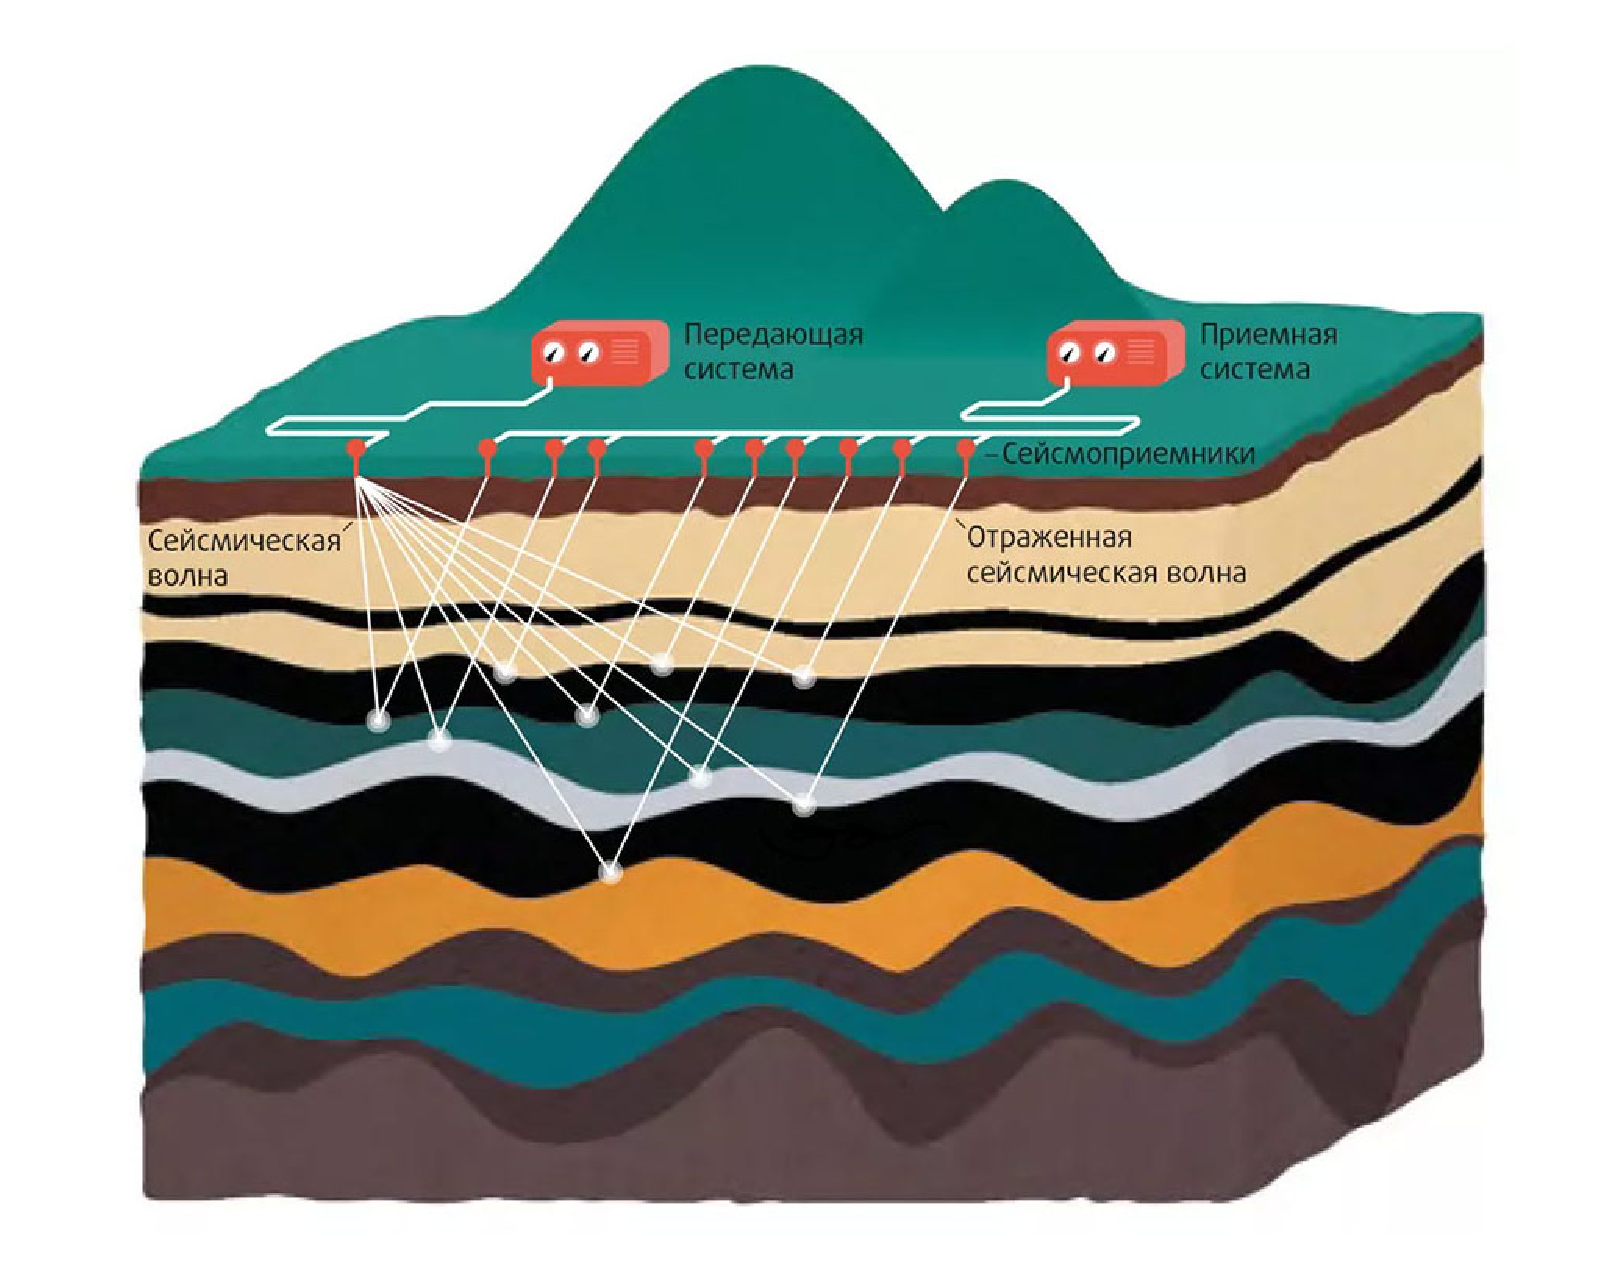
\includegraphics[width=0.5\linewidth]{model_seismic_survey.eps}
    &
    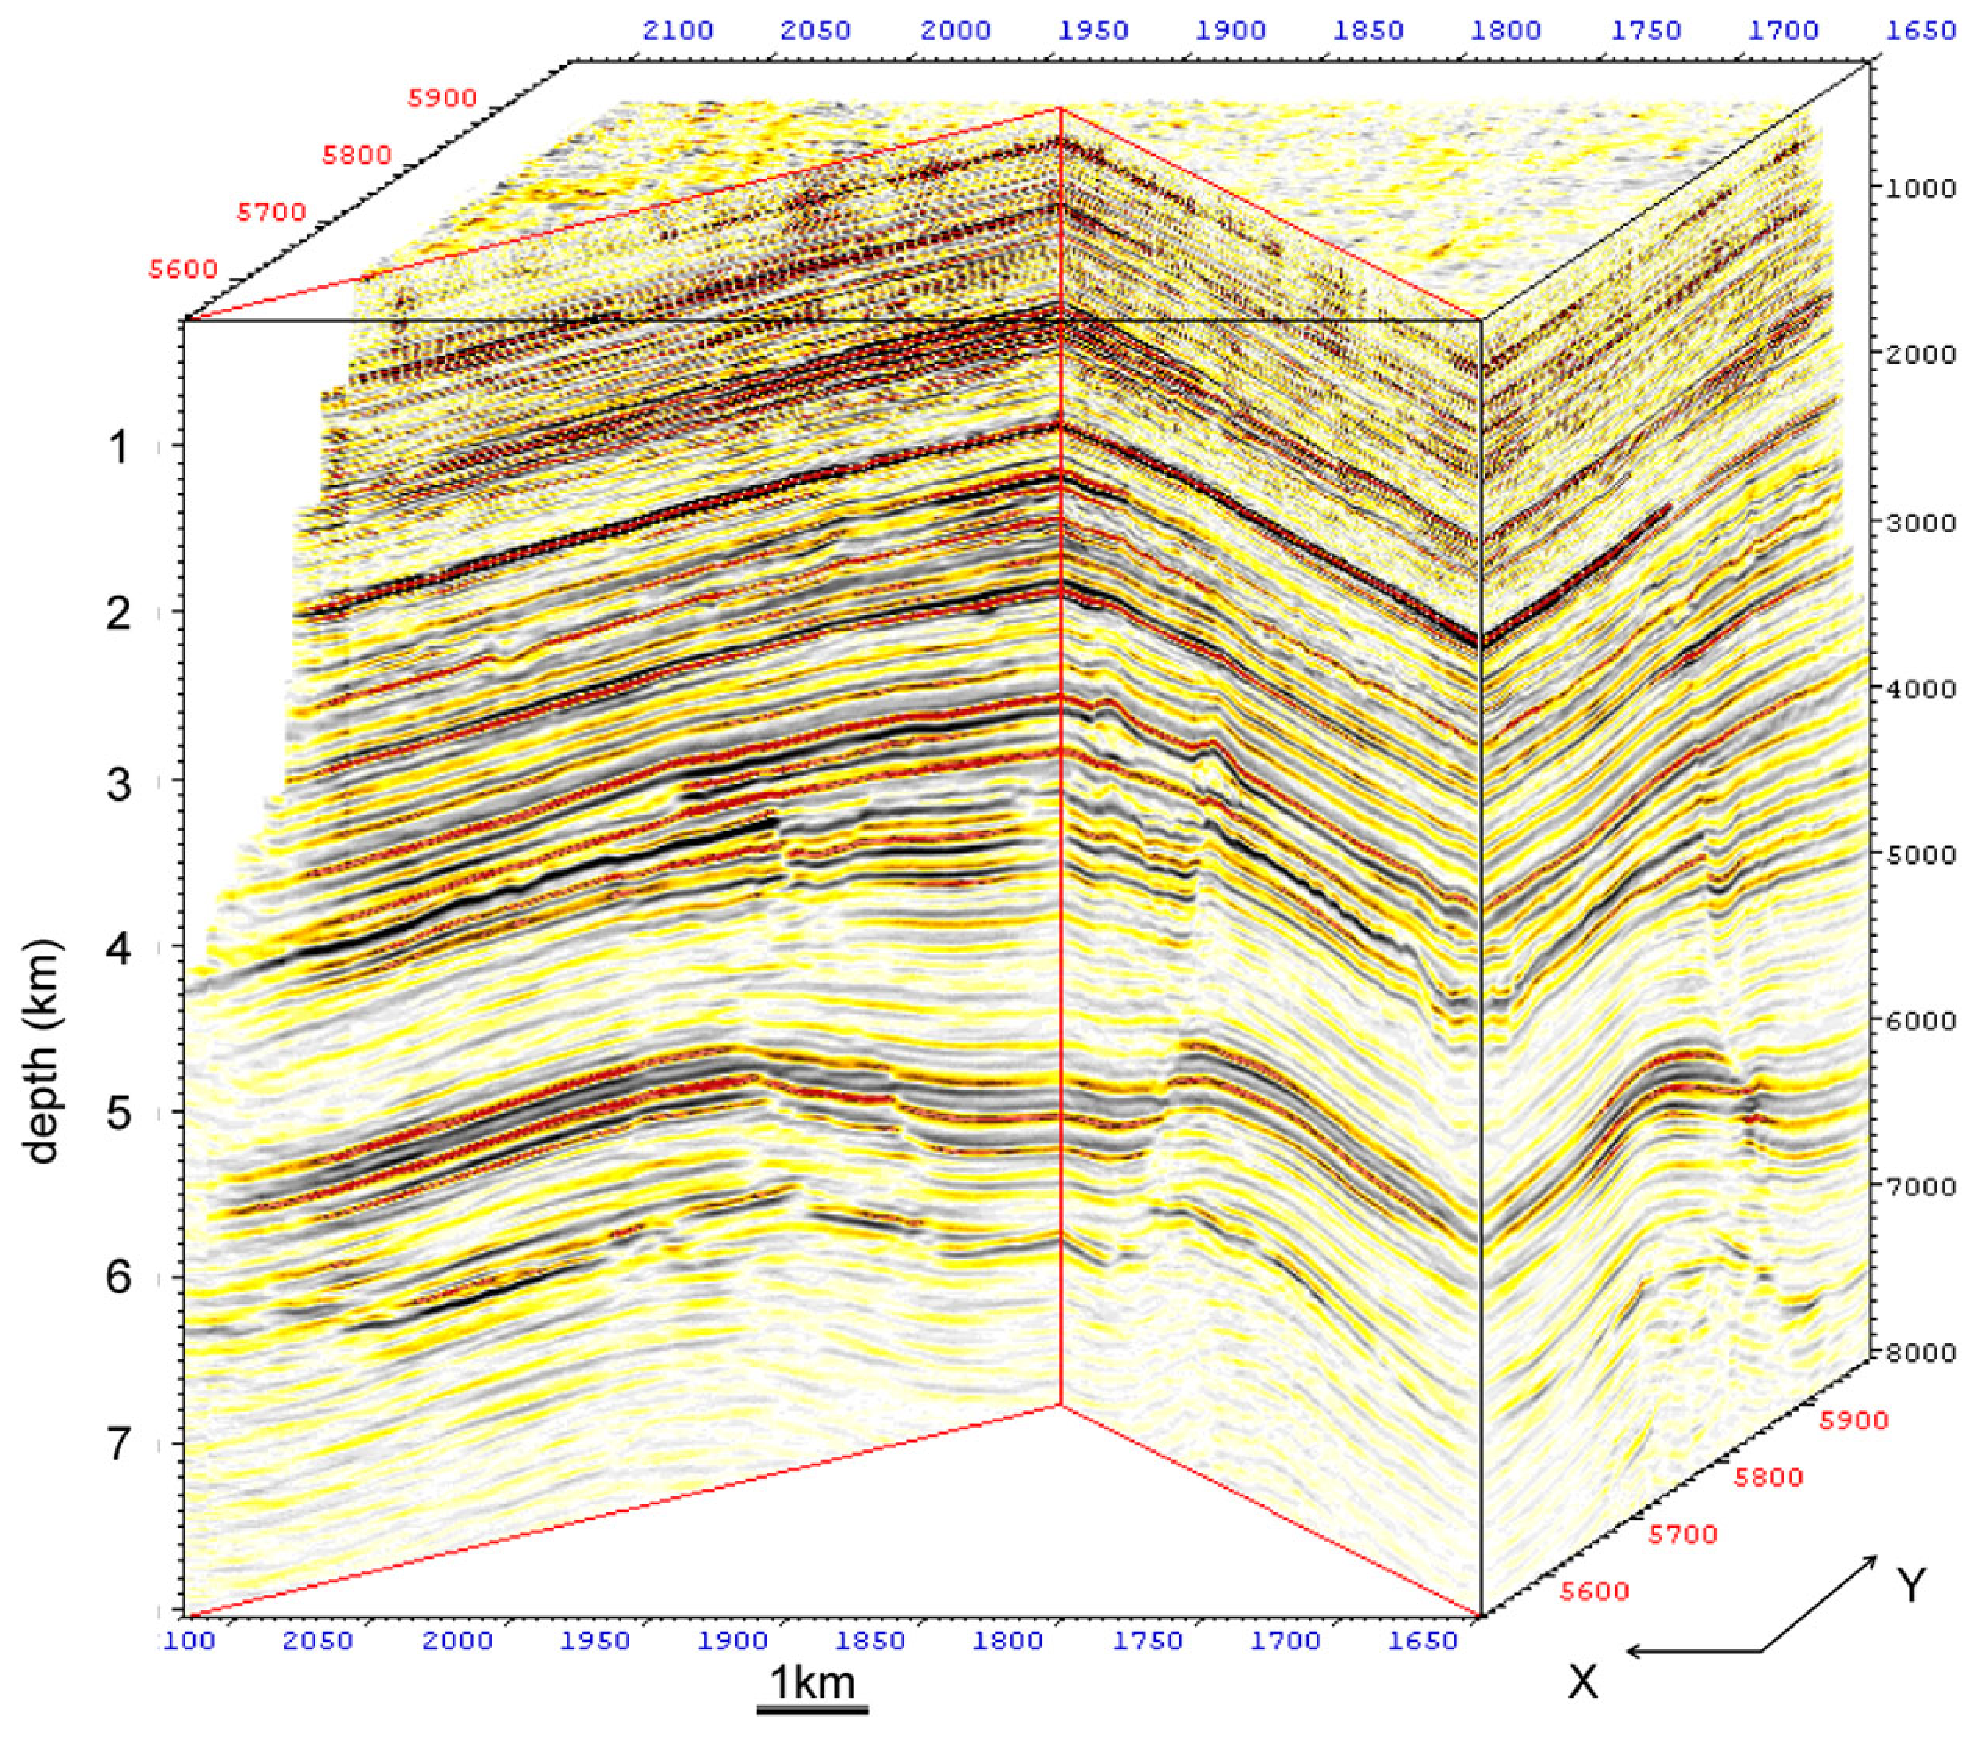
\includegraphics[width=0.4\linewidth]{seismic_image.eps}
    \end{tabular}
    \caption{Модель проведения сейсморазведки и результат работы алгоритма.}
\end{figure}

Важной подзадачей в ходе реализации данного алгоритма является поддержание заданных размеров ребра сетки, на которой выполняются вычисления. Сама сетка представляет собой триангуляцию волнового фронта, в качестве вершин в которой содержатся концы лучей. 

Рассмотрим два возможных способа решения данной задачи. В первой возможно простое перестроение сетки путем перекидывания ребра внутри двух треугольников. Это возможно, когда длина второй диагонали соответствует заданным ограничениям. Второй подход заключается в добавлении новой вершины в сетку, и преобразованию двух треугольников в четыре с меньшими ребрами.

\begin{figure}[H]
    \centering
    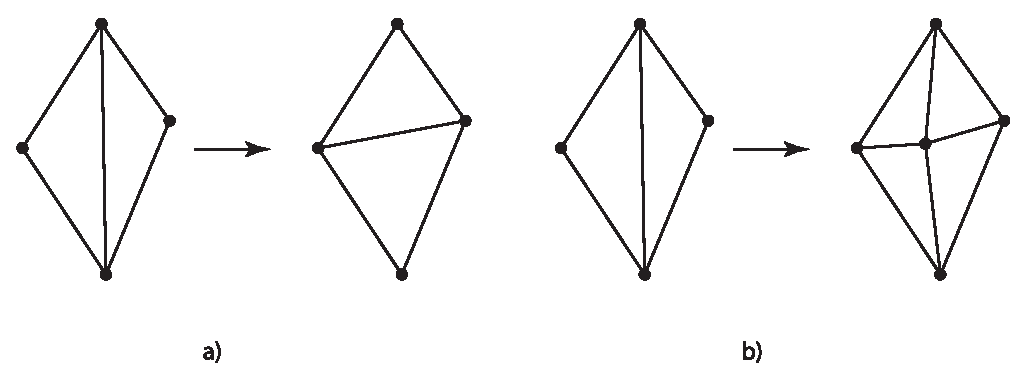
\includegraphics[width=0.8\linewidth]{transform_edge.eps}
    \caption{Способы преобразования сетки.}
\end{figure}

Реализация второго способа является существенно более затратной по сравнению с первой, однако существуют ситуации, когда он является единственно возможным.

В работе предлагается базовая и градиентная реализация второго метода перестроения сетки.

%--------------------------------------------------------------------------------------------------------
\newpage
\section{Постановка прямой и обратной задачи}
Как было отмечено ранее, для аппроксимации волнового фронта используется нерегулярная сетка, представляющая собой триангуляцию волнового фронта. Ключевой проблемой ее применимости является увеличение длины ребер за счет расхода лучей с течением времени. 

Введем вначале несколько связанных с сеткой определений, а также запишем математическую постановку прямой и обратной задачи.

\subsection{Определения и обозначения}
Рассмотрим более подробно и формализуем ее три основных примитива --- луч, лучевую трубку и ребро лучевой трубки.

$\bullet\;$ \textbf{Луч} --- совокупность двух характеристик: $\bfv{r}$ и $\bfv{n}$, заданных в каждый момент времени $t$ и определяющих, соответственно, текущее положение и направление его конца.

$\bullet\;$ \textbf{Лучевая трубка} --- абстракция, являющаяся объединением трех ближайших лучей. Является ячейкой нашей сетки.

\begin{figure}[h!]
    \centering
    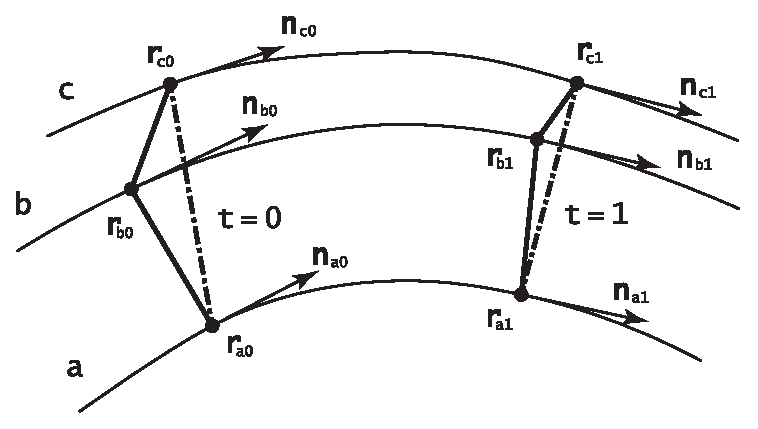
\includegraphics[width=0.6\linewidth]{tube.eps}
    \caption{Лучевая трубка. Приведены два состояния в момент  $t = 0$ и $t = 1$.}
\end{figure}

$\bullet\;$ \textbf{Ребро лучевой трубки} (далее просто ребро) --- объединение пар лучей из лучевой трубки. Его длину мы определим как евклидову норму разности радиус-векторов концов.

\subsection{Постановка прямой задачи}
В качестве прямой задачи рассматривается моделирование движения отдельного луча в пространстве. Оно задается следующей системой:
\begin{equation} \label{eq:01}
\begin{cases}
\dd{\bfv{r}} = v(\bfv{r})\,\bfv{n}, &\tau > 0\\
\dd{\bfv{n}} = \dvp{\bfv{n}}{\bfv{n}}{\dv{\bfv{r}}}, &\tau > 0\\
\bfv{r}|_{\tau=0} = \bfv{r}_0 \quad \bfv{n}|_{\tau=0} = \bfv{n}_0
\end{cases}
\end{equation}
Распределение скоростей $v(\bfv{r})$ и его градиент $\dv{\bfv{r}}$ определяются средой и считаются известными.

\subsection{Постановка обратной задачи}
Далее будем рассматривать лишь ребра нашей сетки, длина которых больше заданного ограничения. Обратной задачей будет являться восстановление начального направления луча $\bfv{n}_0$ при заданных начальном $\bfv{r}_0$ и конечном в момент времени $\tau = t$ $\bfv{r}_{end}$ положениях. В качестве $\bfv{r}_{end}$ выберем середину рассматриваемого ребра --- $\hr$.

Данную задачу можно формализовать как задачу оптимизации следующего функционала:
\begin{equation} \label{eq:02}
J(\bfv{n}_0) = \big\|\matr{T}\,\big(\bfv{r}\,(\bfv{n}_0, \bfv{r}_0, t) \ - \ \hr \big)\big\|_2 \rightarrow \min_{\bfv{n}_0\,\in\,N}
\end{equation}

Матрица $\matr{T}$ является матрицей перехода в барицентрические координаты. В качестве опорных точек используются вершины соседних по рассматриваемому ребру лучевых трубок. 

%--------------------------------------------------------------------------------------------------------
\newpage
\section{Нахождение градиентов бихарактеристик луча}
Рассмотрим исходную систему бихарактеристик луча в переменных $\bfv{r}$ и $\bfv{n}$:
\begin{equation} \label{eq:11}
\begin{cases}
\dd{\bfv{r}} = v(\bfv{r})\,\bfv{n}, &\tau > 0\\
\dd{\bfv{n}} = \dvp{\bfv{n}}{\bfv{n}}{\dv{\bfv{r}}}, &\tau > 0\\
\bfv{r}|_{\tau=0} = \bfv{r}_0 \quad \bfv{n}|_{\tau=0} = \bfv{n}_0
\end{cases}
\end{equation}

\noindentИз физических соображений $\bfv{n}$ --- единичная нормаль к волновому фронту $\Rightarrow \ \|\bfv{n}\|~=~1$.

\noindentВоспользуемся тождеством Лагранжа для двойного векторного произведения \\ $\dvp{\bfv{n}}{\bfv{n}}{\dv{\bfv{r}}}$:
\begin{equation} \label{eq:12}
    \dvp{\bfv{n}}{\bfv{n}}{\dv{\bfv{r}}} = \bfv{n}\,\dprod{\bfv{n}}{\dv{\bfv{r}}} - \dv{\bfv{r}}\,\dprod{\bfv{n}}{\bfv{n}} = \bfv{n}\,\dprod{\bfv{n}}{\dv{\bfv{r}}} - \dv{\bfv{r}}
\end{equation}\

\noindentПодставляя \eqref{eq:12} в \eqref{eq:11}, получим:
\begin{equation} \label{eq:13}
\begin{cases}
\dd{\bfv{r}} = v(\bfv{r})\,\bfv{n}\\
\dd{\bfv{n}} =  \bfv{n}\,\dprod{\bfv{n}}{\dv{\bfv{r}}} - \dv{\bfv{r}}\\
\end{cases}
\end{equation}\vspace{1mm}

Рассмотрим малое возмущение для $\bfv{r}$ и $\bfv{n}$:
\begin{align*}
\bfv{r_1} &= \bfv{r} + \dr   &   \bfv{n_1} &= \bfv{n} + \dn
\end{align*}

\noindentБудем считать, что в линейном приближении система \eqref{eq:13} верна для переменных $\bfv{r_1}$~и~$\bfv{n_1}$, то есть: 
\begin{equation} \label{eq:14}
\begin{cases}
\dd{\bfv{r_1}} = v(\bfv{r_1})\,\bfv{n_1} + \om{\|\dr\| + \|\dn\|}\\
\dd{\bfv{n_1}} = \bfv{n_1}\,\dprod{\bfv{n_1}}{\dv{\bfv{r_1}}} - \dv{\bfv{r_1}} + \om{\|\dr\| + \|\dn\|}\\
\end{cases}
\end{equation}

\noindentРазложим в ряд Тейлора функции $v(\bfv{r})$ и $\dv{\bfv{r}}$:
\begin{gather*} 
v(\bfv{r_1}) = v(\bfv{r}) + \dprod{\dv{\bfv{r}}}{\dr} + \om{\|\dr\|}\\ 
\dv{\bfv{r_1}} = \dv{\bfv{r}} + \ddv{\bfv{r}}\,\dr + \om{\|\dr\|}
\end{gather*}

\noindentПодставим полученные разложения в систему \eqref{eq:14}, воспользовавшись формулой Лагранжа для двойного векторного произведения: 
\begin{equation} \label{eq:15}
\begin{cases}
\dd{\bfv{r}} + \dd{\dr} = v(\bfv{r})\,\bfv{n} + \dprod{\dv{\bfv{r}}}{\dr}\,\bfv{n} + v(\bfv{r})\,\dn + \om{\|\dr\| + \|\dn\|}\\
\dd{\bfv{n}} + \dd{\dn} = \bfv{n}\,\dprod{\bfv{n}}{\dv{\bfv{r}}} - \dv{\bfv{r}} + \dn\,\dprod{\bfv{n}}{\dv{\bfv{r}}} + \bfv{n}\,\dprod{\dn}{\dv{\bfv{r}}} + \\ 
\qquad + \bfv{n}\,\dprod{\bfv{n}}{\ddv{\bfv{r}}\dr} - \ddv{\bfv{r}}\dr + \om{\|\dr\| + \|\dn\|}\\
\end{cases}
\end{equation}

\noindentИспользуя равенства системы \eqref{eq:11}, перепишем \eqref{eq:15} в следующем виде:
\begin{equation*}
\begin{cases}
\dd{\dr} = \dprod{\dv{\bfv{r}}}{\dr}\,\bfv{n} + v(\bfv{r})\,\dn + \om{\|\dr\| + \|\dn\|}\\
\dd{\dn} = \dn\,\dprod{\bfv{n}}{\dv{\bfv{r}}} + \bfv{n}\,\dprod{\dn}{\dv{\bfv{r}}} + \bfv{n}\,\dprod{\bfv{n}}{\ddv{\bfv{r}}\dr} - \ddv{\bfv{r}}\dr + \om{\|\dr\| + \|\dn\|}
\end{cases}
\end{equation*}

\noindentЧто эквивалентно следующей записи:
\begin{equation} \label{eq:16}
\begin{cases}
\dd{\dr} = \bfv{n}\T{\dv{\bfv{r}}}\,\dr + v(\bfv{r})\,\dn + \om{\|\dr\| + \|\dn\|}\\
\dd{\dn} = \dprod{\bfv{n}}{\dv{\bfv{r}}}\,\dn + \bfv{n}\T{\dv{\bfv{r}}}\,\dn + \bfv{n}\T{\bfv{n}}\,\ddv{\bfv{r}}\,\dr - \ddv{\bfv{r}}\,\dr + \om{\|\dr\| + \|\dn\|}
\end{cases}
\end{equation}\vspace{1mm}

В силу сферичности фронта положим $\dr = \matr{P}(\tau)\,\dn_0$ и $\dn = \matr{Q}(\tau)\,\dn_0$ и оставим только линейные $\delta$-члены. Сгруппируем по $\dn_0$, и в результате система \eqref{eq:16} примет вид:
\begin{equation} \label{eq:17}
\begin{cases}
\dd{\matr{P}} = \bfv{n}\T{\dv{\bfv{r}}}\,\matr{P} + v(\bfv{r})\,\matr{Q}\\
\dd{\matr{Q}} = (\bfv{n}\T{\bfv{n}} - \matr{I})\,\ddv{\bfv{r}}\,\matr{P} + (\bfv{n}\T{\dv{\bfv{r}}} + \dprod{\bfv{n}}{\dv{\bfv{r}}}\,\matr{I})\,\matr{Q}\\
\matr{P}|_{\tau=0} = \matr{\O} \quad \matr{Q}|_{\tau=0} = \matr{I}
\end{cases}
\end{equation}

\noindentВ матричном виде \eqref{eq:17}:
\begin{equation} \label{eq:18}
\begin{cases}
\dd{\matr{P}} = \matr{M}_{11}(\tau)\,\matr{P} + \matr{M}_{12}(\tau)\,\matr{Q}\\
\dd{\matr{Q}} = \matr{M}_{21}(\tau)\,\matr{P} + \matr{M}_{22}(\tau)\,\matr{Q} 
\end{cases}, \ \text{где}
\end{equation}

\begin{equation}
\begin{aligned} \label{eq:19}
\matr{M}_{11}(\tau) = \bfv{n}(\tau)\T{\dv{\bfv{r}(\tau)}} \mspace{105mu}  &\matr{M}_{12}(\tau) = v(\bfv{r}(\tau))\,\matr{I}\\
\matr{M}_{21}(\tau) = (\bfv{n}(\tau)\T{\bfv{n}(\tau)} - \matr{I})\,\ddv{\bfv{r}(\tau)} \quad &\matr{M}_{22}(\tau) = \bfv{n}(\tau)\T{\dv{\bfv{r}(\tau)}} + \dprod{\bfv{n}(\tau)}{\dv{\bfv{r}(\tau)}}\,\matr{I}
\end{aligned}
\end{equation}

Решения системы \eqref{eq:18} -- матрицы $\matr{P}$ и $\matr{Q}$, соответственно, задают первые производные бихарактеристик $\bfv{r}$ и $\bfv{n}$ по начальному направлению $\bfv{n_0}$.

%--------------------------------------------------------------------------------------------------------
\newpage
\section{Алгоритм решение прямой задачи}
Для решения системы \eqref{eq:01} будем использовать явный метод Рунге-Кутты 4~порядка~\cite{wanner1996solving}.
Введем следующее обозначения:
\begin{equation} \label{eq:21}
\begin{gathered}
\bfv{y} = \T{(\bfv{r},\ \bfv{n})}, \\
\bfv{f}(\tau,\,\bfv{y}) \equiv \bfv{f}(\bfv{y}) = \T{\Bigl(v(\bfv{r})\,\bfv{n},\ \bfv{n}\,\dprod{\bfv{n}}{\dv{\bfv{r}}} - \dv{\bfv{r}}\Bigr)} 
\end{gathered}
\end{equation}\vspace{1mm}

\noindentЗаменяя переменные согласно \eqref{eq:21}, исходная система \eqref{eq:01} принимает вид:
\begin{equation}\label{eq:22}
\begin{cases}
\dd{\bfv{y}} = \bfv{f}(\bfv{y}) \\
\bfv{y}|_{\tau=0} = \bfv{y}_0\\
\end{cases}
\end{equation}\vspace{1mm}

\noindentСогласно методу, приближенное решение системы \eqref{eq:22} задается следующими формулами:
\begin{equation}
\begin{gathered}
\bfv{y}_{n+1} = \bfv{y}_n + \frac{h}{6}\,\Bigl(\,\bfv{k}_1 + 2\,\bfv{k}_2 + 2\,\bfv{k}_3 + \bfv{k}_4\,\Bigr)\text{, где} \\
\bfv{k}_1 = \bfv{f}(\bfv{y}_n), \quad \bfv{k}_2 = \bfv{f}\Bigl(\bfv{y}_n + \dfrac{h}{2}\,\bfv{k}_1 \Bigr), \\
\bfv{k}_3 = \bfv{f}\Bigl(\bfv{y}_n + \frac{h}{2}\,\bfv{k}_2\Bigr), \quad \bfv{k}_4 = \bfv{f}\Bigl(\bfv{y}_n + h\,\bfv{k}_3\Bigr)
\end{gathered}
\end{equation}

В качестве вспомогательных средств активно применялась библиотека aiwlib \cite{aiwlib}.

%--------------------------------------------------------------------------------------------------------
\newpage
\section{Алгоритм решения обратной задачи}
\subsection{Алгоритм построения сетки}
Первым этапом решения поставленной задачи является создание неструктурированной сетки. Основным свойством подобной сетки является возможность динамического добавления новых вершин, получаемых в ходе решения обратной задачи, а также перестроения ее с учетом разбиения лучевых трубок.

Рассмотрим сетку как неориентированный граф, вершинами в котором будут являться лучевые трубки. Для получения вершин будем применять обход в ширину~\cite{cormen2009introduction, tarjan1983data}.

\begin{figure}[h!]
\begin{minipage}[h!]{0.39\linewidth}
\centering
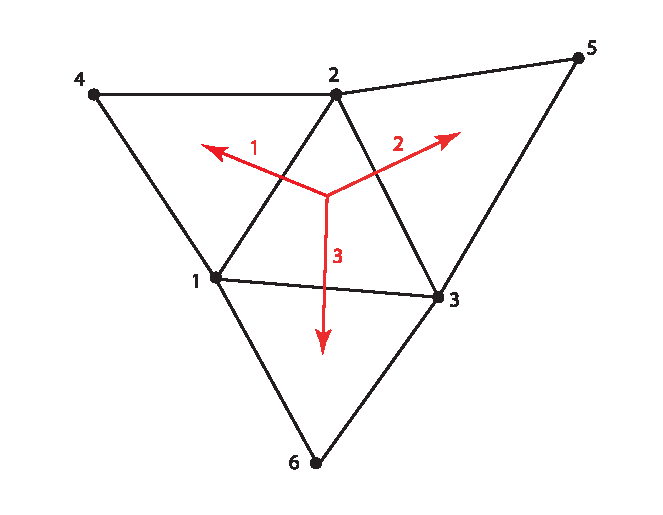
\includegraphics[width=1.2\linewidth]{grid_bfs.eps}
\caption*{a)}
\end{minipage}
\hfill
\begin{minipage}[h!]{0.59\linewidth}
\centering
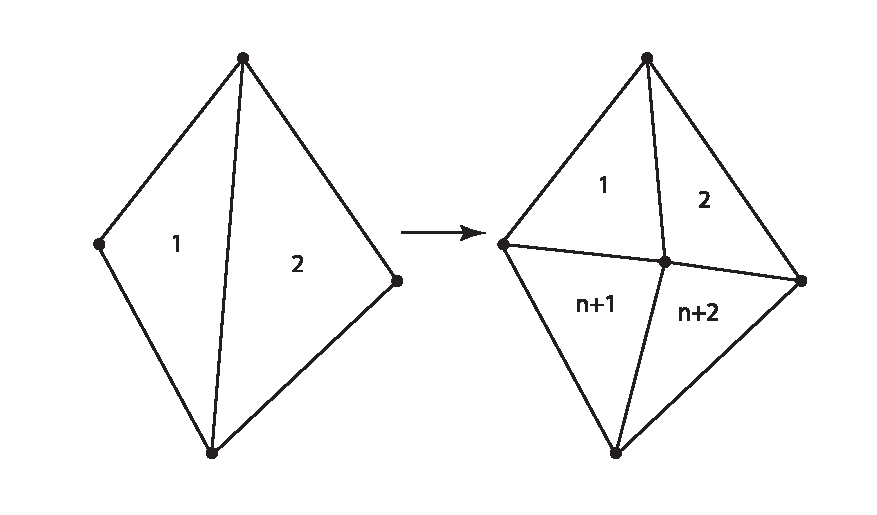
\includegraphics[width=1.1\linewidth]{grid_rebinding.eps}
\caption*{b)}
\end{minipage}
\caption{\quad a) Обход сетки для получения лучей.}
\caption*{b) Создание новых трубок при добавлении нового луча.}
\label{fig:grid}
\end{figure}

\noindentНа рис. \ref{fig:grid} a) представлен такой обход для выбранной вершины графа. Стрелками указаны переходы между вершинами, порядок лучей соответствует представленным номерам. На рис. \ref{fig:grid} b) показано добавление вершин в граф после вычисления нового луча. При этом создаются две новые трубки, а также меняется одна из вершин в старых.

\subsection{Оптимизация методом простого перебора}
В качестве первого метода решения обратной задачи рассмотрим простой перебор. Это наиболее простой алгоритм, который можно использовать в качестве базового решения для теста работы алгоритма построения сетки и сравнения эффективности работы последующих методов.

Как было отмечено ранее, исходная обратная задачу сводится к оптимизационной задаче с ограничениями. Будем предполагать, что искомое начальное направление луча $\bfv{n}_0$ лежит во множестве $N$. Оно определяется как пирамида, образованная четырьмя лучами из двух смежных по разбиваемому ребру лучевых трубок (тремя в случае, если разбиваемое ребро -- граничное).
\begin{figure}[h!]
    \centering
    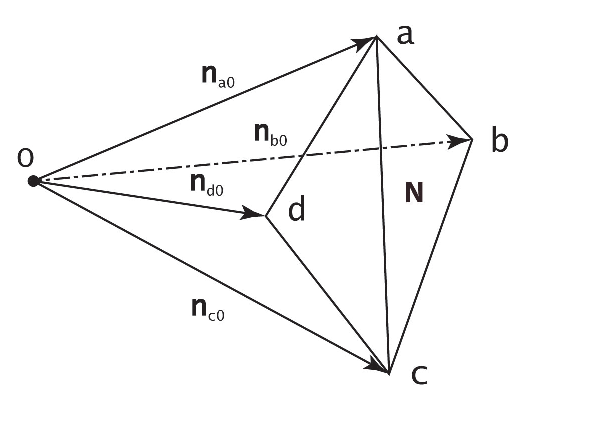
\includegraphics[width=0.5\linewidth]{set.eps}
    \caption{Множество $N$ для ребра $ac$ с двумя смежными лучевыми трубками $abc$ и $acd$.}
\end{figure}

Начальное направление луча $\bfv{n}_0$ будем получать как среднее между ближайшими лучами. 

Введем понятие сетки пирамиды. Она состоит из уже ранее рассмотренных начальных направлений, находящихся внутри пирамиды. 

Каждую такую фазу дробления текущего состояния назовем рангом. Первый ранг такого разбиения состоит из середин ребер четырехугольника и большей его диагонали. Второй ранг содержит середины ребер, образованных при добавлении к изначальной фигуре в качестве вершин лучей из первого ранга. Далее эта операция повторяется аналогично для следующих порядков.

\begin{figure}[h!]
    \centering
    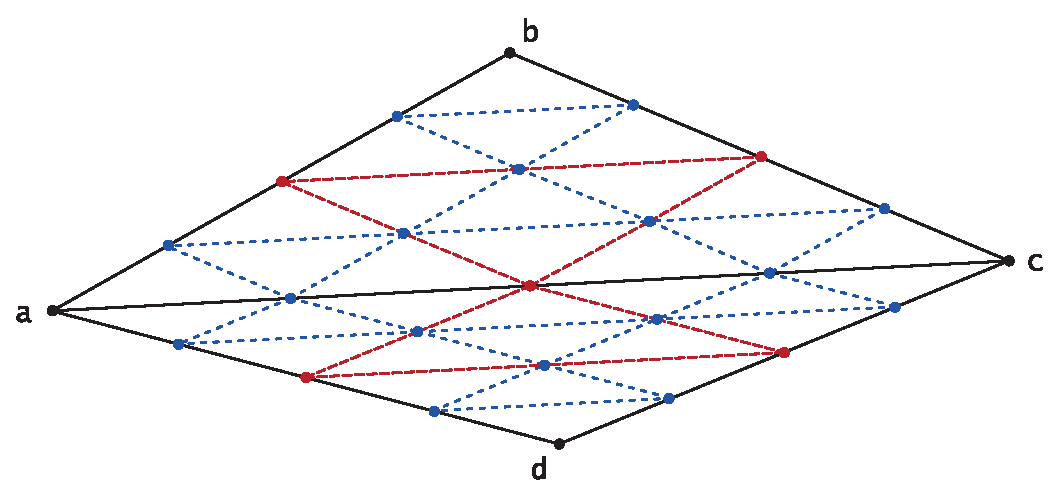
\includegraphics[width=0.9\linewidth]{rank.eps}
    \caption{Лучи для первых трех рангов сетки пирамиды для ребра $ac$. Черные -- 1 ранга, красные -- 2 ранга, синие -- 3 ранга.}
\end{figure}

Ограничим количество разбиений 7 рангами для большей производительности. Формально, это может привести к тому, что луч, удовлетворяющий ограничениям не будет найден. Однако, исходя из величины лучевых трубок и условий на величину функционала, такие случаи редки, что в дальнейшем подтверждается экспериментами.  

Алгоритм решения состоит из следующих этапов:
\begin{enumerate} 
    \item Выполняем один шаг трассировки всех лучей сетки (шаг решения прямой задачи).
    \item Просматриваем каждое из ребер и выбираем такие, длина которых превышает заданное ограничение.
    \item Для каждого выбранного ребра выполняем поиск подходящего для его разбиения луча (в соответствии с описанным ранее алгоритмом).
    \item Выполняем разбиение, создаем новые трубки, заменяем лучи в них и пересвязываем для поддержания структуры сетки.
\end{enumerate}

\subsection{Оптимизация методом градиентного спуска}
Первый этап для всех градиентных методов заключается в выражении градиента исходного функционала через известные величины и градиенты по параметру $\bfv{n}_0$. Для удобства также вместо самого функционала будем рассматривать его квадрат. 
\begin{equation} \label{eq:31}
\nabla \hat{J}(\bfv{n}_0) = \nabla_{\bfv{n}_0}\big\|\matr{T}\,\big(\bfv{r}\,(\bfv{n}_0, \bfv{r}_0, t) \ - \ \hr \big)\big\|^2_2 =\frac{d\hat{J}}{d\bfv{r}}\,\frac{d\bfv{r}}{d\bfv{n}_0} = 2\,\T{\matr{P}}\T{\matr{T}}\matr{T}\,(\bfv{r} - \hr)
\end{equation}

Матрица $\matr{P}$ определяет производную $\bfv{r}$ по параметру $\bfv{n}_0$ и находится из системы~\eqref{eq:18}.

Опишем теперь сам алгоритм градиентного спуска~\cite{vasiliev2002methods}. Он представляет собой итерационный алгоритм, который задается следующей формулой:
\begin{equation} \label{eq:32}
\bfv{n}_{k+1} = \bfv{n}_k - \lambda_k \nabla \hat{J}(\bfv{n}_k)
\end{equation}

На размер шага $\lambda_k$ существует теоретическое ограничение, в предположении липшицевости градиента:
\begin{equation*}
\| \nabla \hat{J}(\bfv{x}) -  \nabla \hat{J}(\bfv{y})\| < L\|x - y\|, \quad \forall \, x,\,y
\end{equation*}
\noindentТогда при $\lambda_k < \dfrac{2}{L}$ гарантируется убывание $\hat{J}(\bfv{n}_k)$.

На практике, подбор шага производится эмпирически.

\subsection{Оптимизация методом градиентного спуска с импульсом}
Модифицируем алгоритм градиентного спуска. Его итерационная формула имеет вид:
\begin{equation} \label{eq:32}
\bfv{n}_{k+1} = \bfv{n}_k - \lambda_k \nabla \hat{J}(\bfv{n}_k) - \beta_k (\bfv{n}_k - \bfv{n}_{k-1})
\end{equation}

Коэффициент $\beta_k = \gamma_k\dfrac{\dprod{\nabla \hat{J}(\bfv{n}_k)}{\nabla \hat{J}(\bfv{n}_k)}}{\dprod{\nabla \hat{J}(\bfv{n}_{k-1})}{\nabla \hat{J}(\bfv{n}_{k-1})}}$ --- Метод Флетчера---Ривса~\cite{dennis1996numerical, nesterov1984methods}.

%--------------------------------------------------------------------------------------------------------
\newpage
\section{Экспериментальная проверка алгоритмов}
Проверка работоспособности алгоритма состоит из нескольких этапов: решение прямой задачи, вычисление градиентов $\matr{P}$ и $\matr{Q}$ из системы \eqref{eq:18}, решение обратной задачи рассмотренными методами.

\subsection{Модельные параметры задачи}
Для описания параметров задачи необходимо задать начальное положение источника волн и поле скоростей, характеризующее пропускаемость среды.

\noindentВ качестве модельного распределения скоростей используется следующая функция:
\begin{equation*}
v(\bfv{r}) = v_0 - \Delta v\,\exp\Biggl(\,\dfrac{-(\bfv{r} - \bfv{r}_0)^2}{2\sigma^2}\,\Biggr)
\end{equation*}

\noindentСоответствующие константы имеют следующие значения:
\begin{equation*}
\bfv{r}_0 = (\,0,\,0,\,3000\,)^T, \ v_0 = 2000\,\dfrac{\text{м}}{\text{с}}, \ \Delta v = 1000\,\dfrac{\text{м}}{\text{с}}, \ \sigma = 750\,\text{м}
\end{equation*}

\begin{figure}[h!]
\noindent
\centering
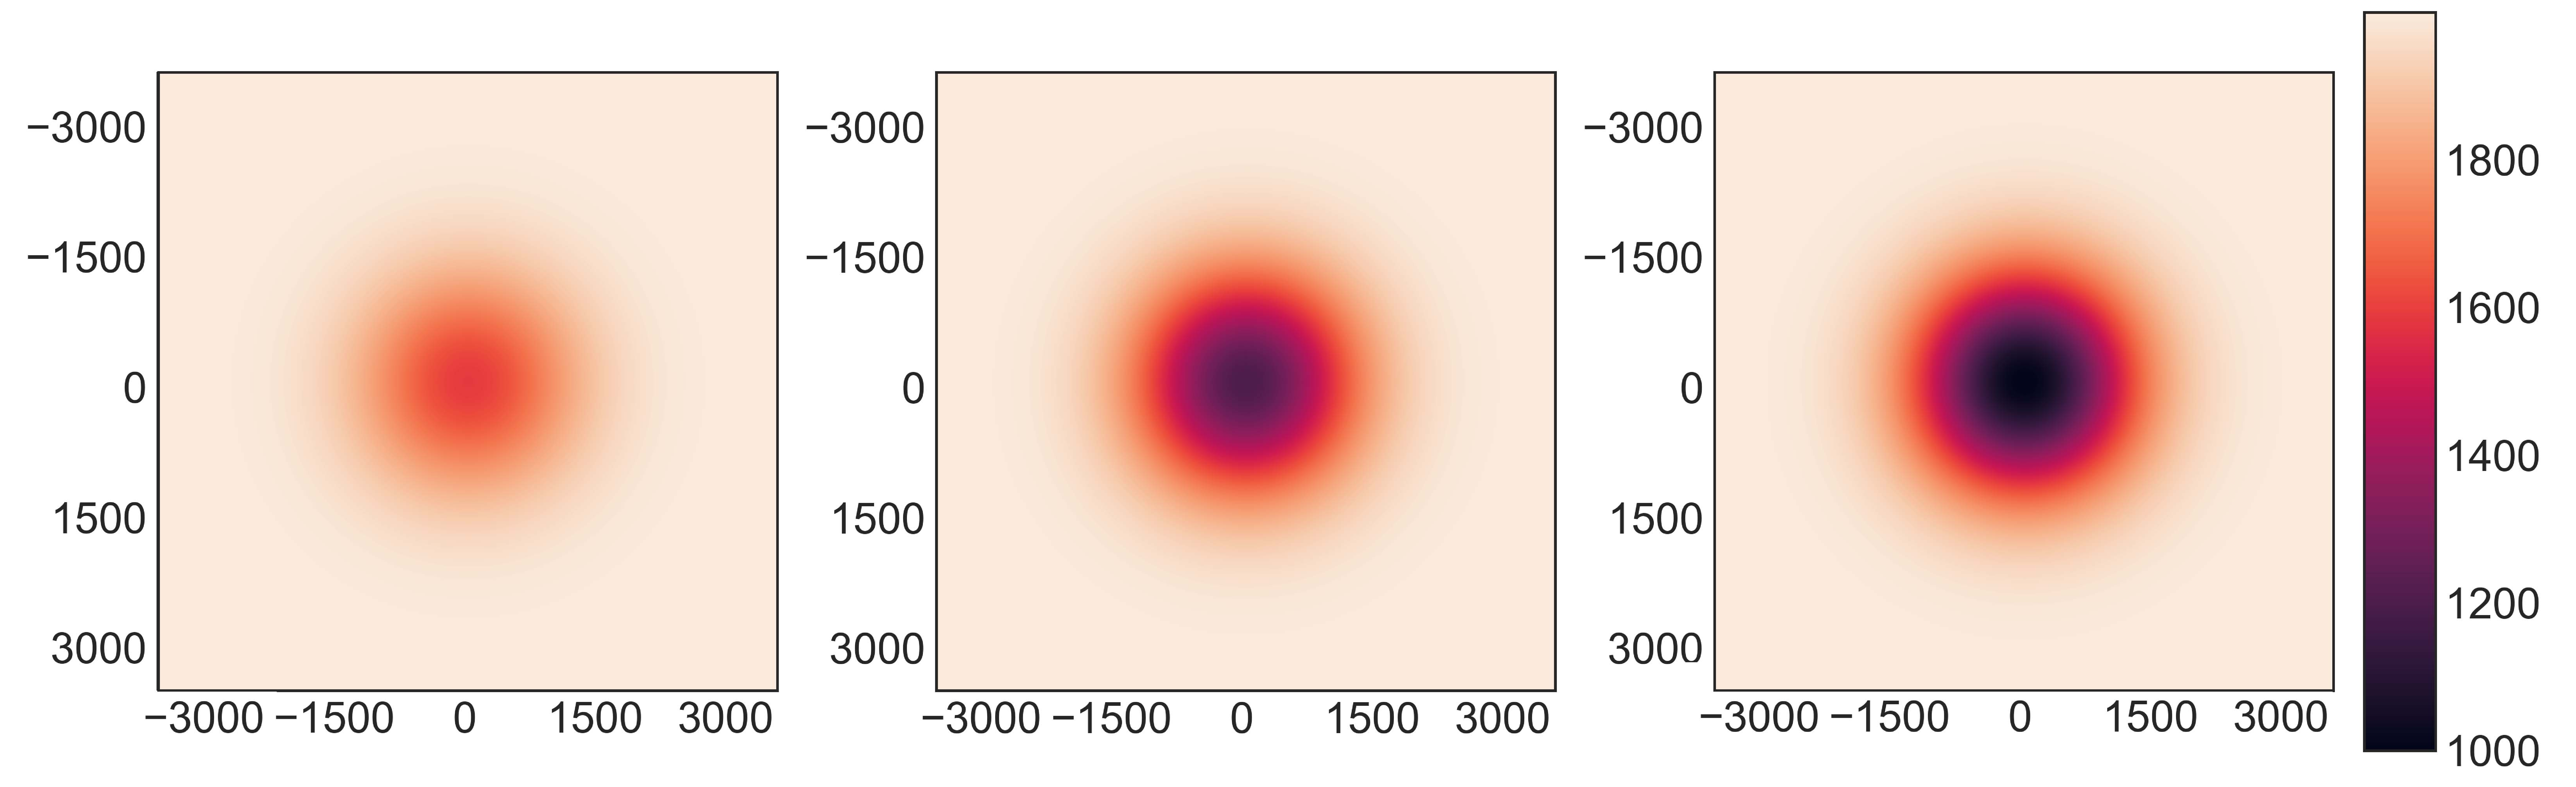
\includegraphics[width=1.0\linewidth]{field_speed.eps}
\caption{Двумерные проекции распределения скоростей при $z = 1500,\ 2000, \ 3000$.}
\end{figure}

\noindentДлину ребра сетки ограничим 500\,м.

\subsection{Тестирование вычисления градиентов характеристик луча}
Тестирование вычисления градиентов будем проводить по следующей схеме. 

\noindentРассмотрим несколько начальных направлений $\bfv{n}_0$, концы которых равномерно распределены на поверхности сферы единичного радиуса. Посчитаем для моментов времени $\tau$ значения $\bfv{r}(\tau)$ и $\matr{P}(\tau)$, соответствующих им. Далее зададим для каждого $\bfv{n}_0$ малые ортогональные отклонения $\dn_0$. В качестве показателя точности будем использовать значение нормы отклонения линейного приближения: 
\begin{equation} \label{eq:41}
\|\bfv{r}_1(\tau) - (\bfv{r}(\tau) + \matr{P}(\tau)\,\dn_0)\|^2, \ \text{где $\bfv{r}_1$ -- решение системы \eqref{eq:14}, $\bfv{r}$ -- системы \eqref{eq:11}}
\end{equation}

\noindentДля тестирование градиентов введем два вспомогательных поля скоростей:

\subsubsection{Константное поле скоростей}
Рассмотрим следующее константное поле скоростей:
\begin{equation*}
v(\bfv{r}) = a \ \forall \ r \in R
\end{equation*}

\noindentЛегко видеть, что:
\begin{align*}
\dv{\bfv{r}} &= \T{(0,\,0,\,0)}  &   \ddv{\bfv{r}} &= \matr{\O}
\end{align*}

\noindentСледовательно, матрицы $\matr{M}_{11}$, $\matr{M}_{12}$, $\matr{M}_{21}$ и $\matr{M}_{22}$ \eqref{eq:19} записываются как:
\begin{align*} 
&\matr{M}_{11}(\tau) = \matr{\O}&\matr{M}_{12}(\tau) = a\,\matr{I}\\
&\matr{M}_{21}(\tau) = \matr{\O}&\matr{M}_{22}(\tau) = \matr{\O}
\end{align*}

\noindentВ результате система \eqref{eq:18} примет следующий вид:
\begin{equation} \label{eq:41}
\begin{cases}
\dd{\matr{P}} = a\,\matr{Q}\\
\dd{\matr{Q}} = \matr{\O}\\
\matr{P}|_{\tau=0} = \matr{\O}; \ \matr{Q}|_{\tau=0} = \matr{I}
\end{cases}
\end{equation}

\noindentЕе решение легко находится:
\begin{equation} \label{eq:42}
\begin{cases}
\matr{P}(\tau) = a\tau\,\matr{I}\\
\matr{Q}(\tau) = \matr{I}
\end{cases}
\end{equation}

\noindentПоложим для теста $a = 500$\,м/с, и рассмотрим численные значения норм отклонений \eqref{eq:41} для различных моментов времени.

Пусть также нормы векторов $\dn_0$ логравномерно распределены в диапазоне от $10^{-1}$ до $10^{-2}$\,м.

\begin{figure}[H] 
\centering
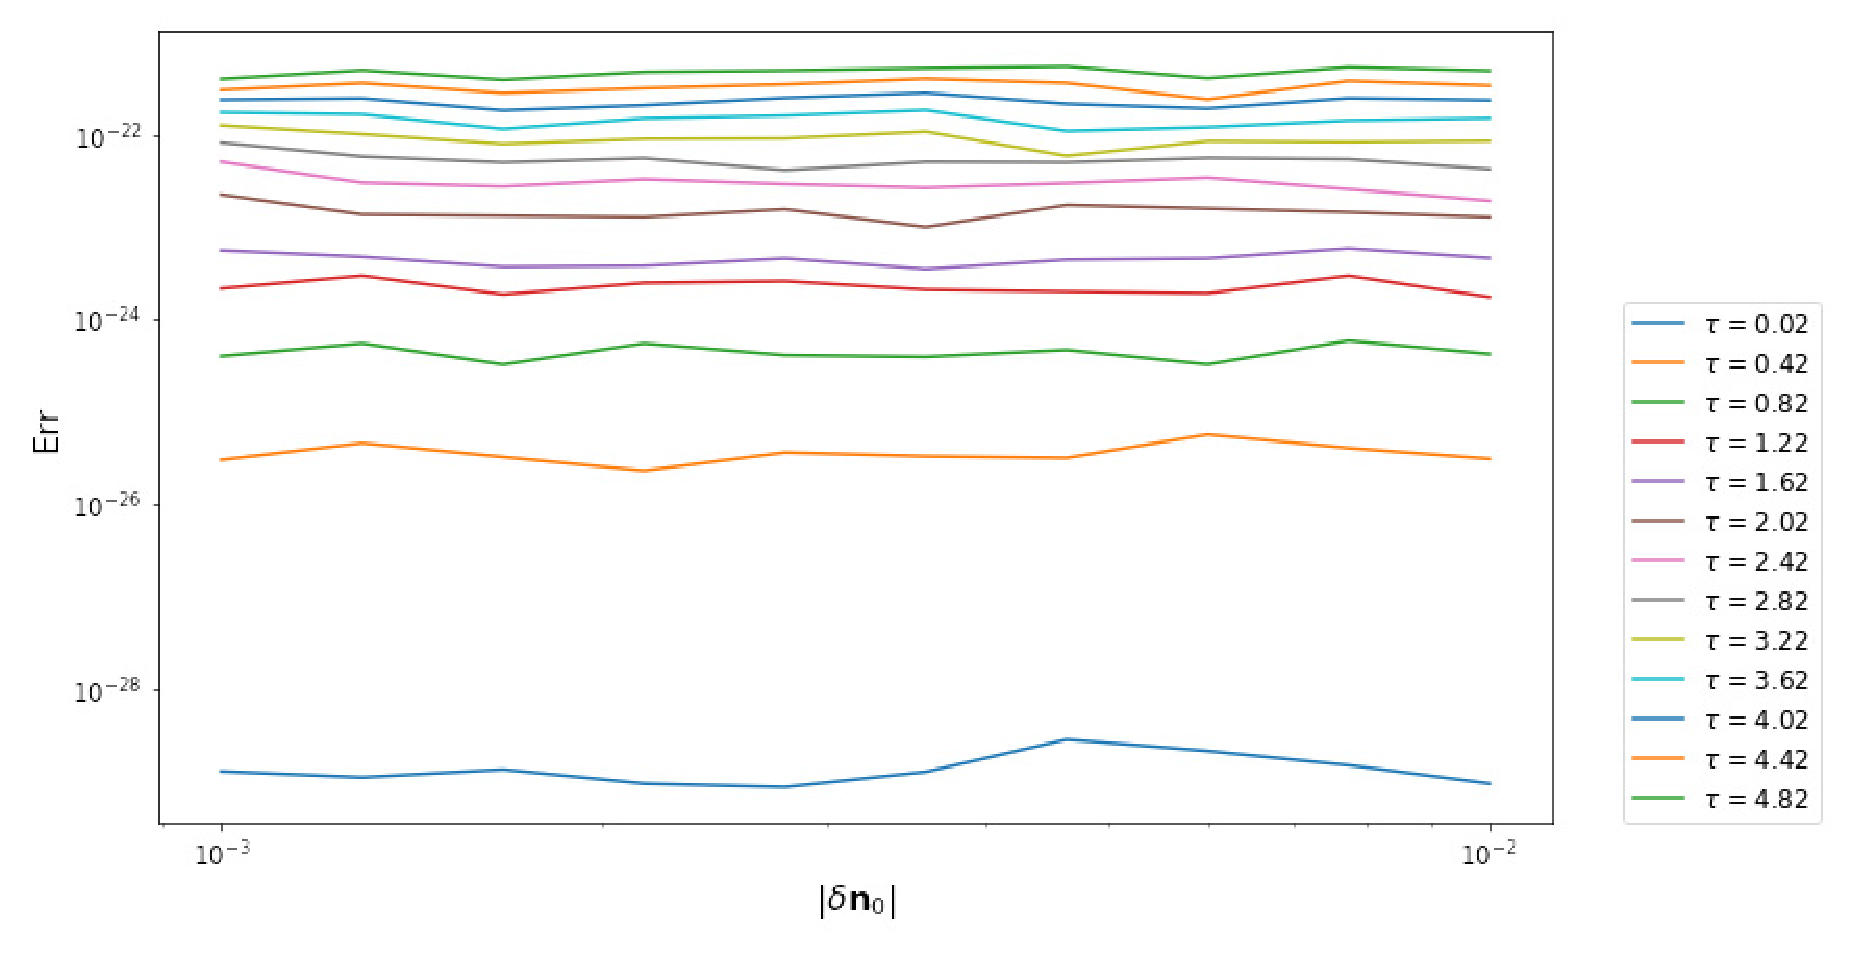
\includegraphics[width=1.0\linewidth]{errline_const.eps}
\caption{Верхние огибающие для нормы ошибки для различных норм $\dn_0$ в заданные моменты времени $\tau$.}
\label{fig:errline_const}
\end{figure}

\noindentИз рис. \ref{fig:errline_const} видно, что максимальная норма ошибки растет со временем, однако рост замедляется. Также для данного поля скоростей характерно равномерное распределение величины ошибки для всех значений $\|\dn_0\|$. 

\noindentИсходя из этого можно сделать вывод, что максимальная норма ошибки на несколько порядков меньше нормы отклонения и вычисления стабильны и не превышает погрешности вычислений.\\

Дополнительно рассмотрим распределения максимумов нормы ошибки на сфере. Для большей наглядности приведем проекцию на плоскость $XY$. Полное изображение для сферы можно посмотреть в приложении.
\begin{figure}[H] 
\centering
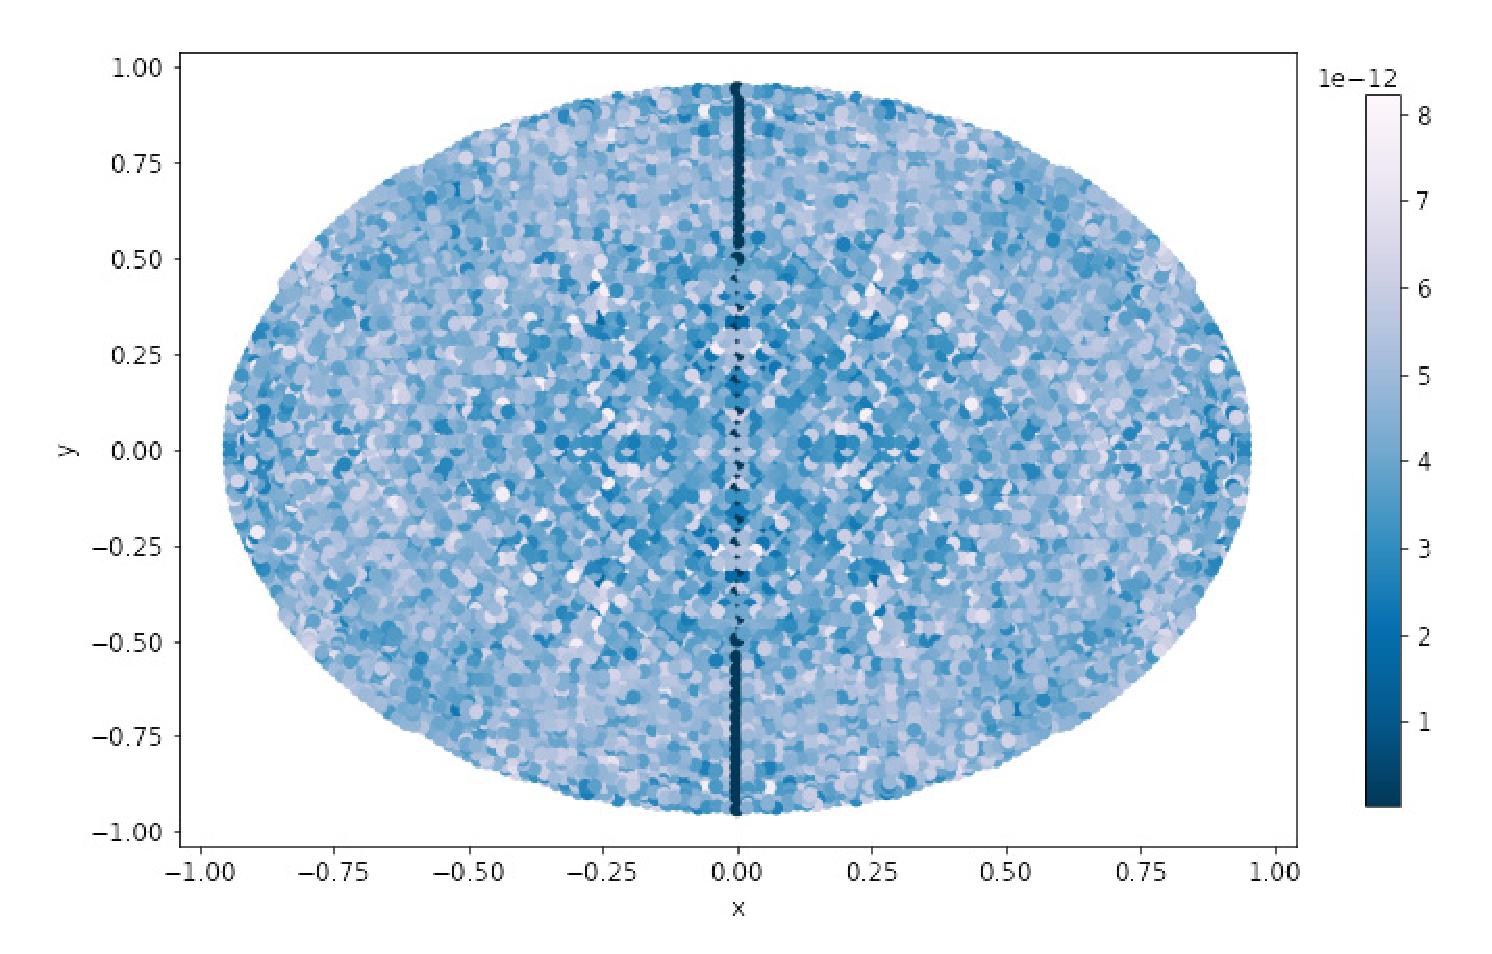
\includegraphics[width=1.0\linewidth]{proj_grad_const.eps}
\caption{Проекция распределения максимальных норм ошибки для различных $\bfv{n}$ и норм $\dn_0$ в заданные моменты времени $\tau = 2.5$\,с.}
\label{fig:proj_grad_const}
\end{figure}

\noindentИз данного распределения можно сделать вывод, что норма ошибки равномерно распределена по начальным направлениям. Наблюдаемая особенность вдоль плоскость $YZ$ вызвана выбором начального смещения $\dn$.\\


\subsubsection{Линейное поле скоростей}
Теперь рассмотрим линейное поле скоростей:
\begin{equation*}
    v(\bfv{r}) = a + b\,\bfv{r}_z, \quad \forall \ \bfv{r} \in R
\end{equation*}

\noindentТогда:
\begin{align*}
\dv{\bfv{r}} &= \T{(0,\,0,\,b)}  &   \ddv{\bfv{r}} &= \matr{\O}
\end{align*}

\noindentСледовательно, матрицы $\matr{M}_{11}$, $\matr{M}_{12}$, $\matr{M}_{21}$ и $\matr{M}_{22}$ системы \eqref{eq:18} примут следующий вид:
\begin{align*} 
&\matr{M}_{11}(\tau) = \begin{bmatrix}
0 & 0 & b\,n_x\\
0 & 0 & b\,n_y\\
0 & 0 & b\,n_z
\end{bmatrix}&\matr{M}_{12}(\tau) = \begin{bmatrix}
a + b\,r_x & 0 & 0\\
0 & a + b\,r_y & 0\\
0 & 0 & a + b\,r_z
\end{bmatrix}\\\\
&\matr{M}_{21}(\tau) = \begin{bmatrix}
0 & 0 & 0\\
0 & 0 & 0\\
0 & 0 & 0
\end{bmatrix}&\matr{M}_{22}(\tau) = \begin{bmatrix}
b\,n_z & 0 & b\,n_x\\
0 & b\,n_z & b\,n_y\\
0 & 0 & 2\,b\,n_z
\end{bmatrix}
\end{align*}

\noindentВ результате получим следующую систему:
\begin{equation} \label{eq:43}
\begin{cases}
\dd{\matr{P}} = \matr{M}_{11}(\tau)\,\matr{P} + \matr{M}_{12}(\tau)\,\matr{Q}\\
\dd{\matr{Q}} = \matr{M}_{22}(\tau)\,\matr{Q}\\
\matr{P}|_{\tau=0} = \matr{\O}; \ \matr{Q}|_{\tau=0} = \matr{I}
\end{cases}
\end{equation}

\noindentЛегко видеть, что решение первого уравнения зависит от решения второго, однако решение второго не зависит от первого. Следовательно, система распадается на две системы из трех дифференциальных уравнений (в силу того, что матрицы $\matr{M}_{12}$ и $\matr{M}_{22}$ полного ранга), решаемых последовательно.

\begin{align*}
\begin{cases}
\dd{\matr{Q}} = \matr{M}_{22}(\tau)\,\matr{Q}\\
\matr{Q}|_{\tau=0} = \matr{I}
\end{cases}   
\quad & \quad   
\begin{cases}
\dd{\matr{P}} = \matr{M}_{11}(\tau)\,\matr{P} + \matr{M}_{12}(\tau)\,\matr{Q}\\
\matr{P}|_{\tau=0} = \matr{0}
\end{cases} 
\end{align*}

Положим для теста $a = 500$\,м/с, $b = -10$\,$\text{с}^{-1}$ и рассмотрим численные значения норм отклонений \eqref{eq:41} для различных моментов времени.

\begin{figure}[H] 
\centering
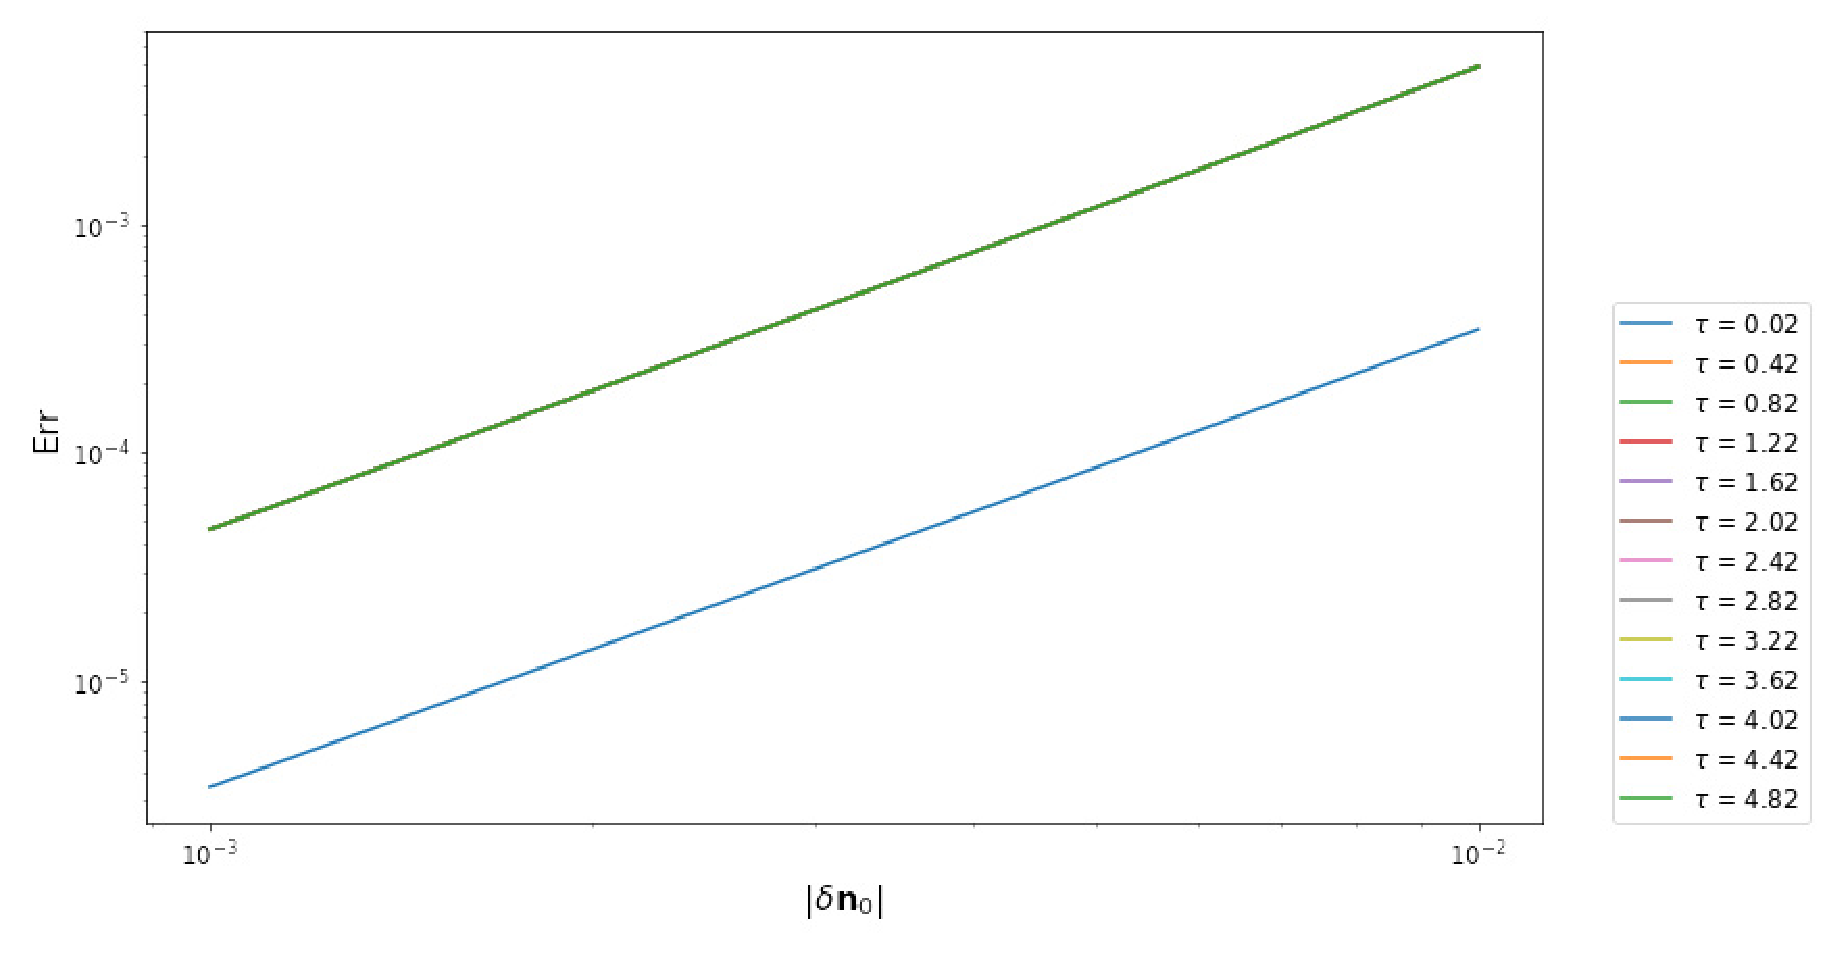
\includegraphics[width=1.0\linewidth]{errline_lin.eps}
\caption{Верхние огибающие для нормы ошибки для различных норм $\dn_0$ в заданные моменты времени $\tau$.}
\label{fig:errline_lin}
\end{figure}

\noindentИз рис. \ref{fig:errline_lin} можно видеть, что норма ошибки имеет порядок нормы отклонения. Абсолютное значение отклонения имеет значение порядка $10^{-3}-10^{-2}$\,м. Также интересной особенностью является стабилизация максимальной нормы ошибки начиная с $\tau = 0.2$\,с.\\

Рассмотрим, как и в первом случае, распределение максимумов норм ошибки на сфере. Для большей наглядности приведем проекцию на плоскость $XY$. Полное изображение для сферы также можно найти в приложении.
\begin{figure}[H] 
\centering
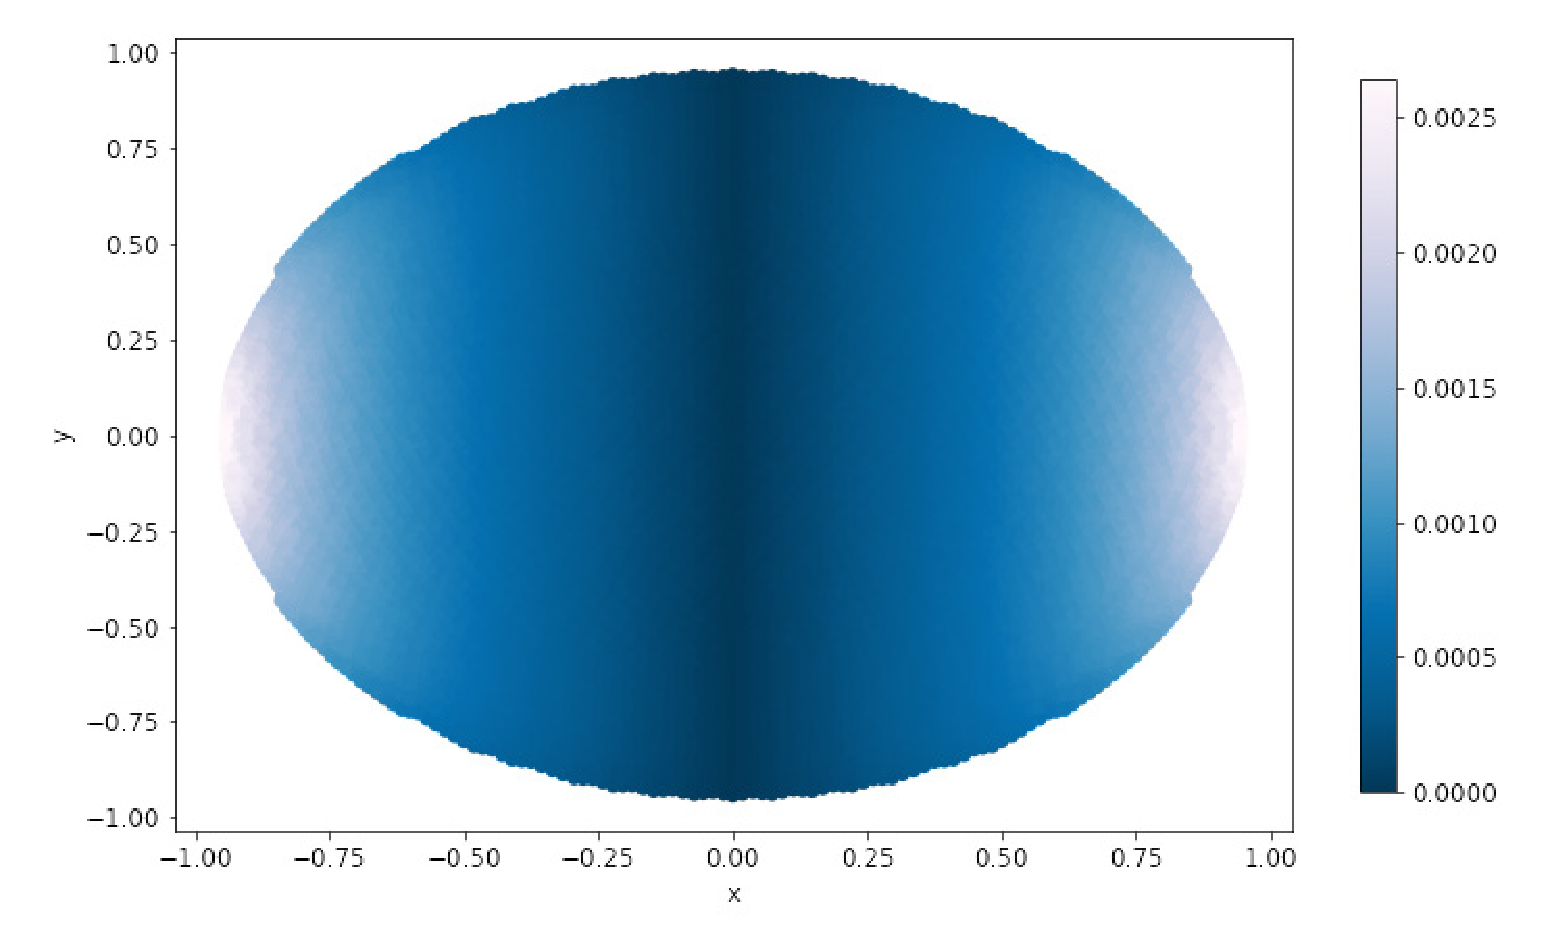
\includegraphics[width=1.0\linewidth]{proj_grad_lin.eps}
\caption{Проекция максимальные нормы ошибки для различных $\bfv{n}$ и норм $\dn_0$ в заданные моменты времени $\tau = 1.6$\,с.}
\label{fig:proj_grad_lin}
\end{figure}

\noindentДля данного распределения наблюдается увлечение ошибки при приближении к краям волнового фронта вдоль направления, параллельного заданному полю скоростей. Особенность вдоль оси $YZ$, как и в первом случае, сохраняется.\\


\subsubsection{Модельное поле скоростей}
Рассмотрим численные значения норм отклонений \eqref{eq:41} для различных моментов времени.
\begin{figure}[H] 
\centering
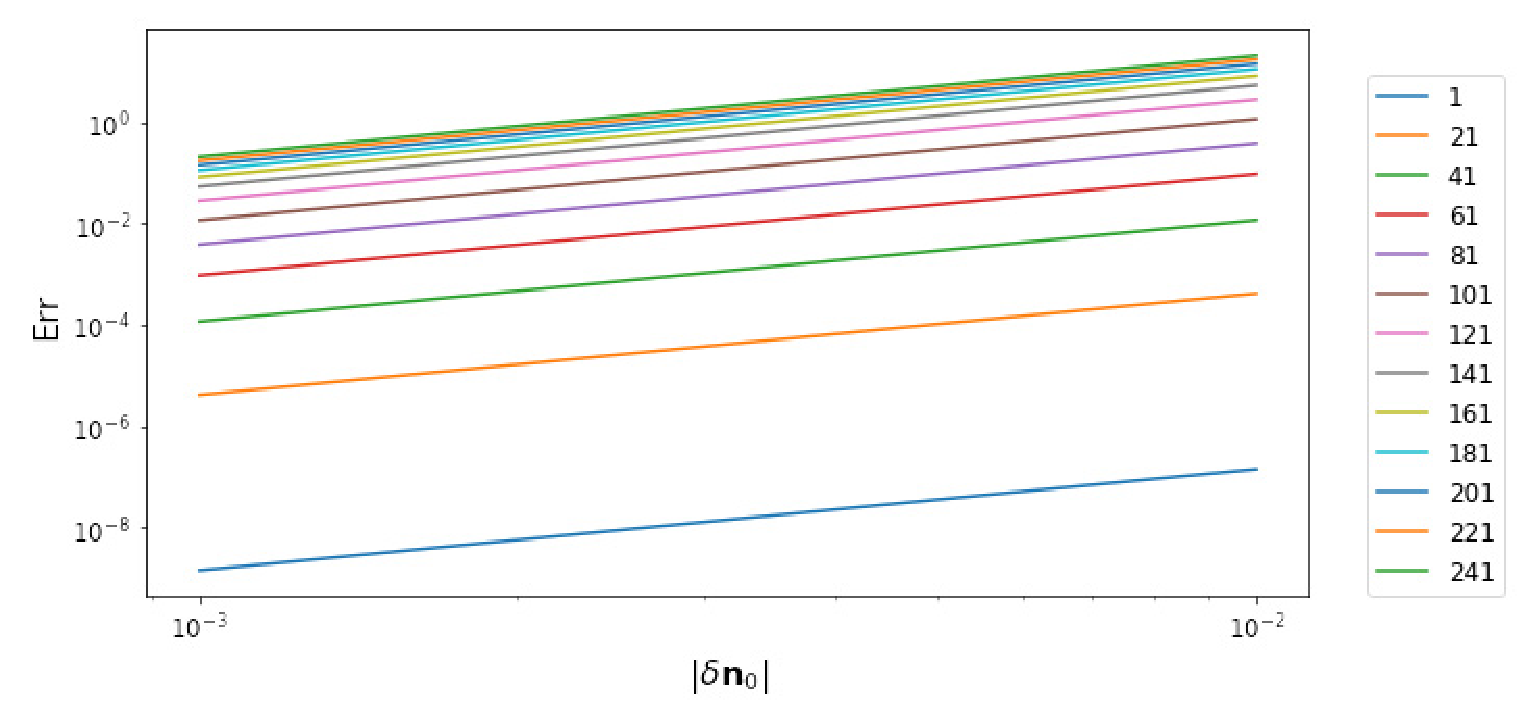
\includegraphics[width=1.0\linewidth]{errline_gauss.eps}
\caption{Верхние огибающие для нормы ошибки для различных норм $\dn_0$ в заданные моменты времени $\tau$.}
\label{fig:errline_gauss}
\end{figure}

\noindentНорма ошибки для данного распределения скоростей выше, чем у ранее рассмотренных, и на два порядка выше нормы отклонения. Однако его абсолютное значение не превышает $1-10$\,м.\\

\noindentАналогично предыдущим пунктам рассмотрим проекцию распределения максимумов норм ошибки на сфере. Полное изображение для сферы приведено в приложении.
\begin{figure}[H] 
\centering
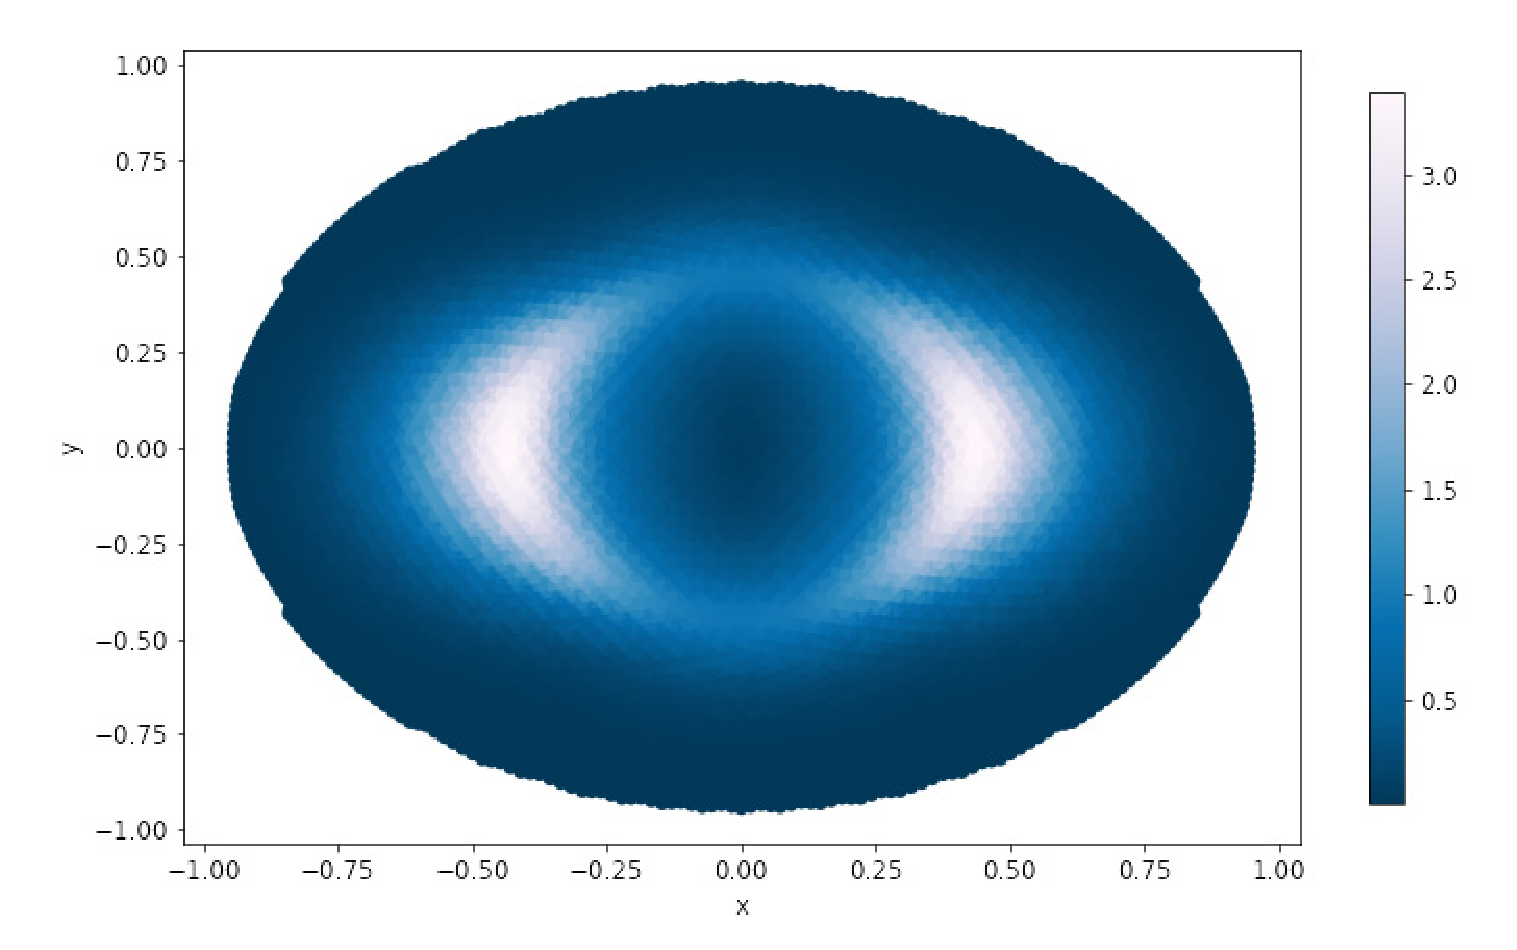
\includegraphics[width=1.0\linewidth]{proj_grad_gauss.eps}
\caption{Проекция максимальные нормы ошибки для различных $\bfv{n}$ и норм $\dn_0$ в заданные моменты времени $\tau = 1.6$\,с.}
\label{fig:proj_grad_gauss}
\end{figure}

\noindentДля данного распределения наблюдается увлечение ошибки на шаровом поясе. Особенность вдоль оси $YZ$, как и ранее, сохраняется. В основной массе направлений абсолютная норма ошибки имеет порядок меньше 1\,м.\\

\subsection{Решение прямой задачи}
Продемонстрируем результат работы алгоритма решения прямой задачи для модельного поля скоростей. Волновой фронт для него содержит характерные каустики, по которым можно судить о работоспособности решения. Для наглядности будем рассматривать срез вдоль плоскости $y = 0$ совокупности фронтов для различных $\tau$. Также приведем вид волнового фронта для момента времени $\tau = 5$\,с.
\begin{figure}[H] 
\centering
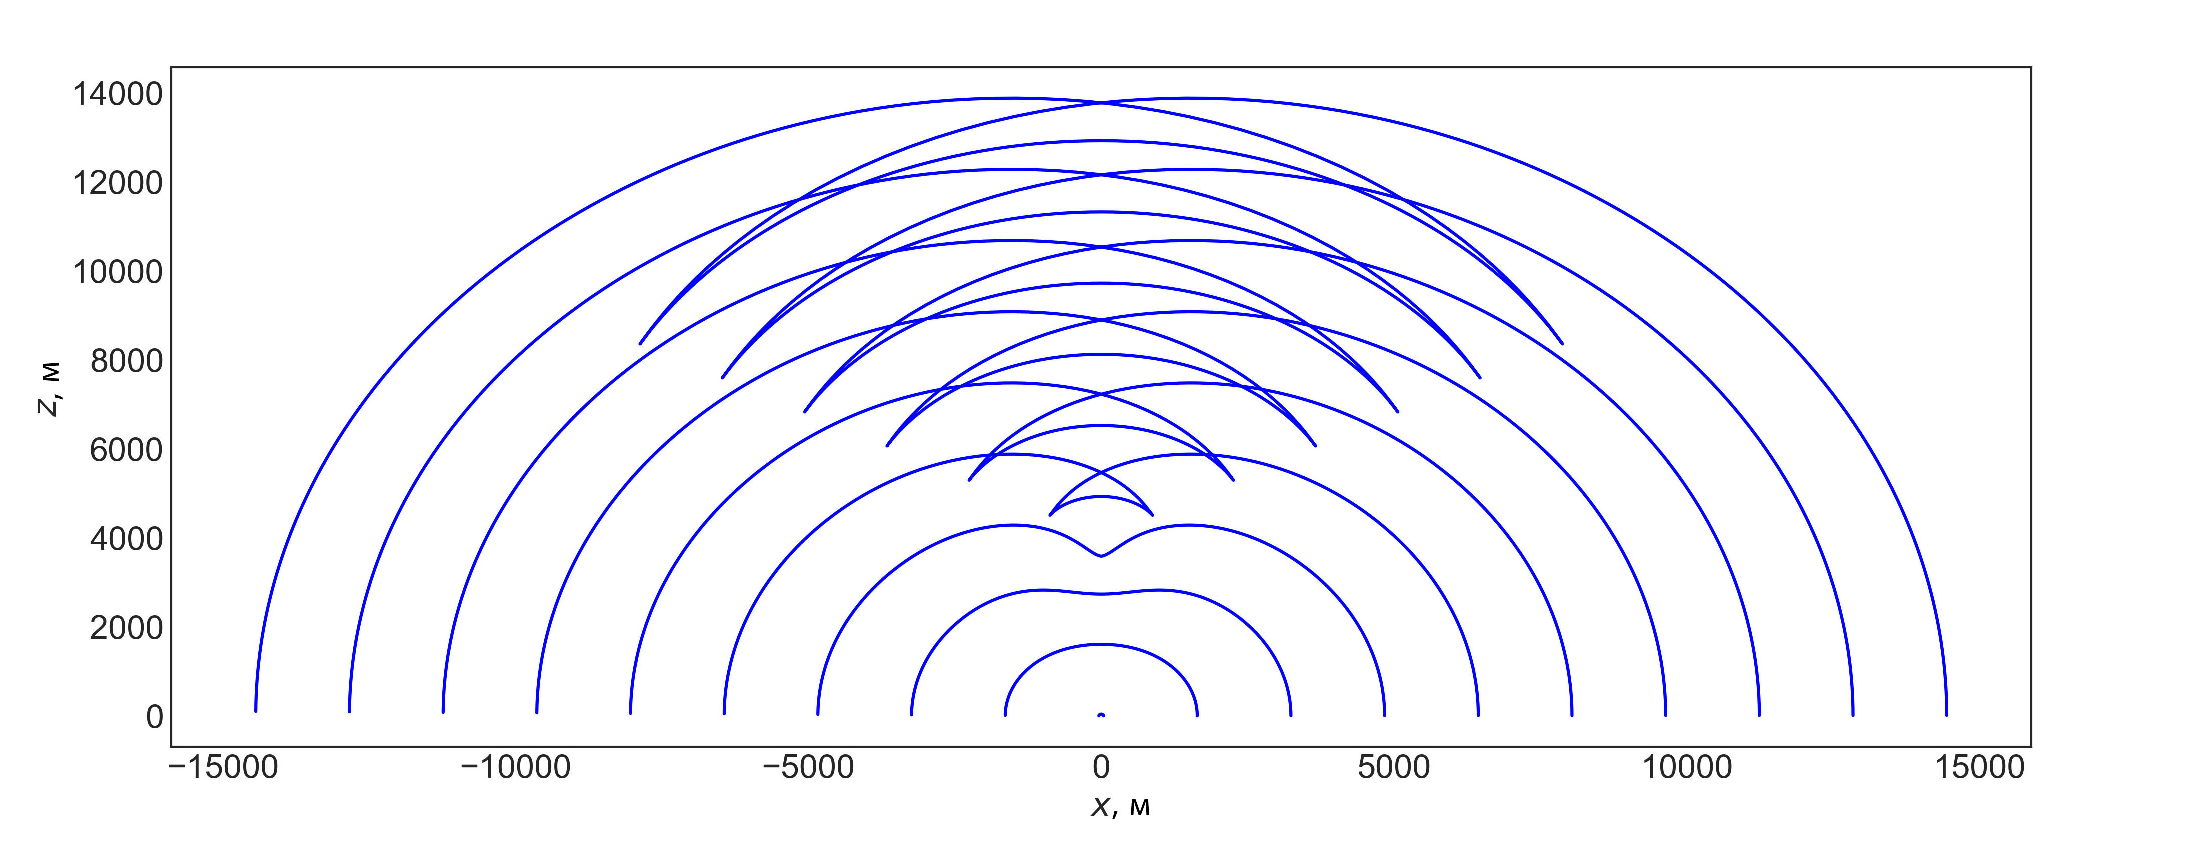
\includegraphics[width=1.0\linewidth]{direct_problem2d.eps}
\caption{Двумерная проекция волнового фронта при $y = 0$.}
\label{fig:direct_problem2d}
\end{figure}

\begin{figure}[H] 
\centering
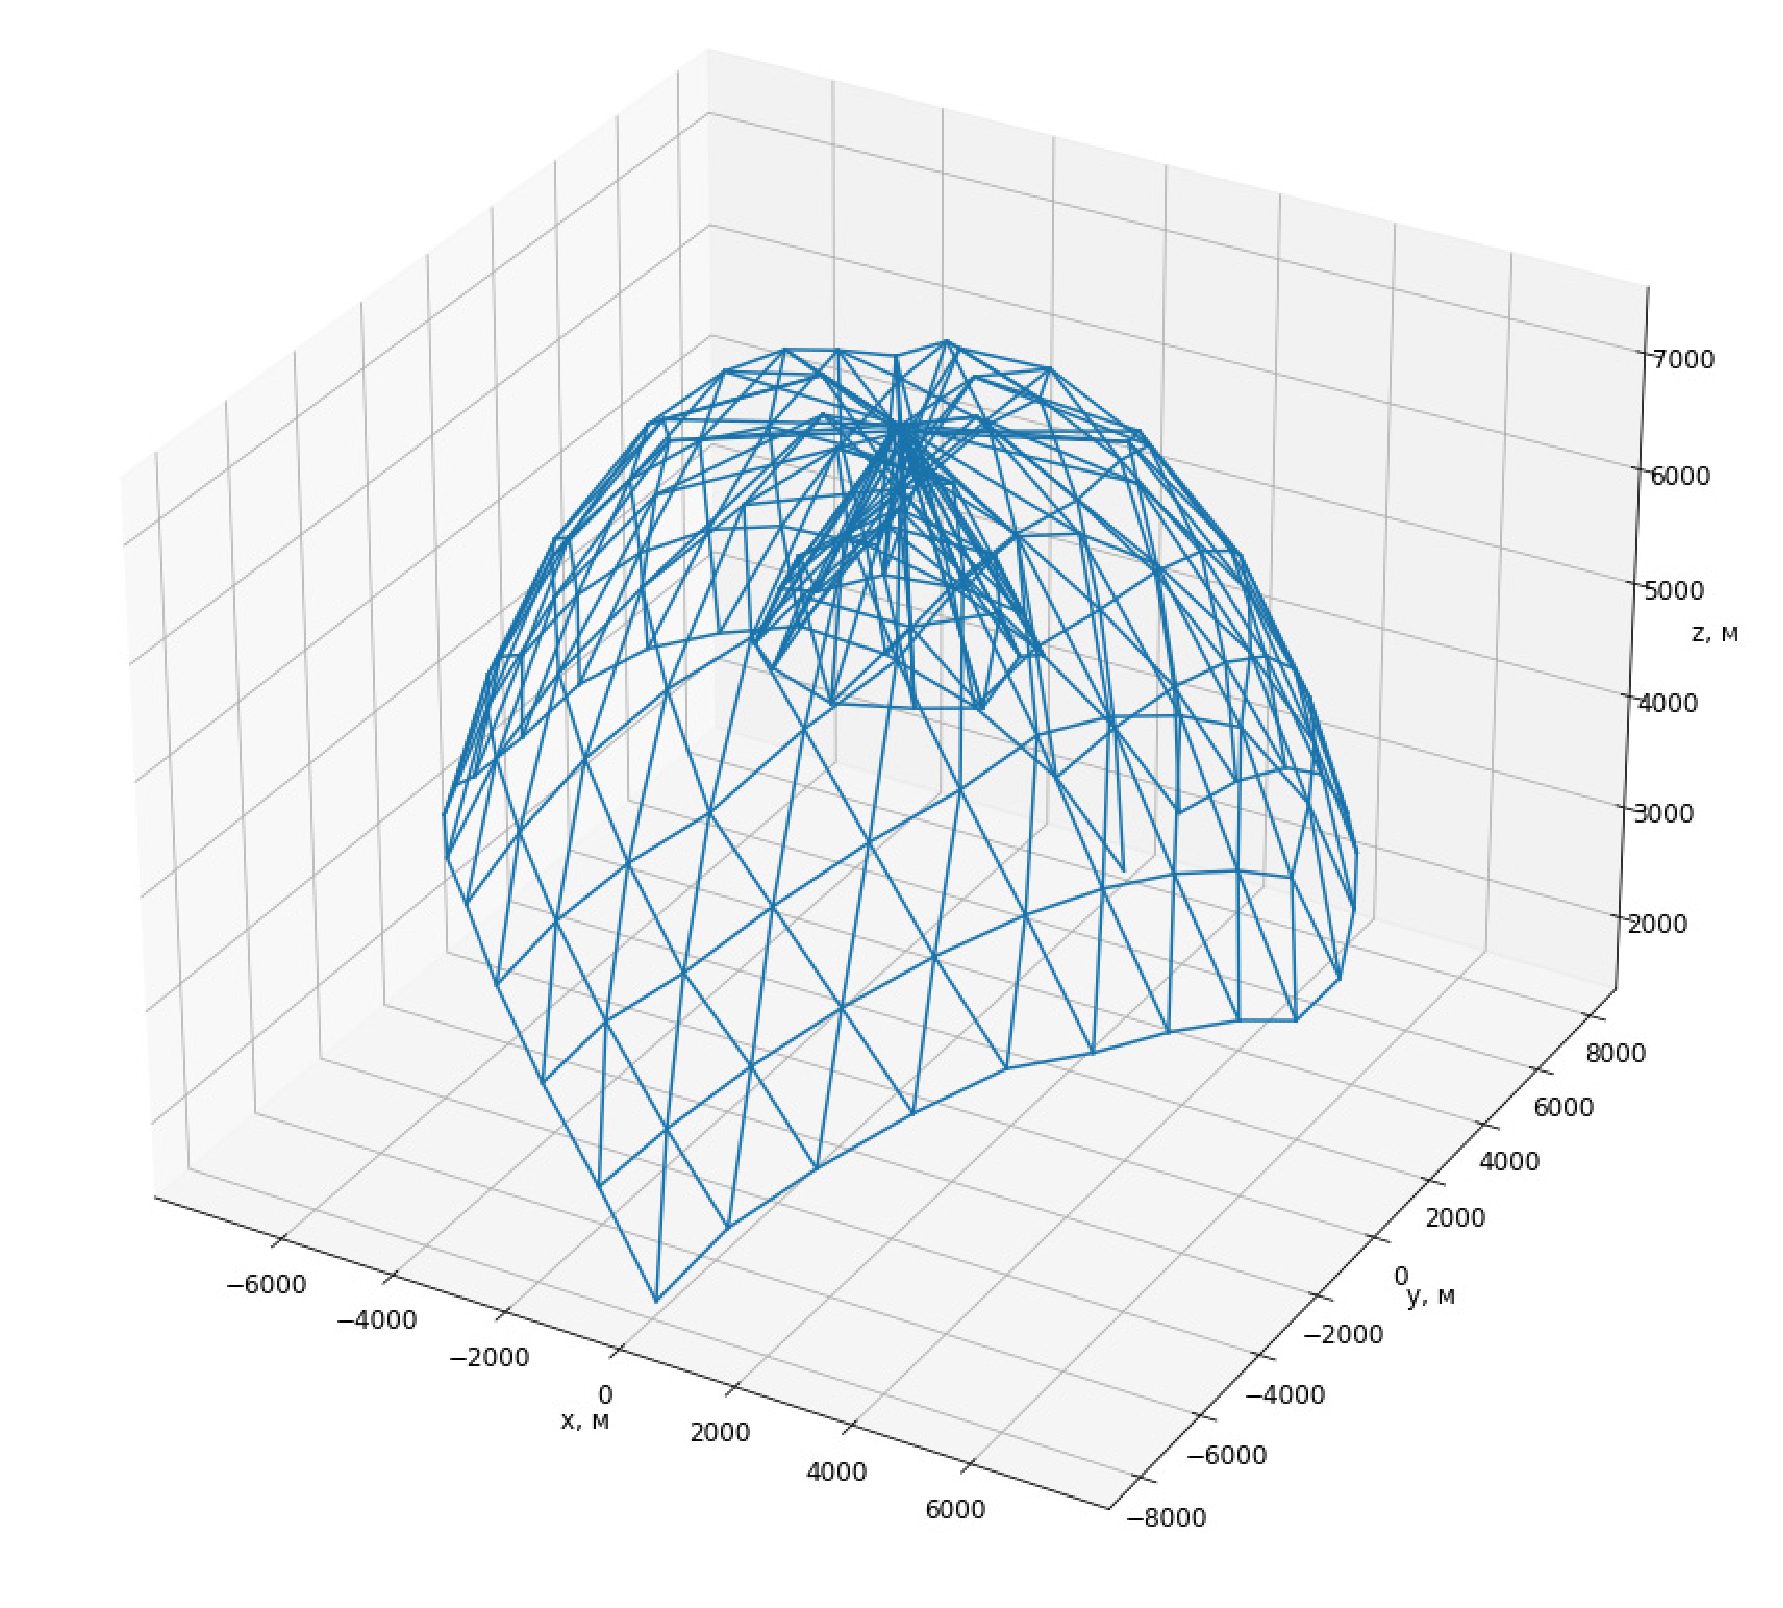
\includegraphics[width=1.0\linewidth]{direct_problem3d.eps}
\caption{Волновой фронт при решении прямой задачи в момент времени $\tau = 4$\,с.}
\label{fig:direct_problem3d}
\end{figure}

\noindentНа рис. \ref{fig:direct_problem2d} действительно наблюдаются характерные каустики, из чего можно сделать вывод, что решение прямой задачи работает верно.

\subsection{Решение обратной задачи простым перебором}
При проверке корректности работы алгоритма решения обратной задачи мы будем отталкиваться от основной сути задачи --- поддержки заданного размера ребер сетки. Для этого рассмотрим зависимость максимальной длины ребра сетки от времени.
\begin{figure}[H] 
\centering
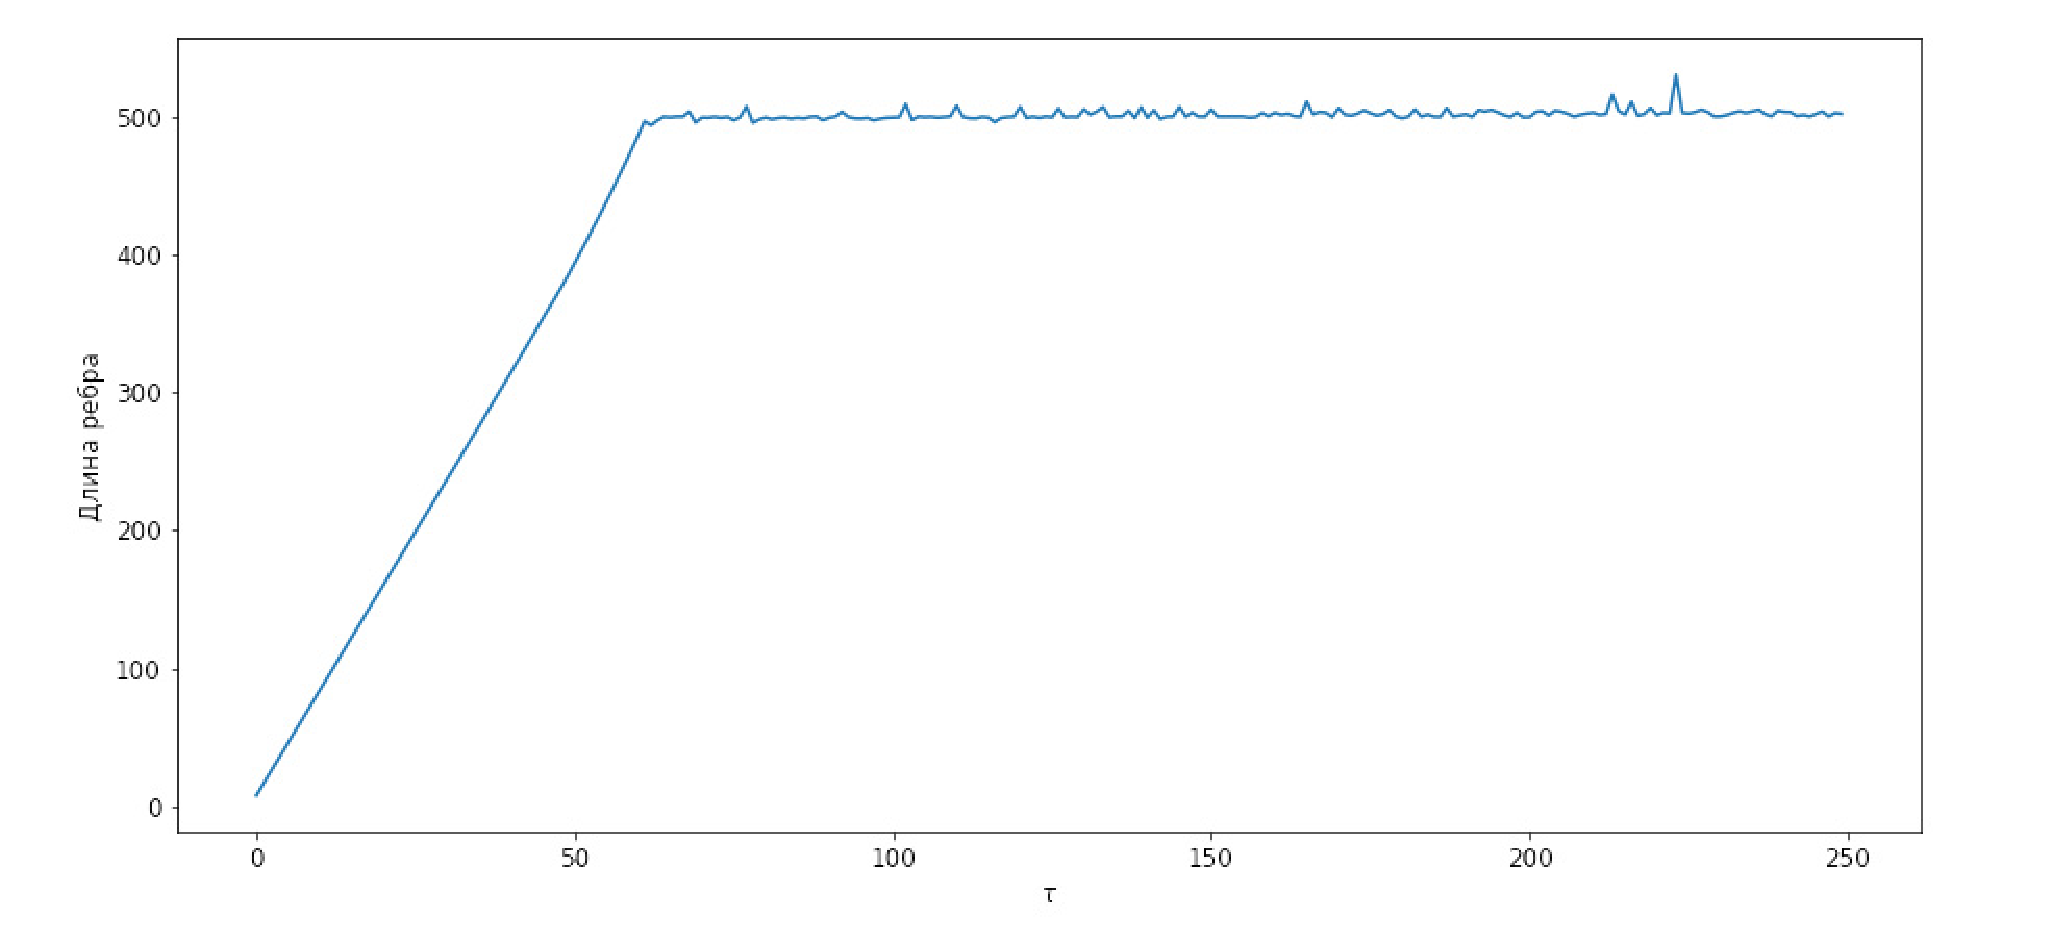
\includegraphics[width=1.0\linewidth]{direct_search_edge_len.eps}
\caption{Зависимость максимальной длины ребра от времени для метода прямого перебора.}
\label{fig:direct_search_edge_len}
\end{figure}

\noindentКак можно видеть из рис. \ref{fig:direct_search_edge_len}, максимальная длина ребра находится, в целом, удовлетворяет ограничениям в 500\,м, что подтверждает корректность решения задачи.


\subsection{Решение обратной задачи градиентным спуском}
Также как и ранее, рассмотрим зависимость максимальной длины ребра сетки от времени.
\begin{figure}[H] 
\centering
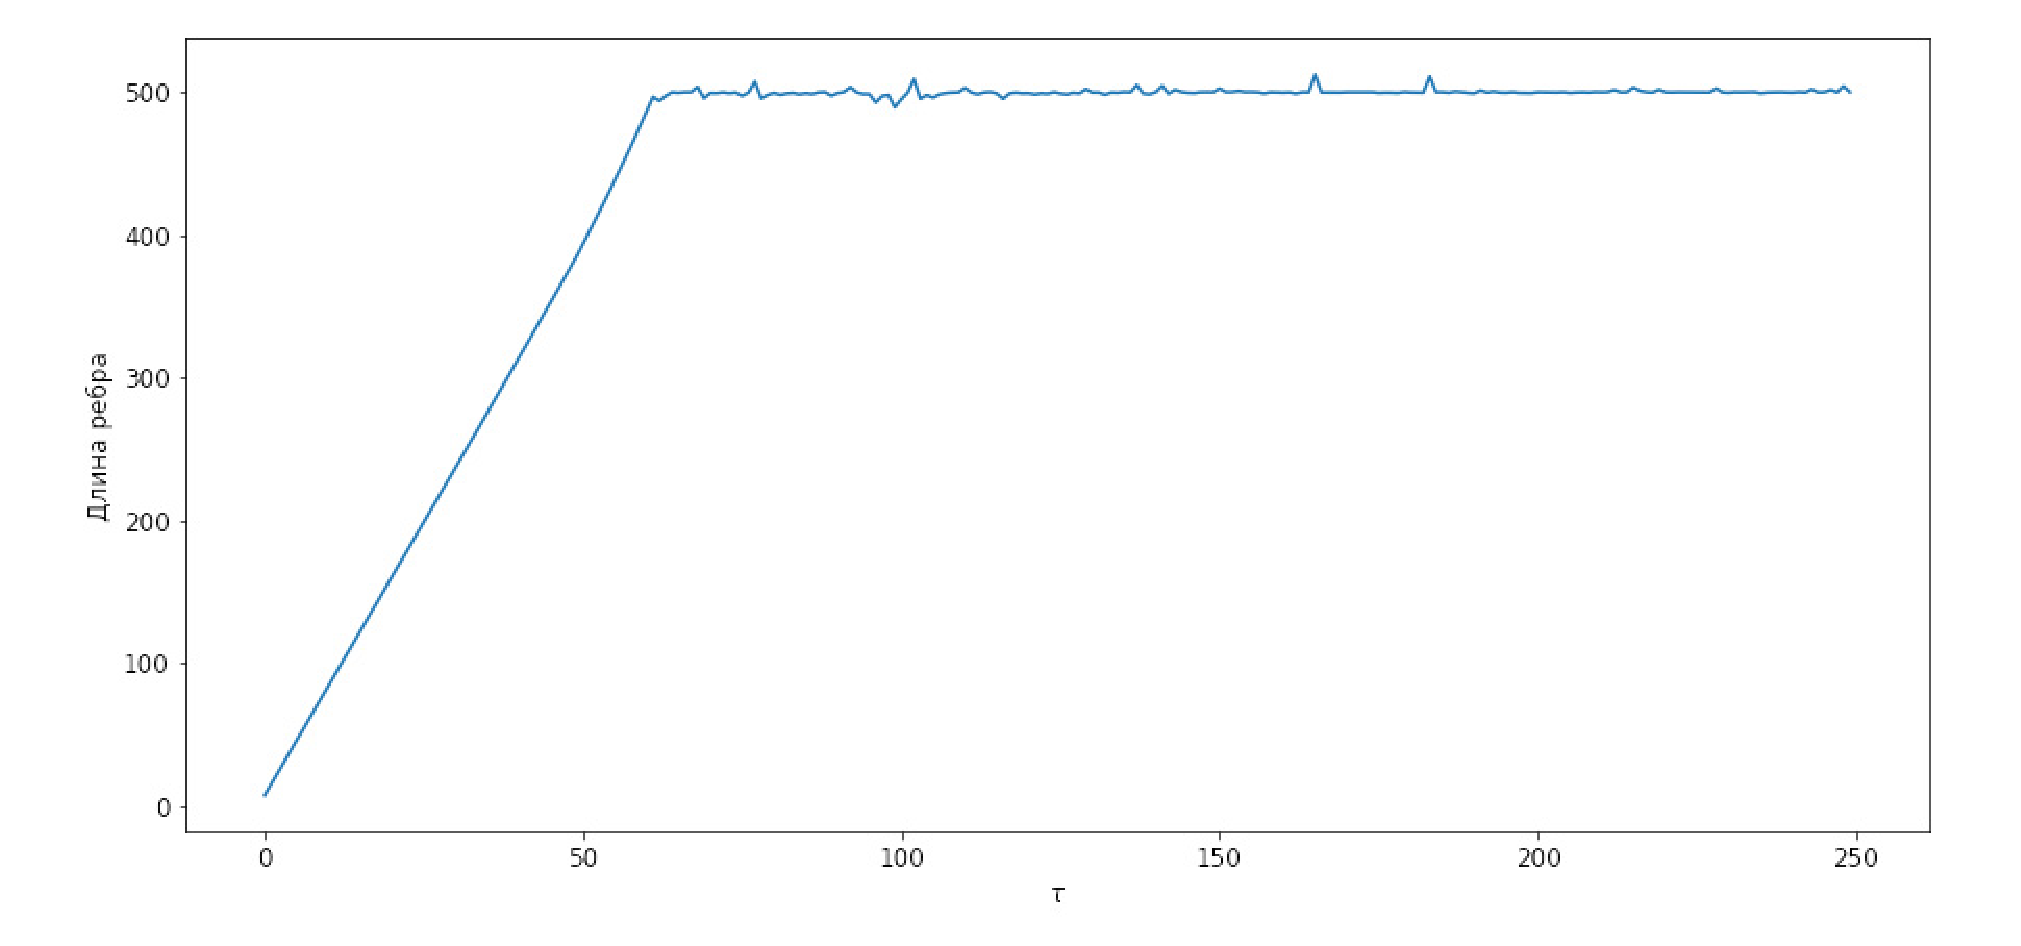
\includegraphics[width=1.0\linewidth]{grad_step_edge_len.eps}
\caption{Зависимость максимальной длины ребра от времени.}
\label{fig:grad_step_edge_len}
\end{figure}

\noindentКак можно видеть из рис. \ref{fig:direct_search_edge_len}, максимальная длина ребра также находится в заданных пределах, что подтверждает корректность решения задачи.

\subsection{Решение обратной задачи градиентным спуском с импульсом}
Рассмотрим зависимость максимальной длины ребра сетки от времени.
\begin{figure}[H] 
\centering
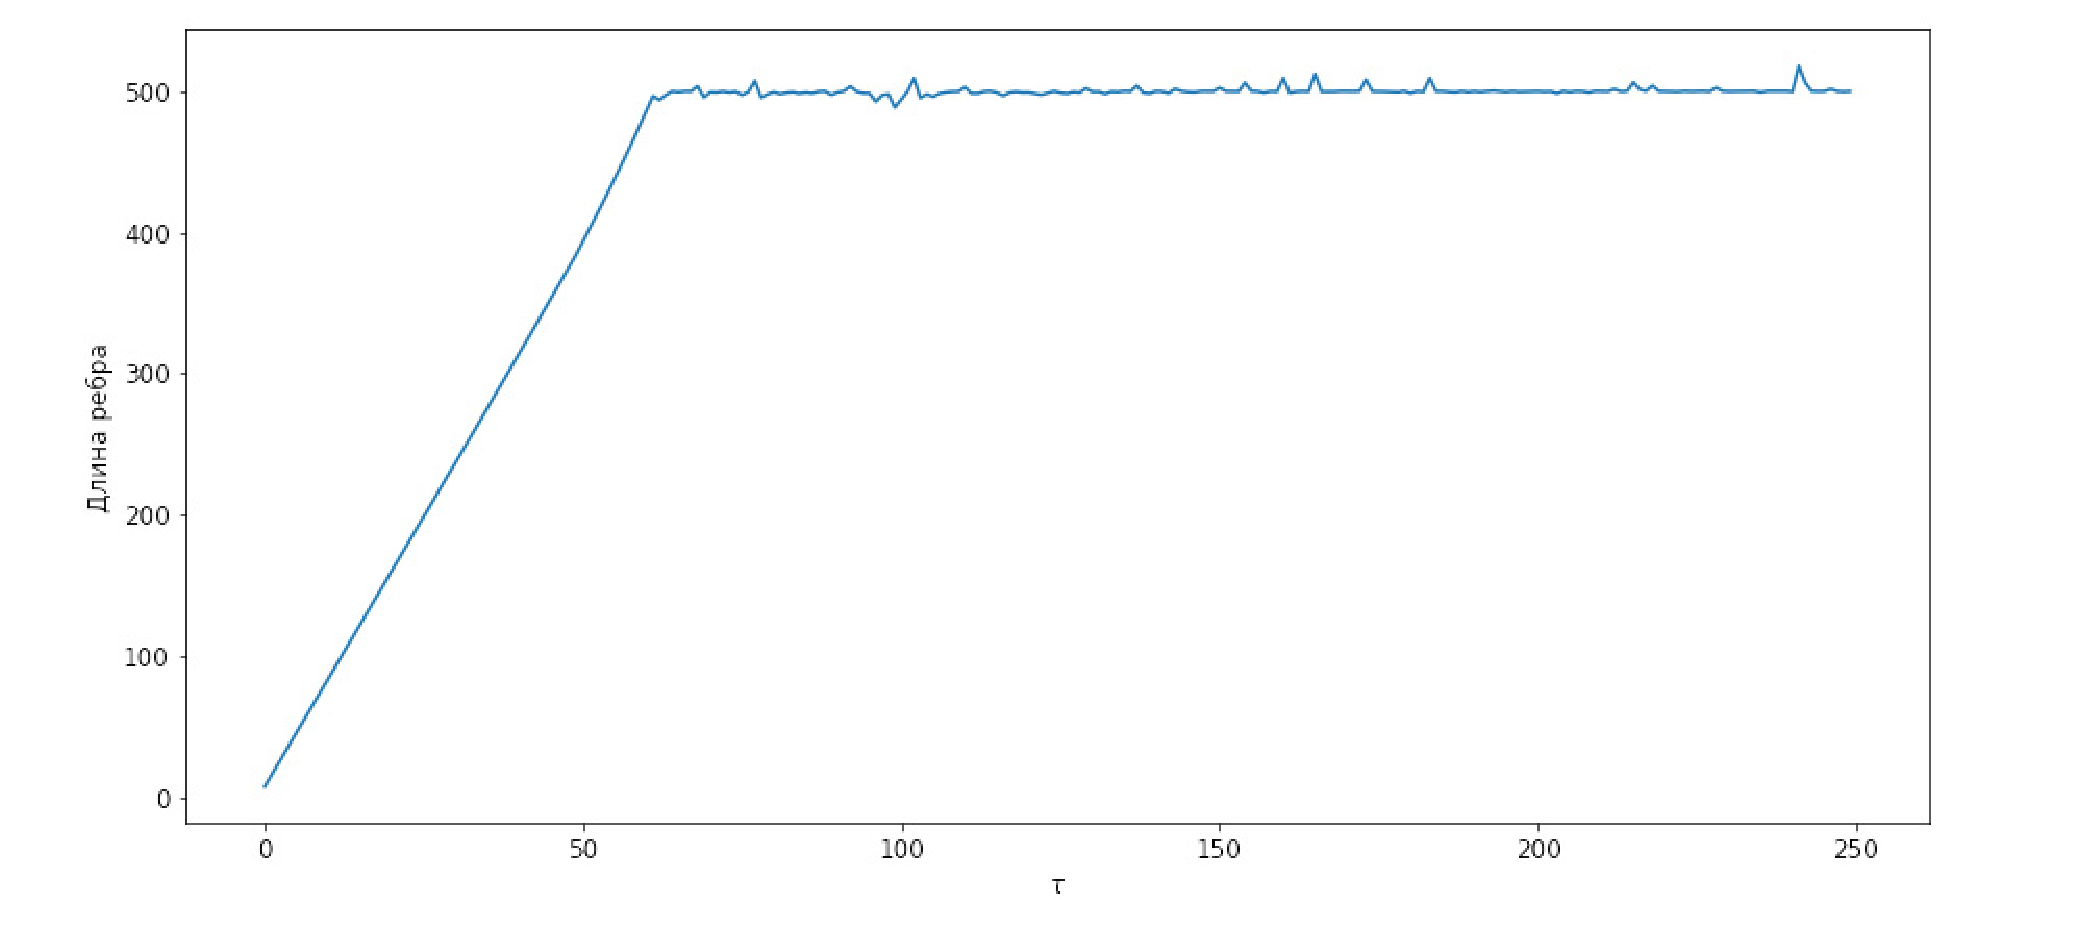
\includegraphics[width=1.0\linewidth]{grad_impulse_edge_len.eps}
\caption{Максимальные нормы ошибки для различных $\bfv{n}$ и норм $\dn_0$ в заданные моменты времени $\tau = 1.6$\,с.}
\label{fig:grad_impulse_edge_len}
\end{figure}

\noindentИз рис. \ref{fig:direct_search_edge_len} видно, что максимальная длина ребра находится в заданных пределах, что подтверждает корректность решения задачи.

\subsection{Оценки сложности алгоритмов решение обратной задачи}
Основная вычислительная сложность решения обратной задачи заключается в трассировках множества лучей сетки, а также дополнительных лучей, возникающих в следствии поиска оптимального положения конца добавляемого луча. В связи с этим, для оценки сложности приведем зависимость количества лучевых трубок от времени для разных методов.
\begin{figure}[H]
\centering
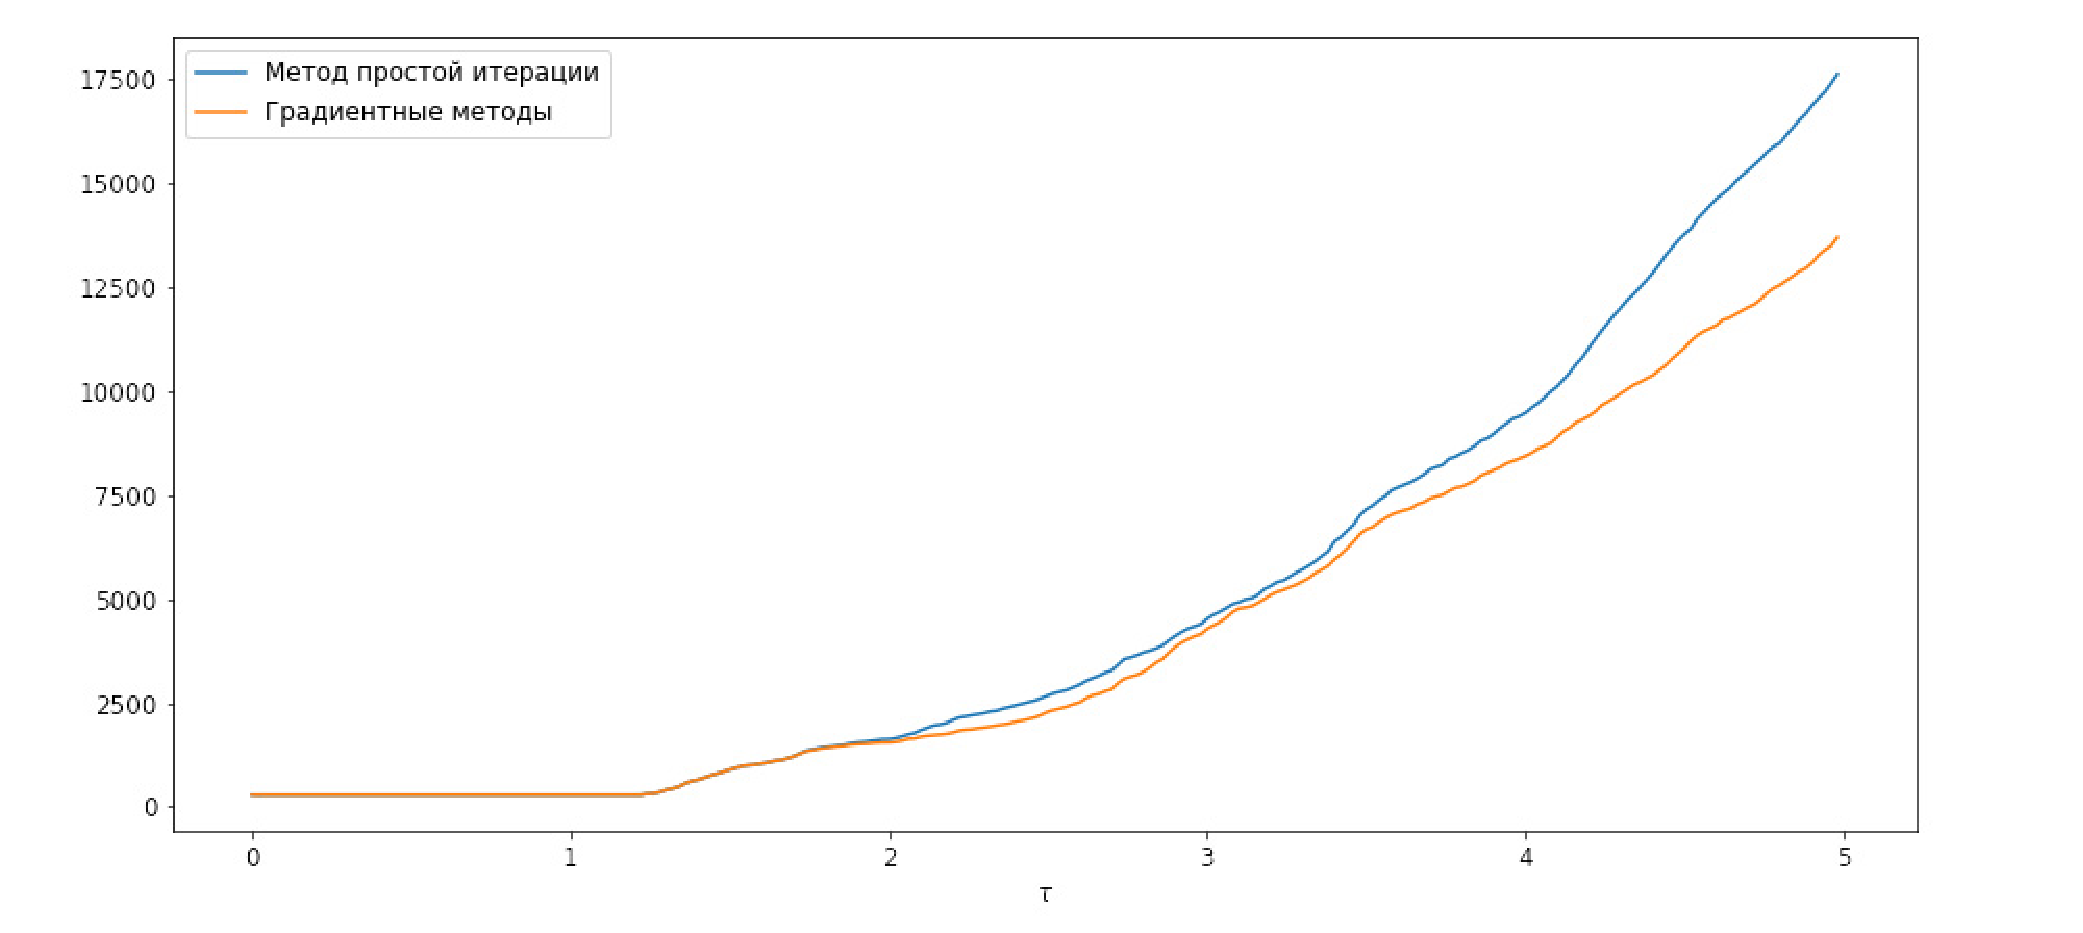
\includegraphics[width=1.0\linewidth]{comp_all_tube.eps}
\caption{Зависимость количества лучевых трубок от времени для рассматриваемых методов.}
\label{fig:comp_all_tube}
\end{figure}

\noindentИз рис. \ref{fig:comp_all_tube} следует, что при решении методом простой итерации приходится чаще добавлять новые лучи в сетку, что говорит о более низкой точности, по сравнению с градиентными методами. Также оба рассматриваемых метода на основе градиентного спуска объединены в одну группу, так как различие в числе трубок у них несущественно. 

Теперь приведем сравнение количества лучевых трубок и дополнительных трассировок, которые требуются алгоритму для работы, для каждого момента времени $\tau$.

\begin{figure}[H]
\centering
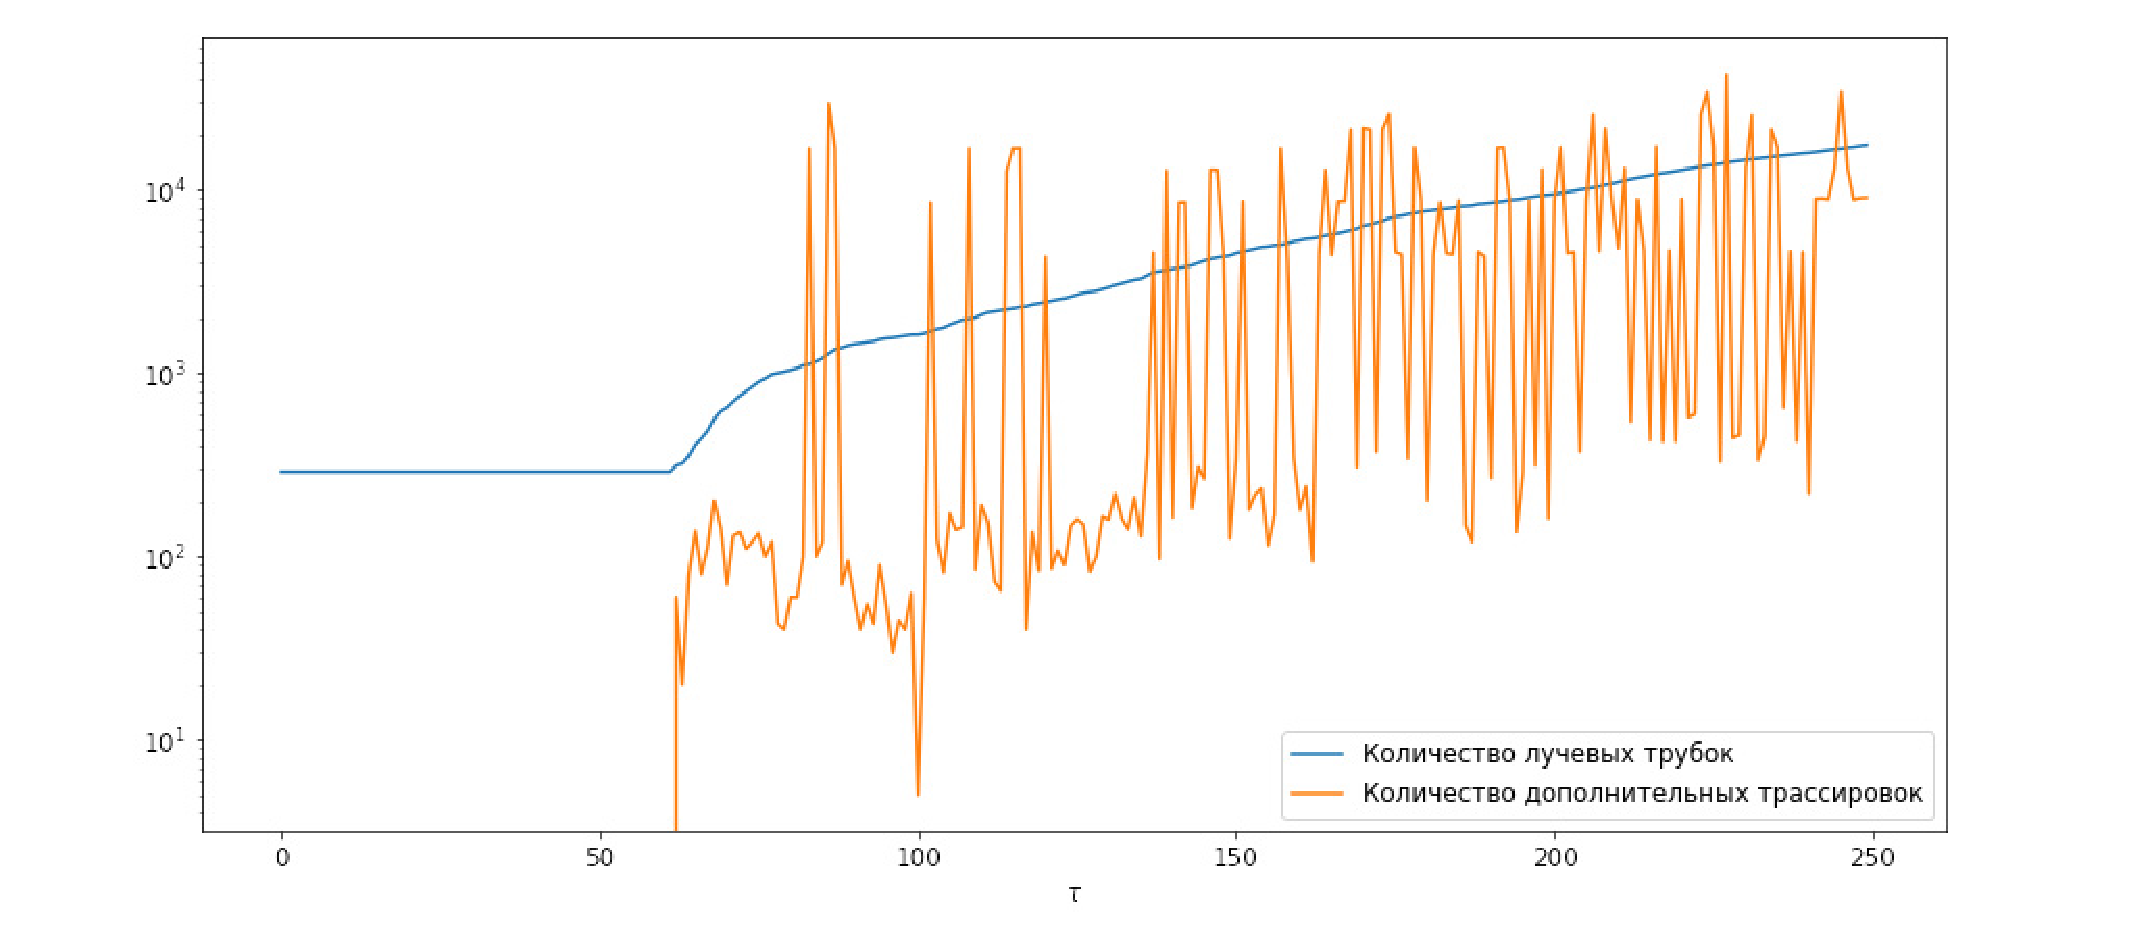
\includegraphics[width=1.0\linewidth]{add_trac_direct_search.eps}
\caption{Количество дополнительных трассировок и лучевых трубок для метода простой итерации.}
\label{fig:add_trac_direct_search}
\end{figure}

\noindentИз рис. \ref{fig:add_trac_direct_search} можно сделать вывод, что количество дополнительных трассировок в среднем не более чем на порядок больше текущего числа лучевых трубок.

\begin{figure}[H] 
\centering
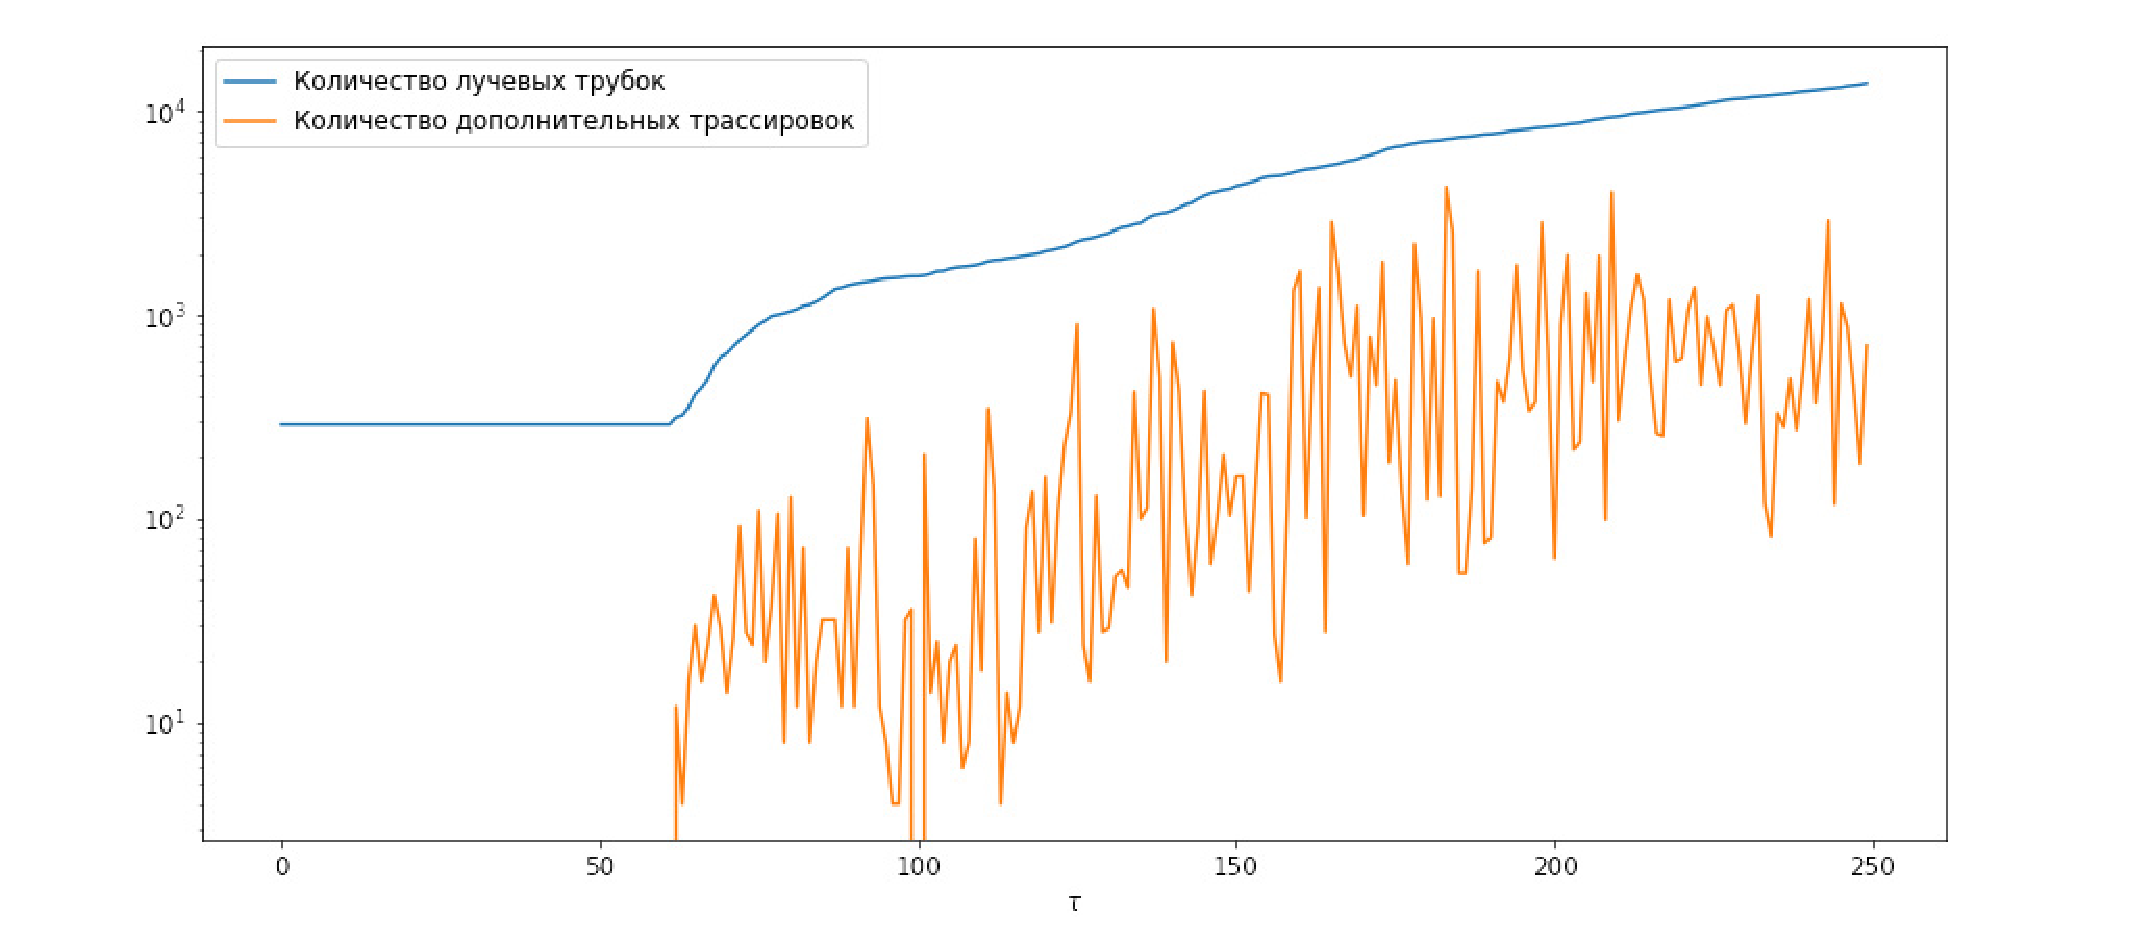
\includegraphics[width=1.0\linewidth]{add_trac_grad_step.eps}
\caption{Количество дополнительных трассировок и лучевых трубок для градиентного спуска.} 
\label{fig:add_trac_grad_step}
\end{figure}

\noindentИз рис. \ref{fig:add_trac_grad_step} можно сделать вывод, что количество дополнительных трассировок в среднем на порядок меньше текущего числа лучевых трубок.

\begin{figure}[H] 
\centering
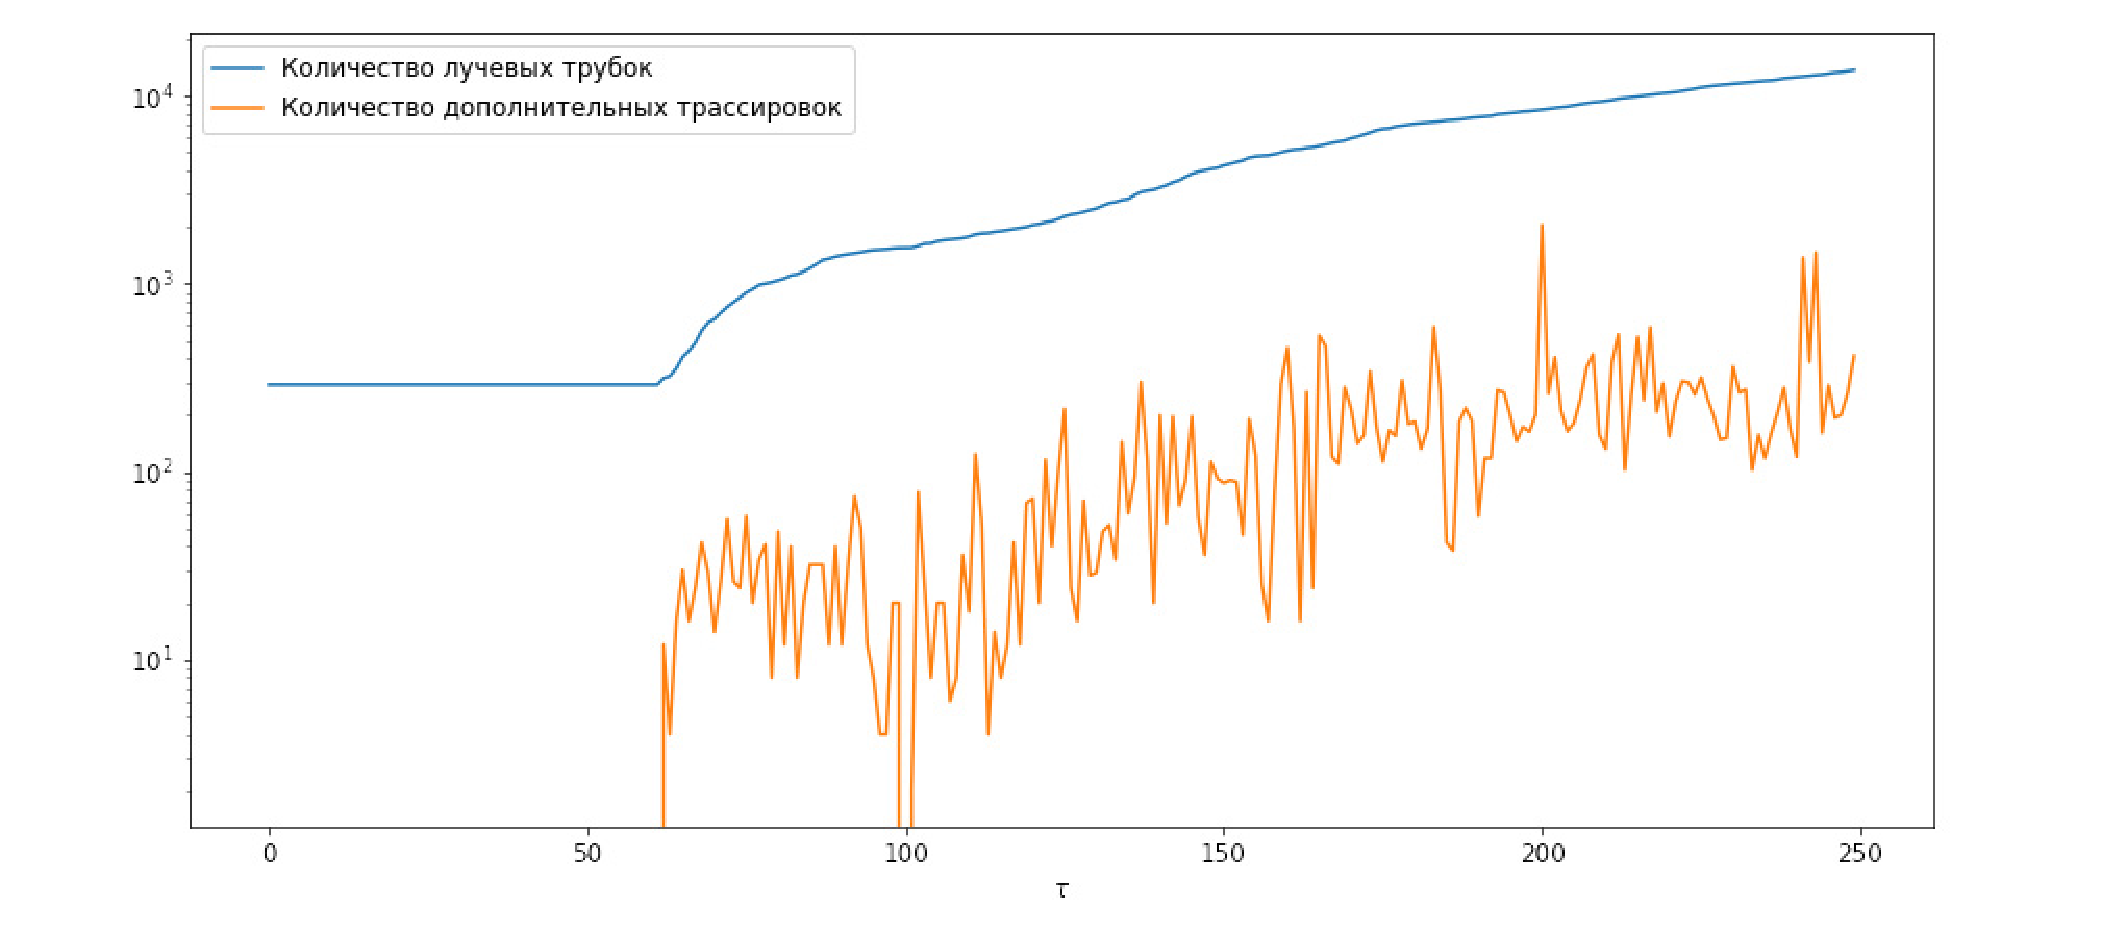
\includegraphics[width=1.0\linewidth]{add_trac_grad_impulse.eps}
\caption{Количество дополнительных трассировок и лучевых трубок для градиентного спуска с импульсом.}
\label{fig:add_trac_grad_impulse}
\end{figure}

\noindentИз рис. \ref{fig:add_trac_grad_impulse} можно сделать вывод, что количество дополнительных трассировок в среднем на полтора порядка меньше текущего числа лучевых трубок.

\noindentИз этого можно сделать вывод, что наибольшую эффективность имеет метод решения обратной задачи с использованием градиентного спуска с импульсом.

Приведем сравнение общего числа дополнительных трассировок на каждом шаге для методов.

\begin{figure}[H] 
\centering
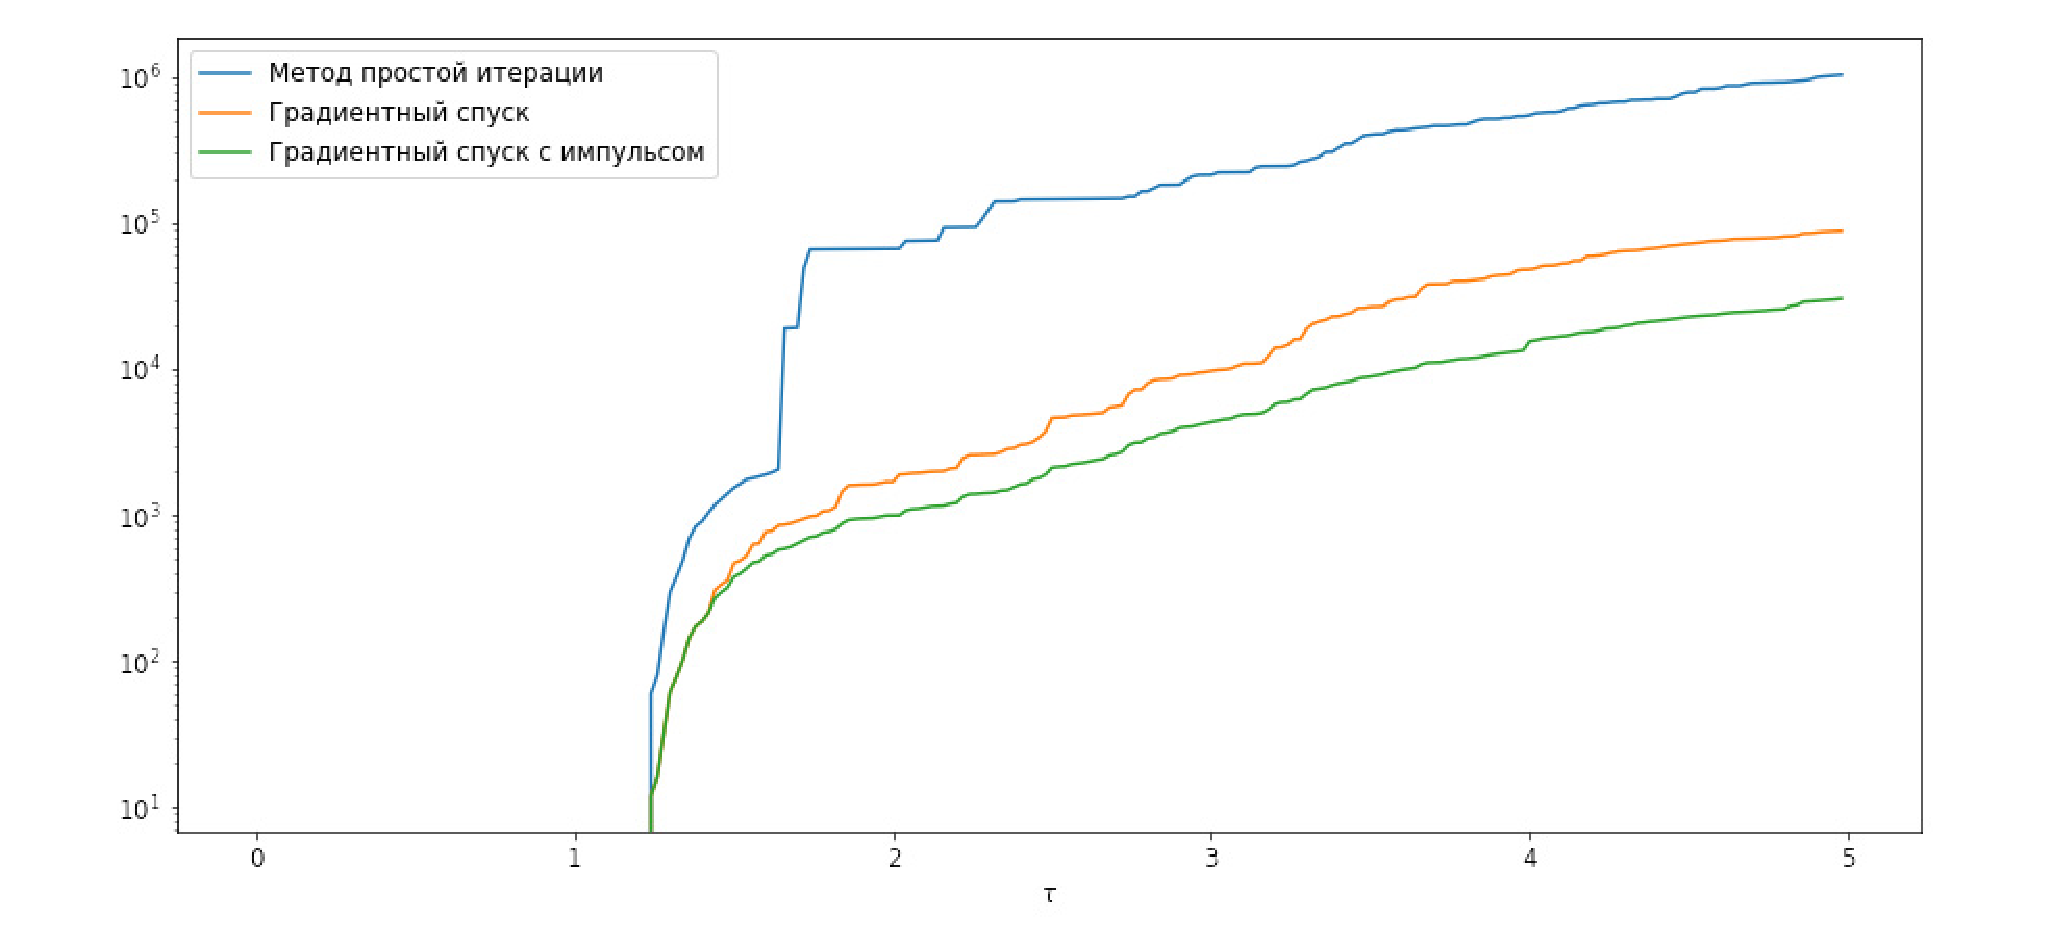
\includegraphics[width=1.0\linewidth]{comp_num_trac.eps}
\caption{Сравнение общего числа дополнительных трассировок для каждого метода.}
\label{fig:comp_num_trac}
\end{figure}

\noindentРис. \ref{fig:comp_num_trac} подтверждает ранее сделанный вывод.

Теперь продемонстрируем относительную эффективность градиентных методов по сравнению с методом простой итерации.

\begin{figure}[H] 
\centering
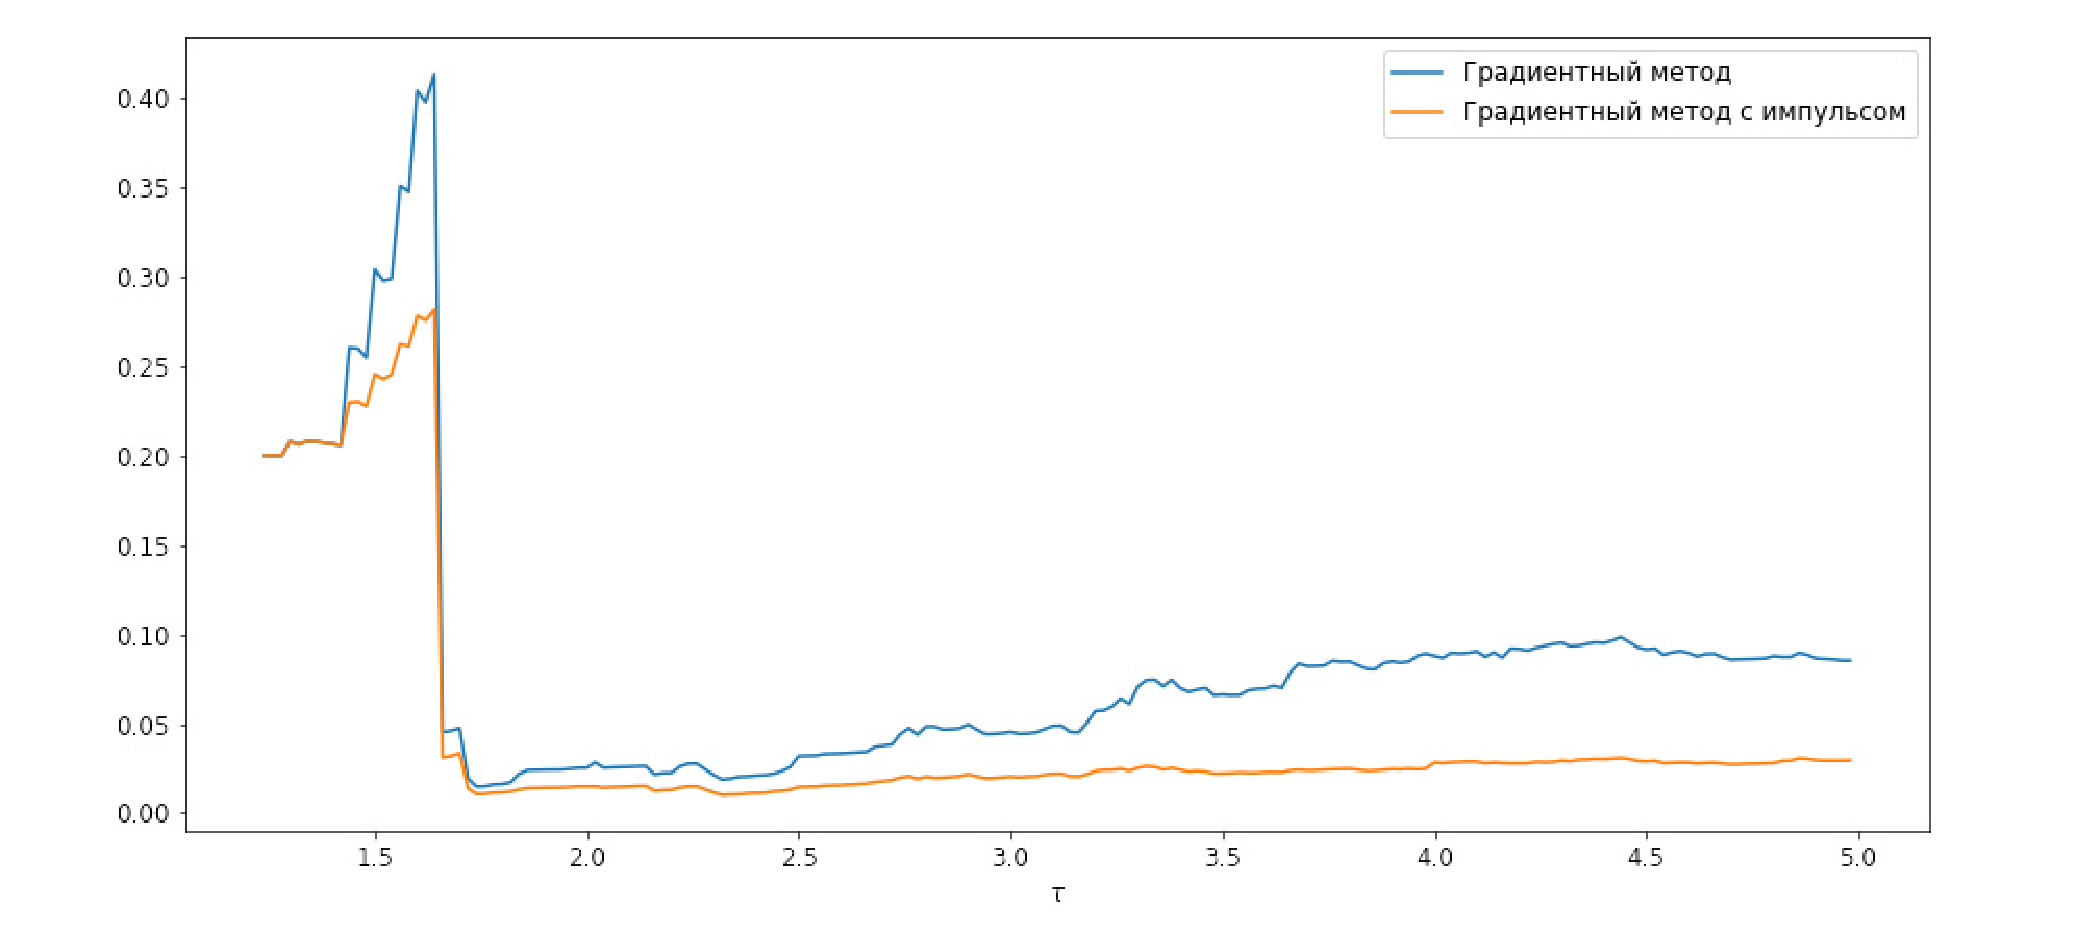
\includegraphics[width=1.0\linewidth]{comp_complexity.eps}
\caption{Эффективность градиентных методов.}
\label{fig:comp_complexity}
\end{figure}

\noindentИз рис. \ref{fig:comp_complexity} можно сделать вывод, что градиентный спуск в 14 раз эффективнее метода простой итерации, а градиентный спуск с импульсом -- в 40 раз.

Также сравним эффективность градиентного спуска с импульсом по сравнению с простым градиентным спуском.
\begin{figure}[H] 
\centering
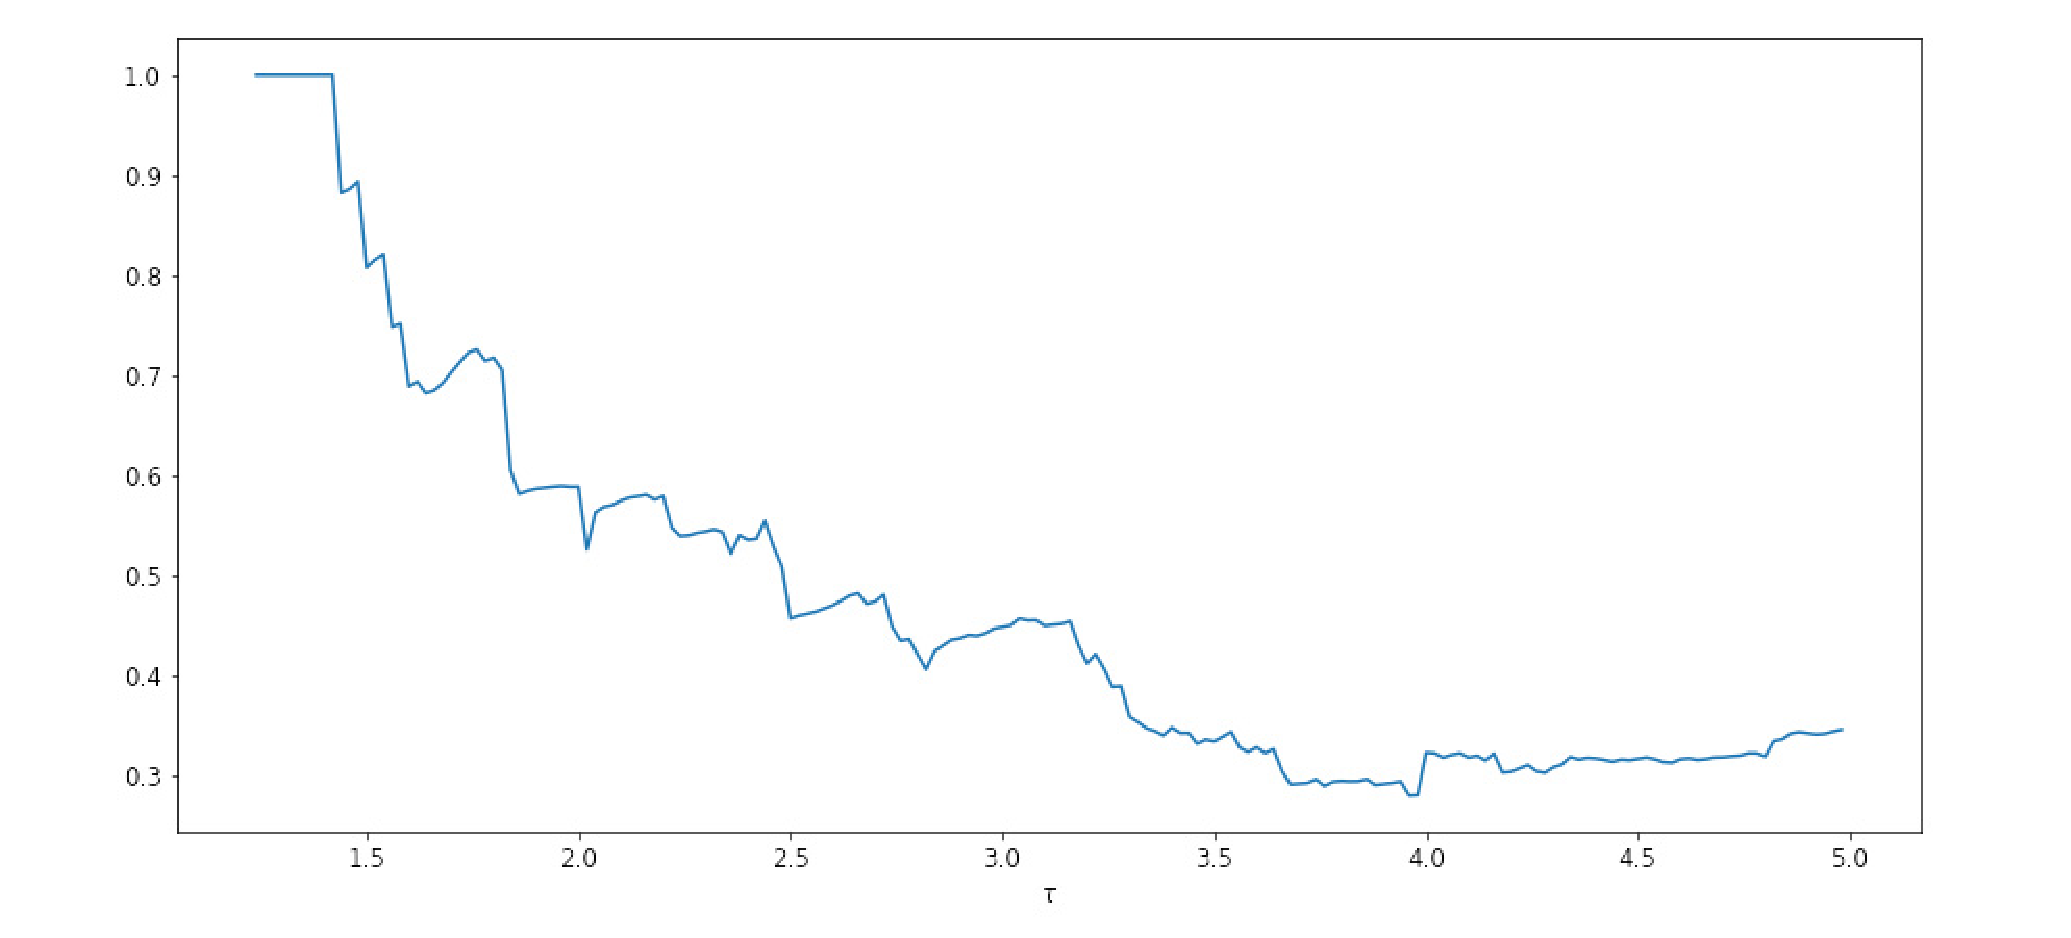
\includegraphics[width=1.0\linewidth]{comp_grad_complexity.eps}
\caption{Эффективность градиентного спуска с импульсом.}
\label{fig:comp_grad_complexity}
\end{figure}

\noindentИз рис. \ref{fig:comp_grad_complexity} можно сделать вывод, что градиентный спуск с импульсом в 2,5 раза эффективнее простого градиентный спуска.

%--------------------------------------------------------------------------------------------------------
\newpage
\anonsection{Заключение}
В ходе работы разработано два решения нелинейной краевой обратной задачи: методом прямого перебора лучей внутри лучевых трубок и градиентным методом. В качестве оптимизаторов для градиентных методов были использованы градиентный спуск и градиентный спуск с импульсом.

Далее были реализованы алгоритмы решения прямой и обратной задачи с использованием средств языка C++ и библиотеки aiwlib. Их работоспособность была проверена на тестовых данных, а также было проведено сравнение их эффективности. 

В качестве дальнейшей работы над задачей предполагается исследовать возможность применение всей информации, получаемой в ходе дополнительных трассировок, а также ускорение работы алгоритмов за счет использования параллельных вычислений.
%--------------------------------------------------------------------------------------------------------
\newpage
\bibliography{biblio/lib}
%--------------------------------------------------------------------------------------------------------
\newpage
\anonsection{Приложение}
\begin{figure}[h] 
\centering
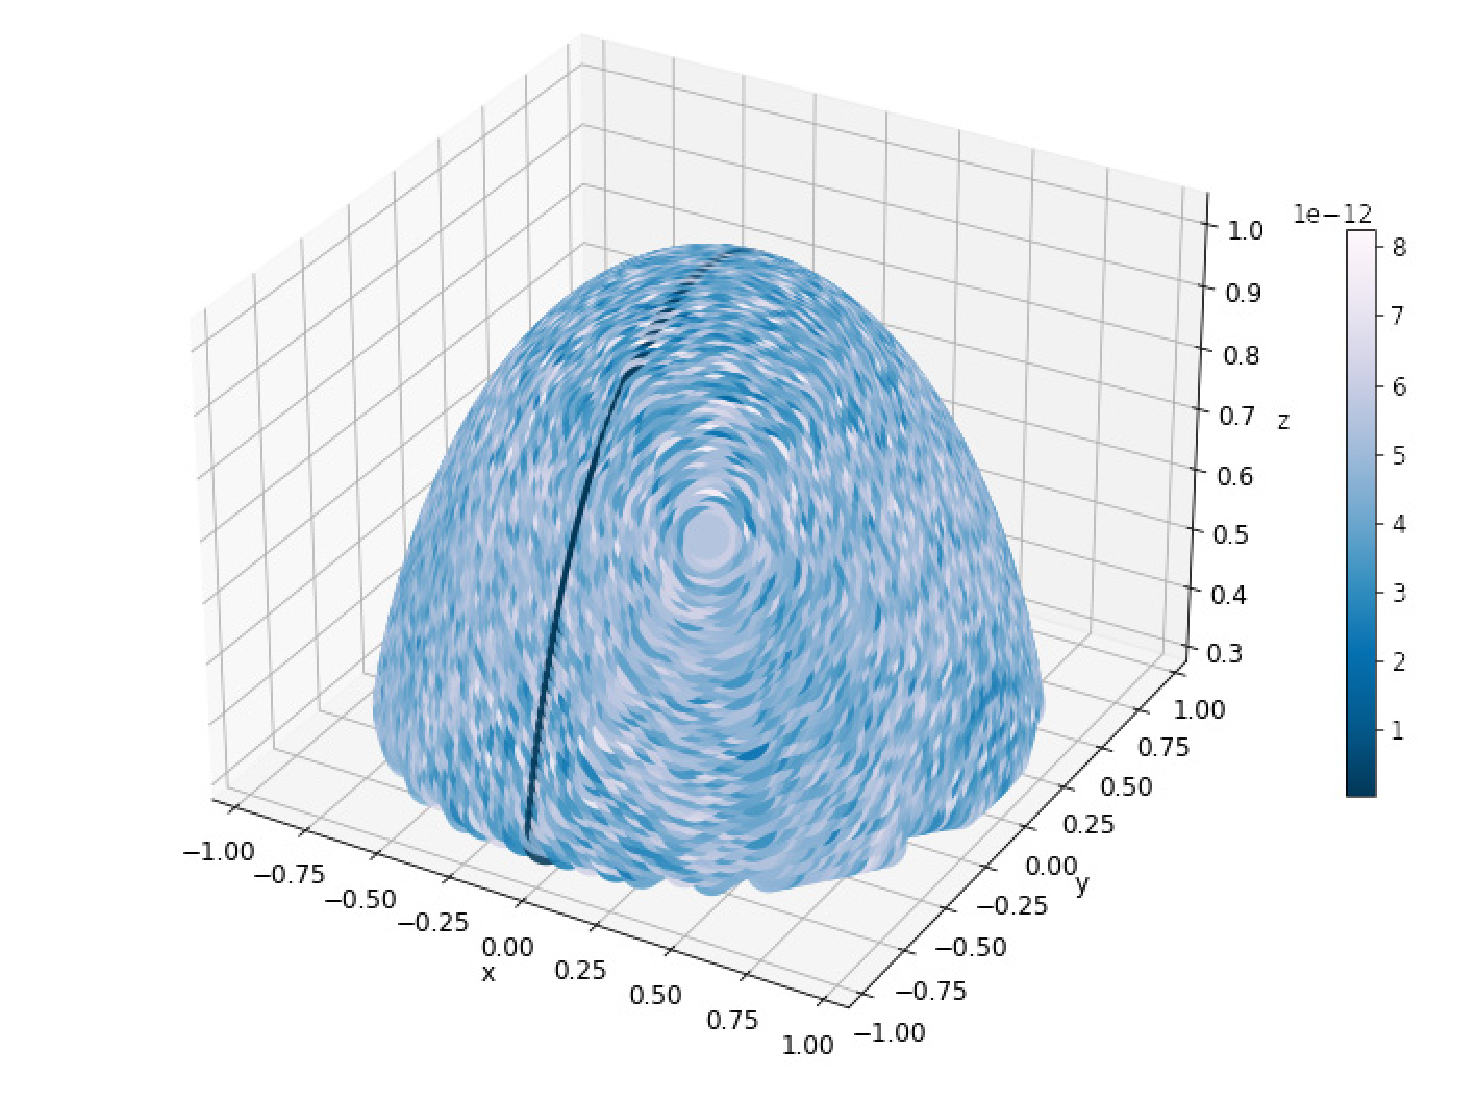
\includegraphics[width=1.0\linewidth]{grad_const.eps}
\caption{\textit{Константное поле скоростей.} Распределение максимальных норм ошибки для различных $\bfv{n}$ и норм $\dn_0$ в заданные моменты времени $\tau = 2.5$\,с.}
\label{fig:grad_const}
\end{figure}

\begin{figure}[h] 
\centering
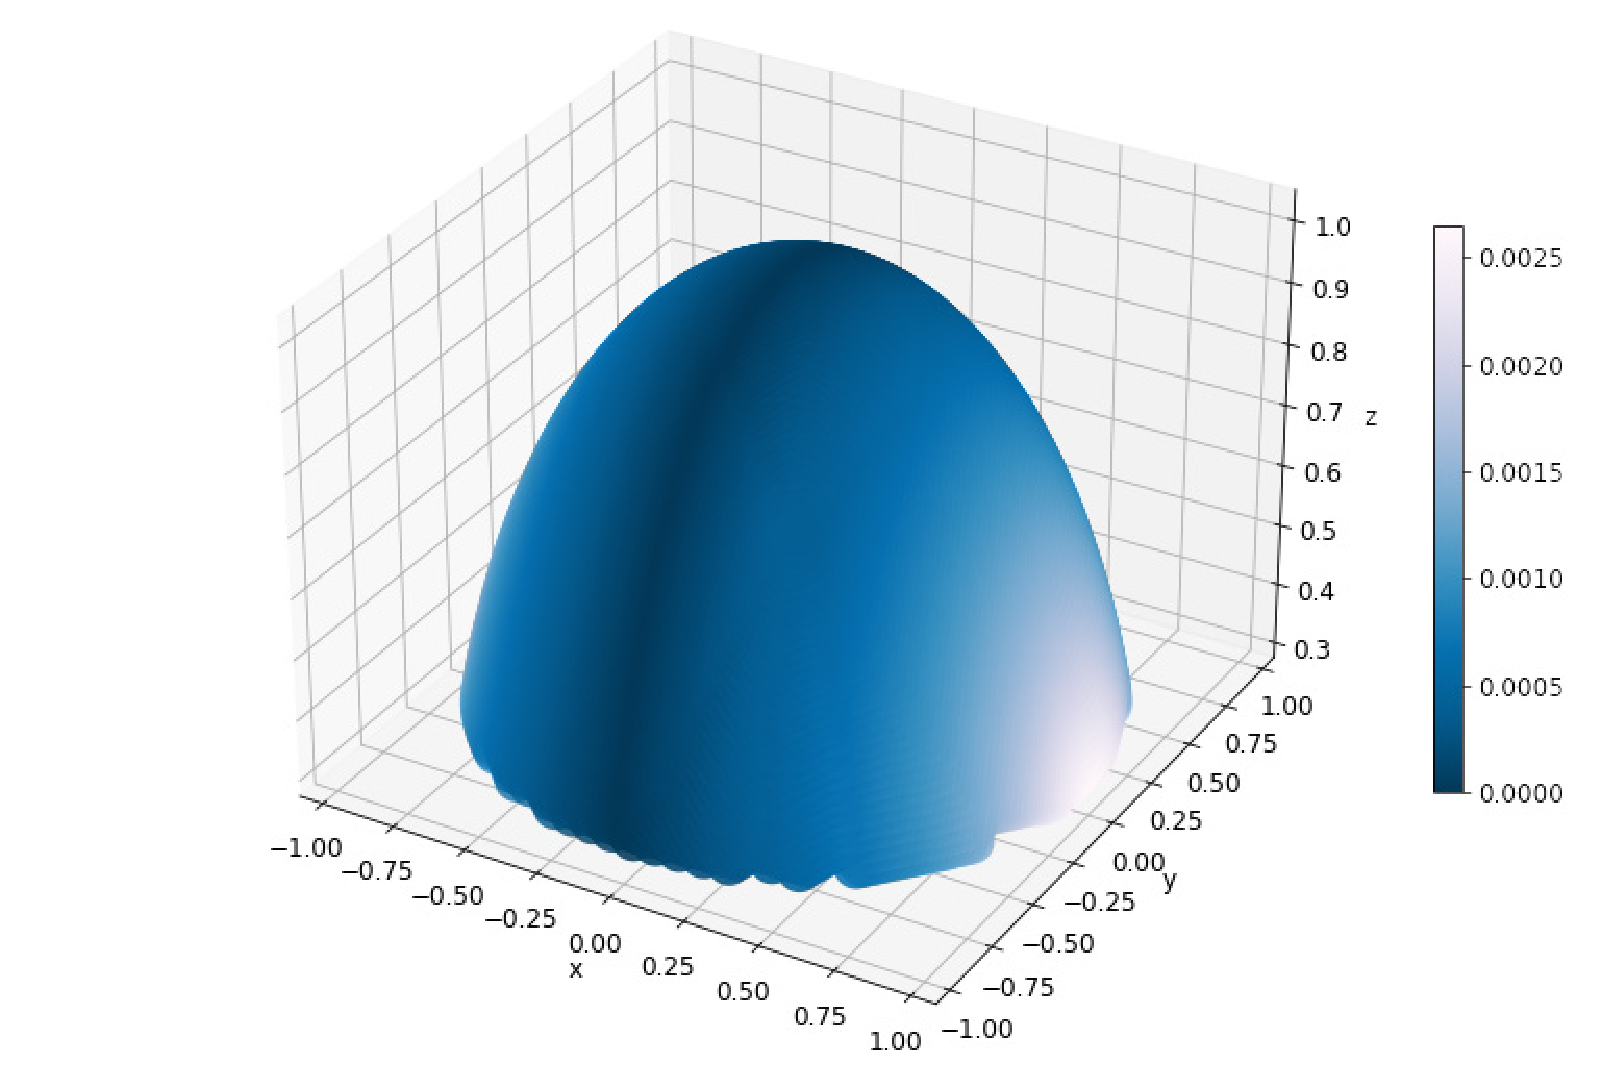
\includegraphics[width=1.0\linewidth]{grad_lin.eps}
\caption{\textit{Линейное поле скоростей.} Максимальные нормы ошибки для различных $\bfv{n}$ и норм $\dn_0$ в заданные моменты времени $\tau = 1.6$\,с.}
\label{fig:grad_lin}
\end{figure}

\begin{figure}[h] 
\centering
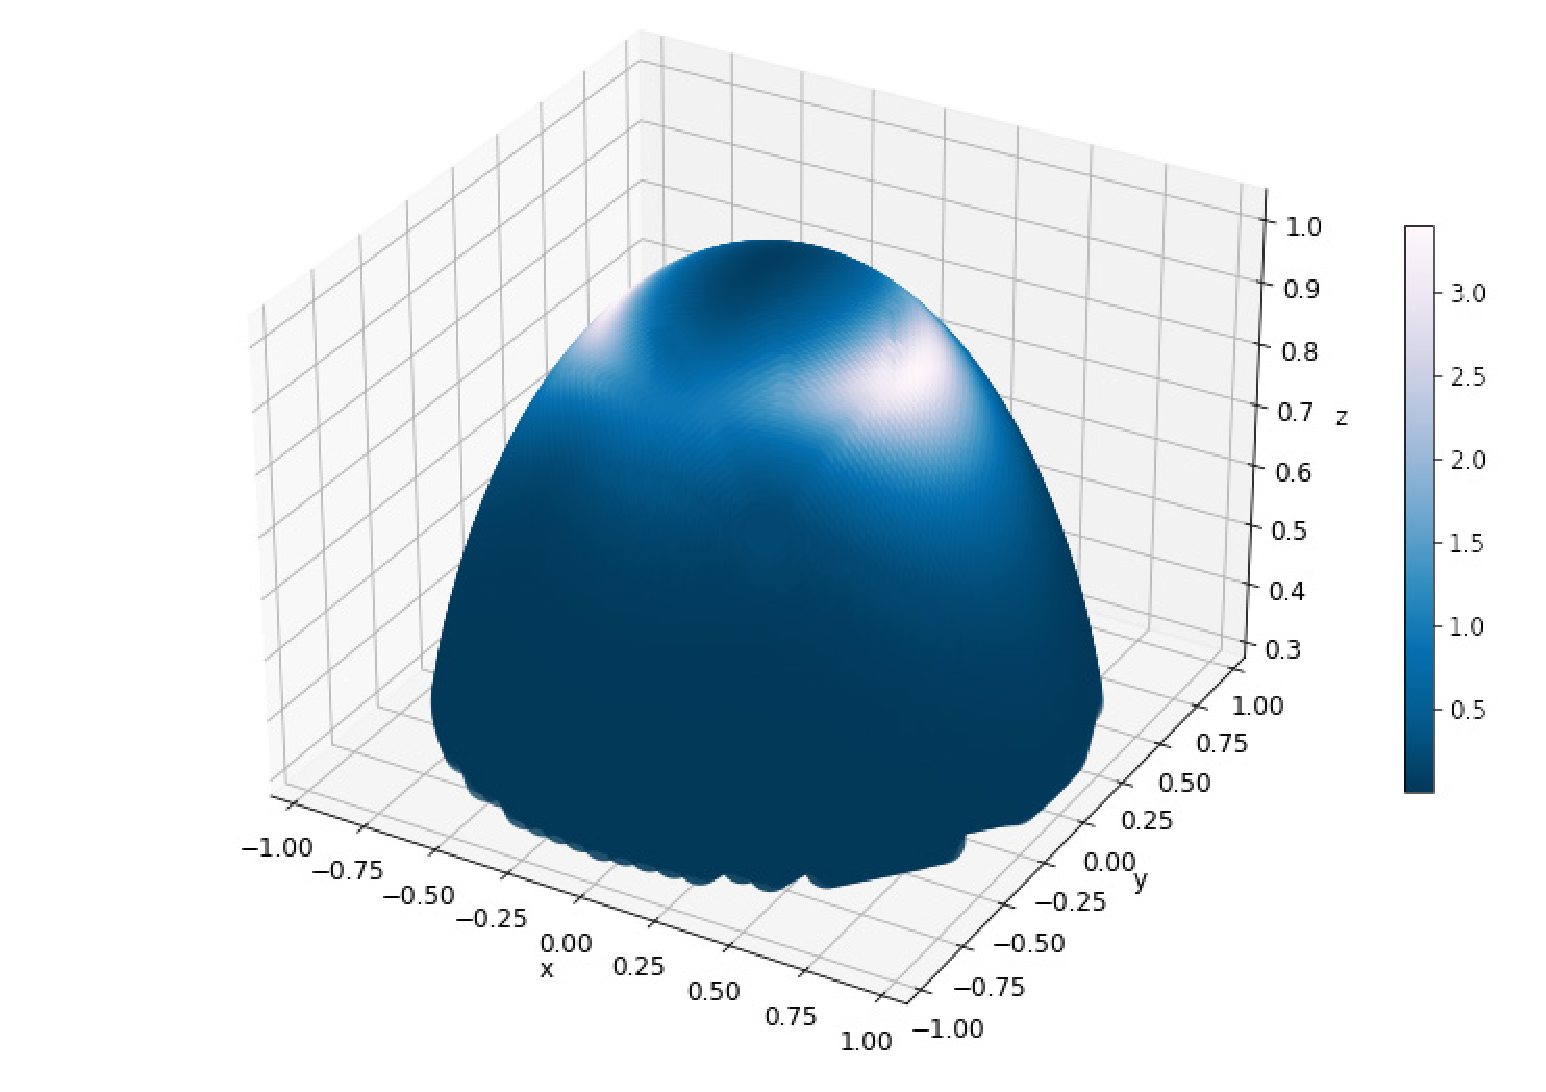
\includegraphics[width=1.0\linewidth]{grad_gauss.eps}
\caption{\textit{Модельное поле скоростей.} Максимальные нормы ошибки для различных $\bfv{n}$ и норм $\dn_0$ в заданные моменты времени $\tau = 1.6$\,с.}
\label{fig:grad_gauss}
\end{figure}

\begin{figure}[h] 
\centering
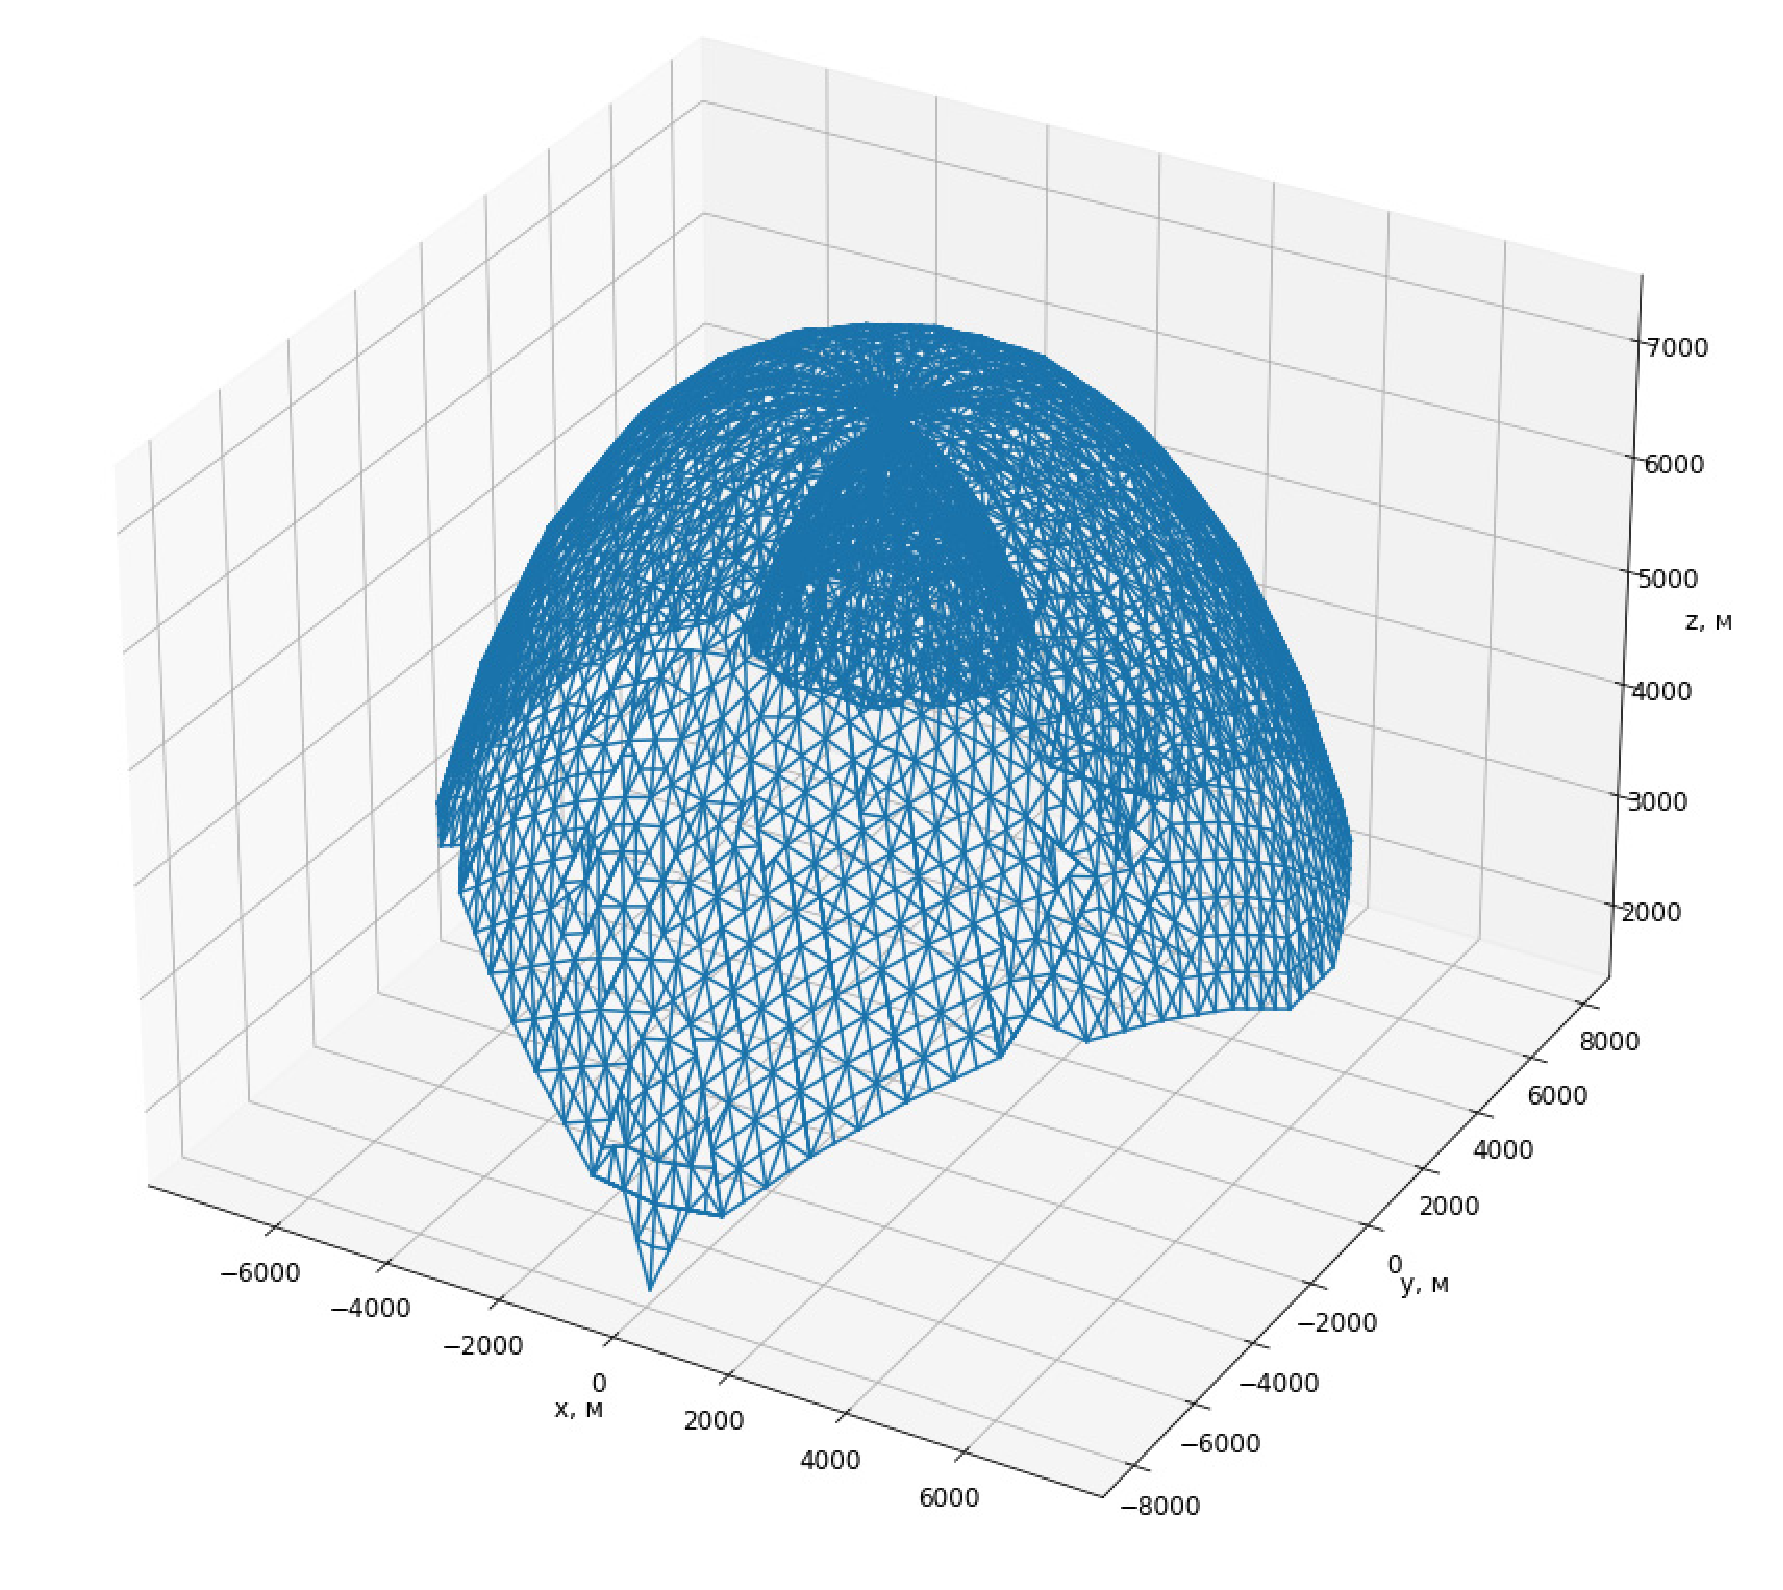
\includegraphics[width=1.0\linewidth]{direct_search.eps}
\caption{Волновой фронт при решении задачи методом прямого поиска в момент времени $\tau = 4$\,с.}
\label{fig:direct_search}
\end{figure}


\begin{figure}[h] 
\centering
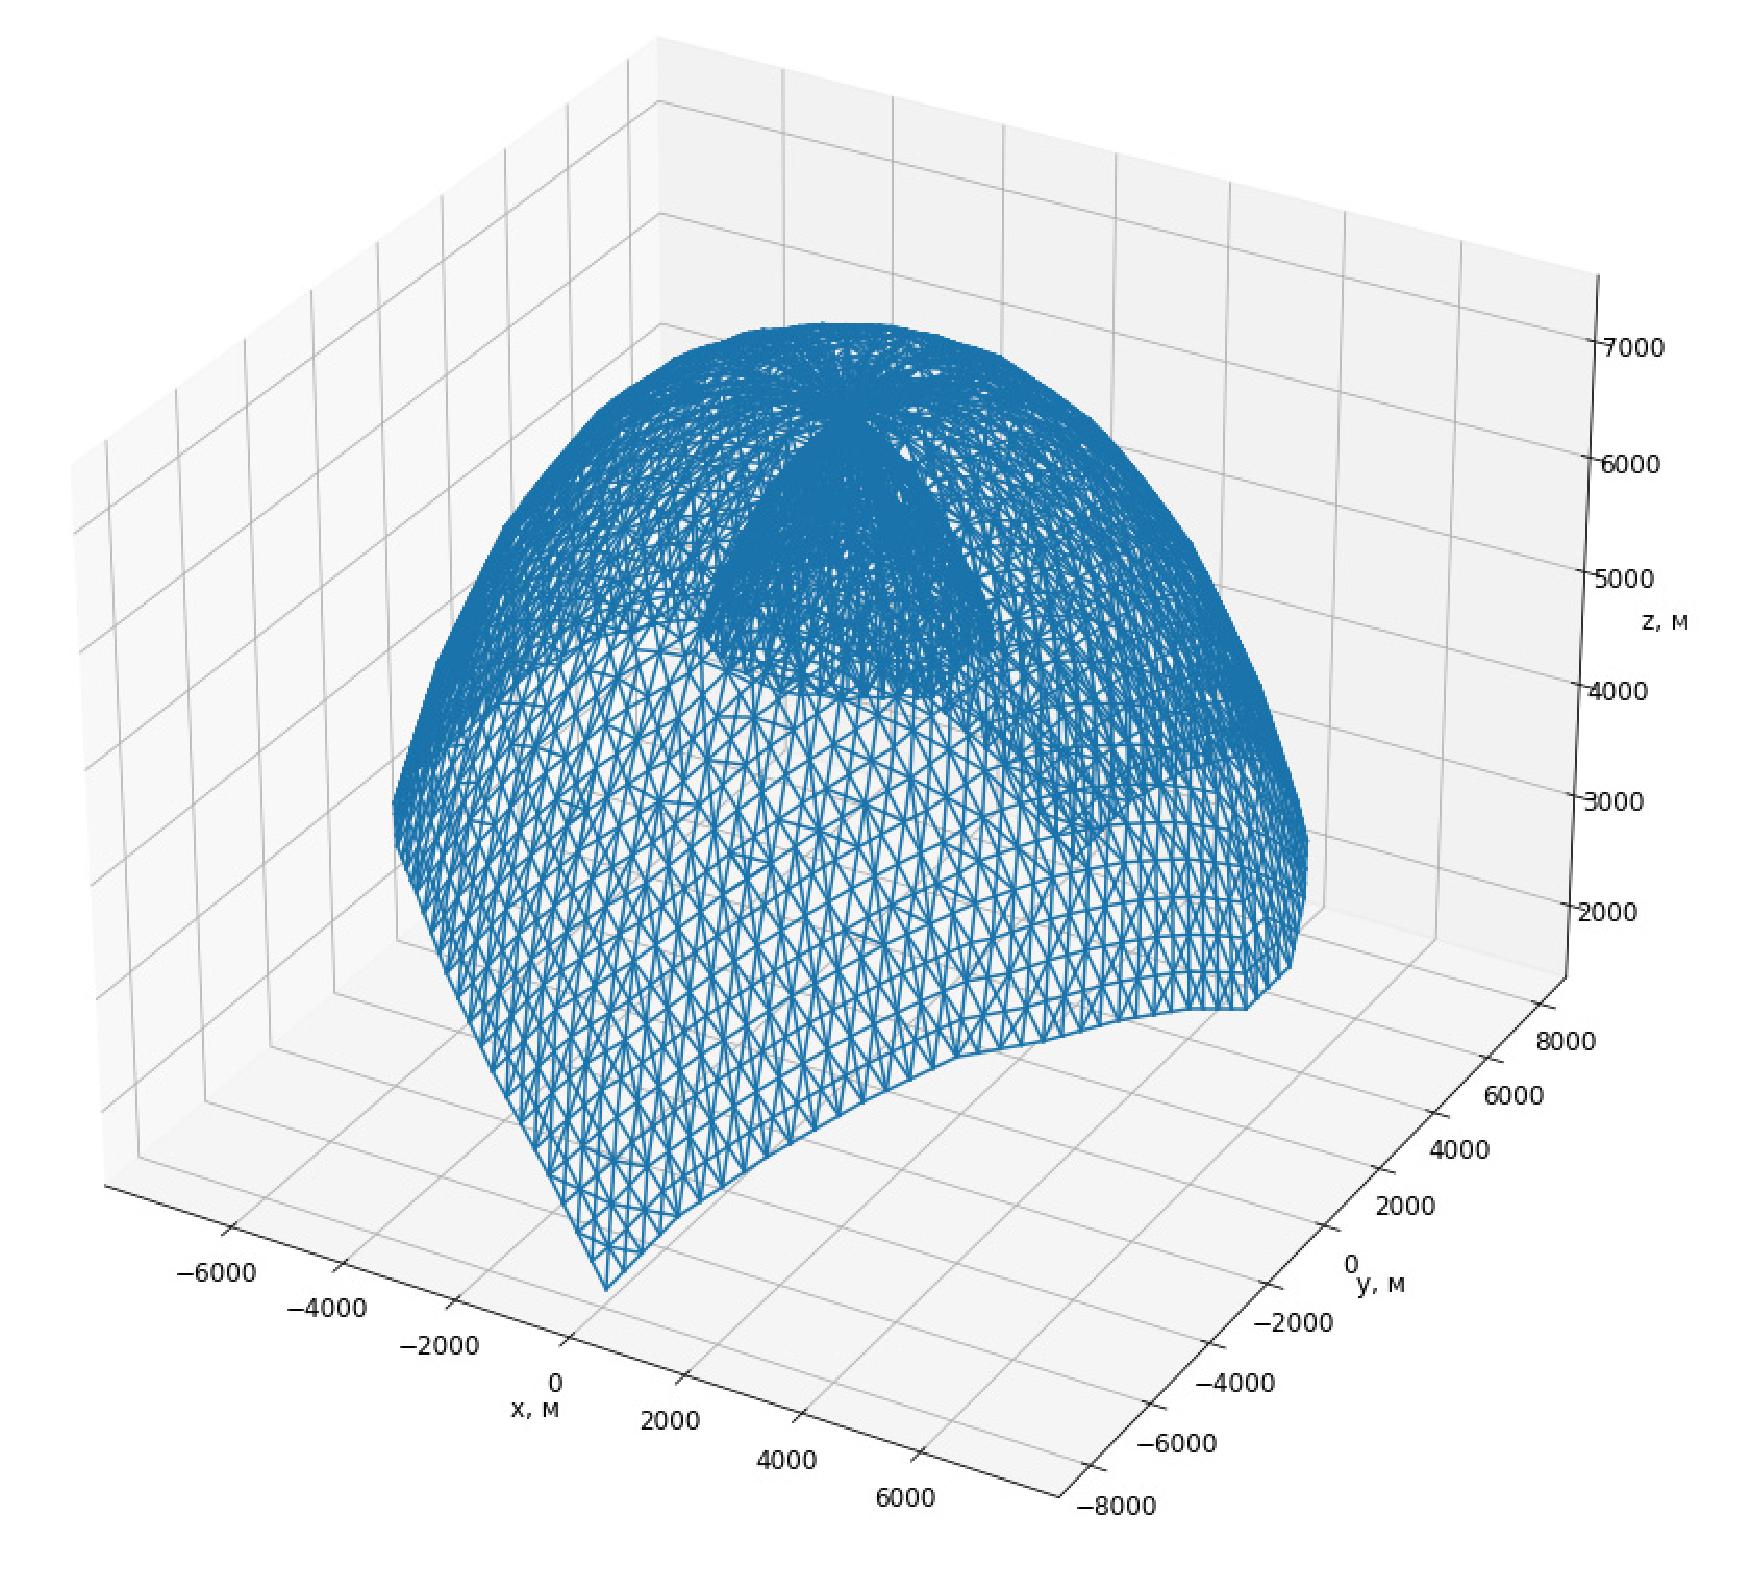
\includegraphics[width=1.0\linewidth]{grad_step.eps}
\caption{Волновой фронт при решении задачи методом градиентного спуска в момент времени $\tau = 4$\,с.}
\label{fig:grad_step}
\end{figure}

\begin{figure}[h] 
\centering
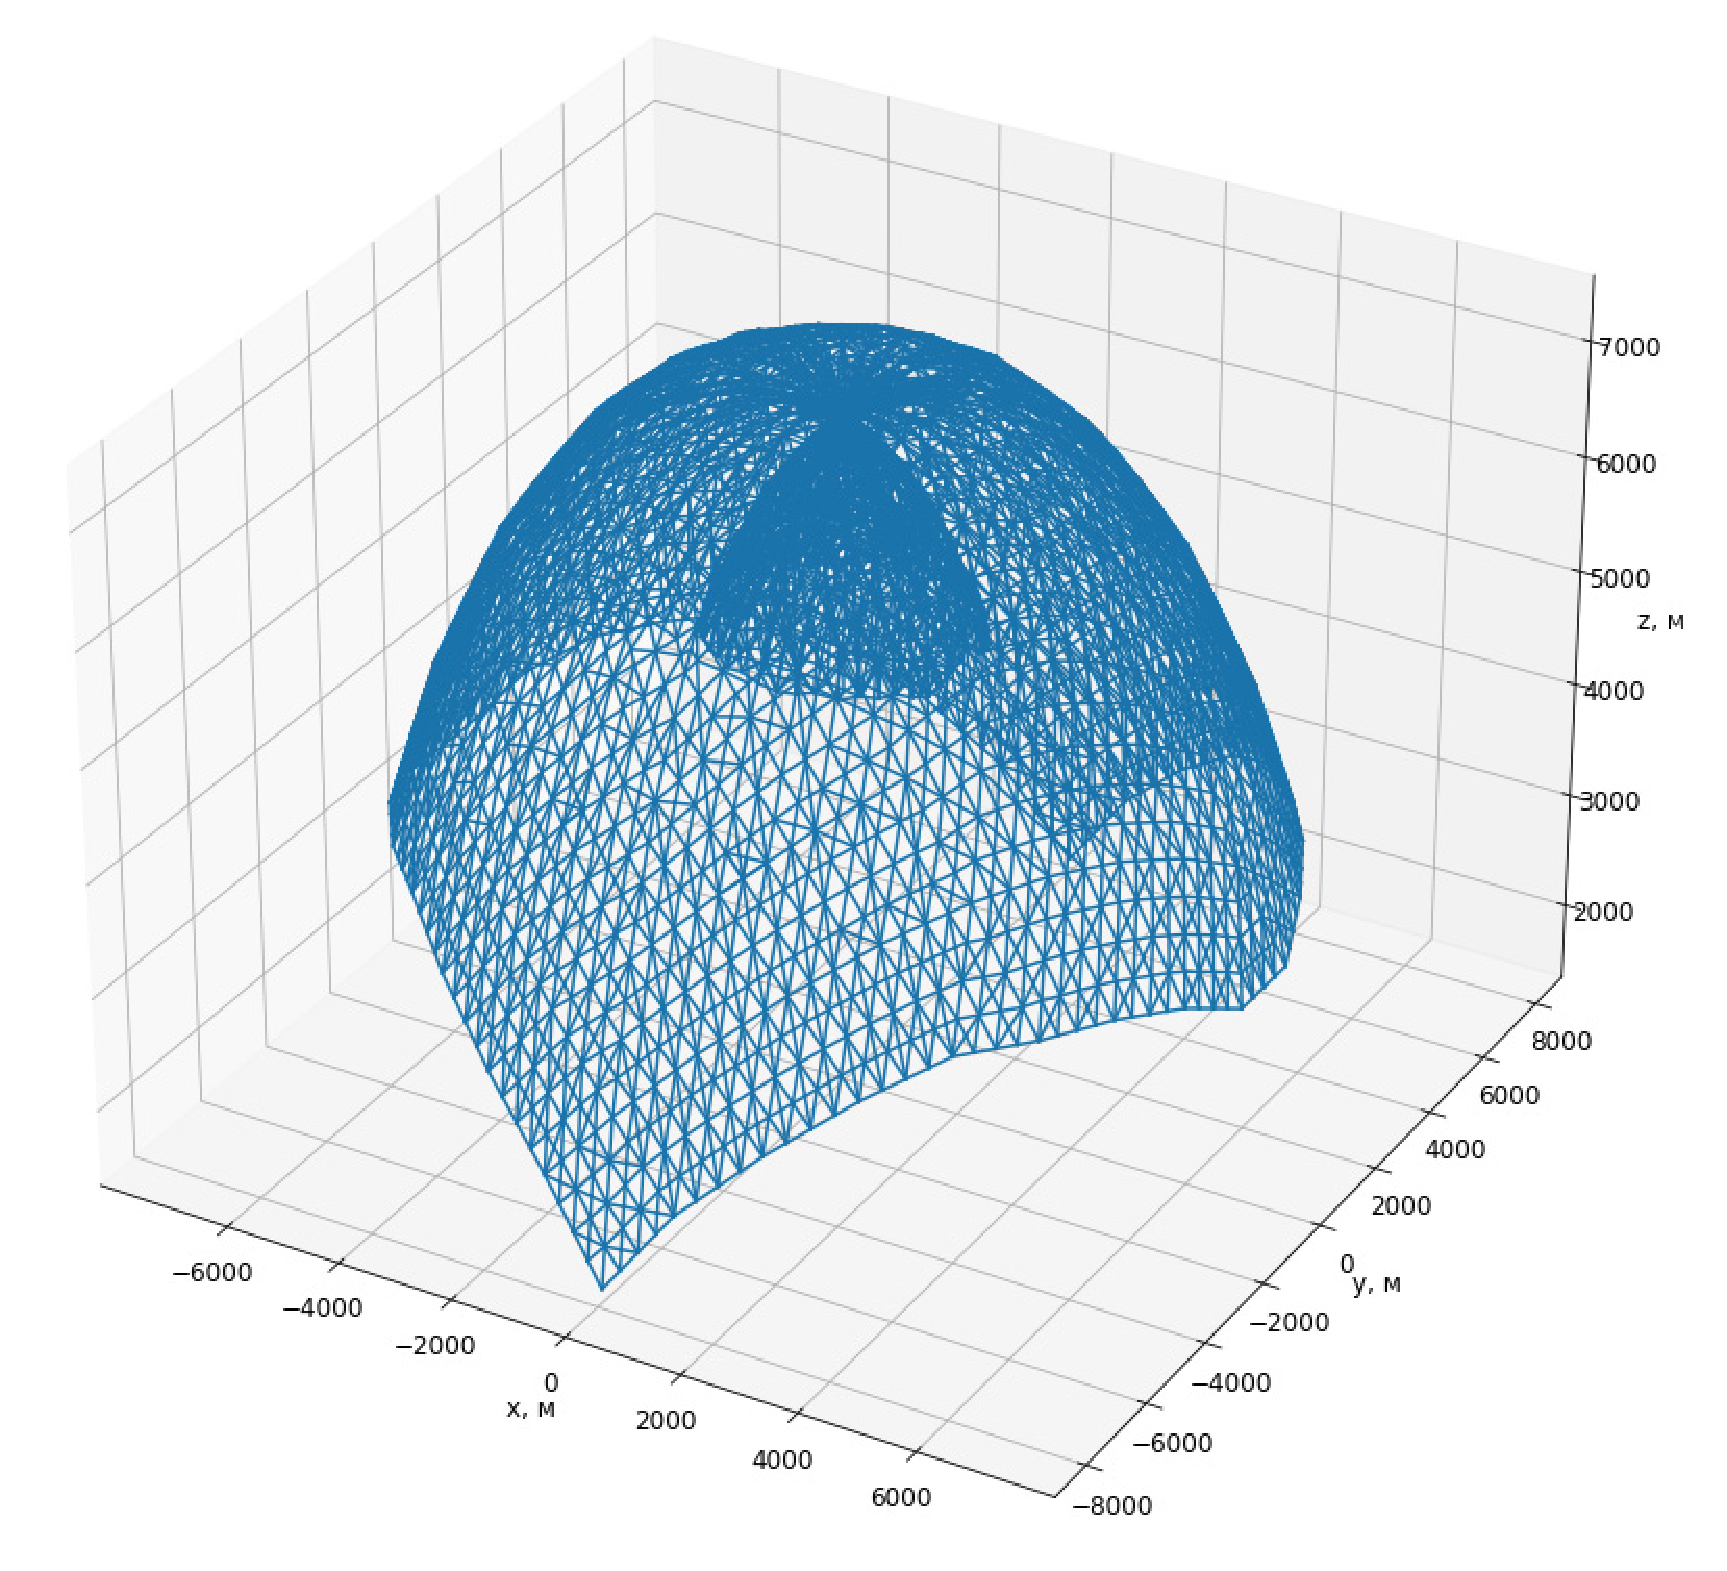
\includegraphics[width=1.0\linewidth]{grad_impulse.eps}
\caption{Волновой фронт при решении задачи методом градиентного спуска с импульсом в момент времени $\tau = 4$\,с.}
\label{fig:grad_impulse}
\end{figure}

\end{document}
